\documentclass[12pt,a4paper,oneside]{report}             % Single-side
%\documentclass[11pt,a4paper,twoside,openright]{report}  % Duplex

%\PassOptionsToPackage{chapternumber=Huordinal}{magyar.ldf}
\usepackage{t1enc}
\usepackage[utf8]{inputenc}
\usepackage{amsmath}
\usepackage{amssymb}
\usepackage{enumerate}
%\usepackage[thmmarks]{ntheorem}
\usepackage{graphics}
\usepackage{epsfig}
\usepackage{listings}
\usepackage{color}
\usepackage{fancyhdr}
\usepackage{lastpage}
\usepackage{anysize}
\usepackage{amsthm}
\usepackage[magyar]{babel}
%\usepackage{indentfirst}
%\usepackage{natbib}
\usepackage{sectsty}
\usepackage{setspace}  % Ettol a tablazatok, abrak, labjegyzetek maradnak 1-es sorkozzel!
\usepackage[hang,compatibility=false]{caption}
%\usepackage{hyperref}
\usepackage{bookmark}


\newtheorem{definition}{Def}

%--------------------------------------------------------------------------------------
% Main variables
%--------------------------------------------------------------------------------------
\newcommand{\mitauthor}{Kovács Balázs}
\newcommand{\mitadvisor}{Kertész Zsolt}
\newcommand{\mittitle}{Tekintetkövető rendszer fejlesztése képfeldolgozási alapokon}

%--------------------------------------------------------------------------------------
% Custom hyphenations
%--------------------------------------------------------------------------------------
\hyphenation{OpenCV}
\hyphenation{Linux}
\hyphenation{Ubuntu}
\hyphenation{toolkit}
\hyphenation{wxWidgets}
\hyphenation{AdaBoost}

%--------------------------------------------------------------------------------------
% Redefine original \chapter and \section commands
%--------------------------------------------------------------------------------------
\let\oldchap=\chapter
\renewcommand*{\chapter}{\secdef{\chapternostar}{\chapterstar}}
%\newcommand\chapterstar[1]{\oldchap*{#1}\markboth{~}{#1}\addcontentsline{toc}{chapter}{#1}}
\newcommand\chapterstar[1]{\phantomsection\addcontentsline{toc}{chapter}{#1}\oldchap*{#1}\markboth{~}{#1}}
%The first argument to \chapter is optional, hence the need for "[]"
%in the following definition. However, \secdef duplicates the mandatory
%argument if no optional argument was given. So we'll always have that
%argument and the default doesn't matter.
%\newcommand\chapternostar[2][]{\oldchap[#1]{#2}\markboth{\thechapter. #1}{\thechapter. #1}}
\newcommand\chapternostar[2][]{\phantomsection\oldchap[#1]{#2}\markboth{\thechapter. #1}{\thechapter. #1}}

\let\oldsect=\section
\renewcommand*{\section}{\secdef{\sectionnostar}{\sectionstar}}
%\newcommand\sectionstar[1]{\oldsect{#1}\markright{\thesection. #1}}
\newcommand\sectionstar[1]{\phantomsection\oldsect{#1}\markright{\thesection. #1}}
%\newcommand\sectionnostar[2][]{\oldsect[#1]{#2}\markright{\thesection. #1}}
\newcommand\sectionnostar[2][]{\phantomsection\oldsect[#1]{#2}\markright{\thesection. #1}}

\let\oldsubsect=\subsection
\renewcommand*{\subsection}{\secdef{\subsectionnostar}{\subsectionstar}}
\newcommand\subsectionstar[1]{\phantomsection\oldsubsect{#1}\markright{\thesection. #1}}
\newcommand\subsectionnostar[2][]{\phantomsection\oldsubsect[#1]{#2}\markright{\thesection. #1}}

\let\oldsubsubsect=\subsubsection
\renewcommand*{\subsubsection}{\secdef{\subsubsectionnostar}{\subsubsectionstar}}
\newcommand\subsubsectionstar[1]{\phantomsection\oldsubsubsect{#1}\markright{\thesection. #1}}
\newcommand\subsubsectionnostar[2][]{\phantomsection\oldsubsubsect[#1]{#2}\markright{\thesection. #1}}

%--------------------------------------------------------------------------------------
% Page layout setup
%--------------------------------------------------------------------------------------
% we need to redefine the pagestyle plain
% another possibility is to use the body of this command without \fancypagestyle
% and use \pagestyle{fancy} but in that case the special pages
% (like the ToC, the References, and the Chapter pages)remain in plane style
\fancypagestyle{plain}
{
	\fancyhead[R]{}
	\fancyhead[CO]{\bfseries\footnotesize\nouppercase{\rightmark}}
	\fancyhead[C]{\bfseries\footnotesize\nouppercase{\leftmark}}
	\fancyhead[L]{}
	\fancyfoot[L,RO]{}%\thepage}%{\thepage\pageref{LastPage}}
	\fancyfoot[C]{\thepage}
	\fancyfoot[LO,R]{}
	\renewcommand{\headrulewidth}{0.4pt}
%	\renewcommand{\footrulewidth}{0.4pt}
}

\pagestyle{plain}
\setlength{\headheight}{15pt}
%\setlength{\parindent}{0pt} % áttekinthetőbb, angol nyelvű dokumentumokban jellemző
%\setlength{\parskip}{8pt plus 3pt minus 3pt} % áttekinthetőbb, angol nyelvű dokumentumokban jellemző
\setlength{\parindent}{12pt} % magyar nyelvű dokumentumokban jellemző
\setlength{\parskip}{0pt}    % magyar nyelvű dokumentumokban jellemző

\marginsize{35mm}{25mm}{15mm}{15mm} % anysize package
\setcounter{secnumdepth}{0}
%\setcitestyle{authoryear, round, comma, aysep={;}, yysep={,}, notesep={, }}
\sectionfont{\Large\upshape\bfseries}
\subsectionfont{\large\upshape\bfseries}

\setcounter{secnumdepth}{2}
\singlespacing
\frenchspacing

%--------------------------------------------------------------------------------------
%	Setup hyperref package
%--------------------------------------------------------------------------------------
\hypersetup{
    %bookmarks=true,           % show bookmarks bar?
    bookmarksnumbered=true,   % set numbering
    unicode=true,             % non-Latin characters in Acrobat’s bookmarks
    pdftitle={\mittitle},     % title
    pdfauthor={\mitauthor},   % author
    pdfsubject={diplomaterv},   % subject of the document
    pdfcreator={\mitauthor},  % creator of the document
    pdfproducer={Kovács Balázs},   % producer of the document
    pdfkeywords={tekintetkövetés, gaze tracking, képfeldolgozás, image processing},   % list of keywords
    pdfnewwindow=true,        % links in new window
    colorlinks=true,          % false: boxed links; true: colored links
    linkcolor=black,          % color of internal links
    citecolor=black,          % color of links to bibliography
    filecolor=black,          % color of file links
    urlcolor=black            % color of external links
}
%--------------------------------------------------------------------------------------
%	Some new commands and declarations
%--------------------------------------------------------------------------------------
\renewcommand{\captionfont}{\small\itshape}
\renewcommand{\captionlabelfont}{\small\upshape\bfseries}
\newcommand{\code}[1]{{\upshape\ttfamily\scriptsize\indent #1}}
%\newcommand{\url}[1]{{\upshape\ttfamily\normalsize #1}}

% define references
\newcommand{\figref}[1]{\ref{fig:#1}.}
\renewcommand{\eqref}[1]{(\ref{eq:#1})}
\newcommand{\listref}[1]{\ref{listing:#1}.}
\newcommand{\sectref}[1]{\ref{sect:#1}.}
\newcommand{\tabref}[1]{\ref{tab:#1}.}

\DeclareMathOperator*{\argmax}{arg\,max}
%\DeclareMathOperator*[1]{\floor}{arg\,max}
\DeclareMathOperator{\sign}{sgn}
\DeclareMathOperator{\rot}{rot}
\definecolor{lightgray}{rgb}{0.95,0.95,0.95}

\author{\mitauthor, \mitauthork}
\title{\mittitle}
\includeonly{
	preliminaries,%
	statement,
	abstract,
	introduction,%
	chapter1,%
	chapter2,%
	chapter3,%
	chapter4,%
	chapter5,%
	chapter6,%
	assessment,%
	acknowledgement,%
	appendices,%
}
%--------------------------------------------------------------------------------------
%	Setup captions
%--------------------------------------------------------------------------------------
\captionsetup[figure]{
%labelsep=none,
%font={footnotesize,it},
%justification=justified,
width=.75\textwidth,
aboveskip=10pt}

\renewcommand{\captionlabelfont}{\small\bf}
\renewcommand{\captionfont}{\footnotesize\it}

%--------------------------------------------------------------------------------------
% Table of contents and the main text
%--------------------------------------------------------------------------------------
\begin{document}

\singlespacing
%--------------------------------------------------------------------------------------
%	The title page
%--------------------------------------------------------------------------------------
\begin{titlepage}
\begin{center}

\pdfbookmark[0]{Címoldal}{titlepage}

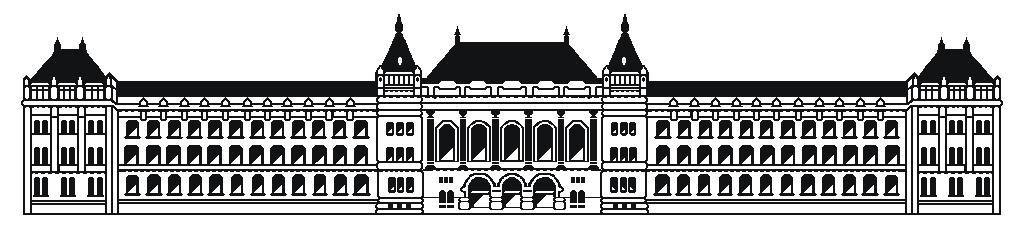
\includegraphics[width=100mm,keepaspectratio]{figures/BMElogo.png}\\
\textsc{Budapesti Műszaki és Gazdaságtudományi Egyetem}\\
\textsc{Villamosmérnöki és Informatikai Kar}\\
\textsc{Irányítástechnika és Informatika Tanszék}\\[5cm]

\vspace{0.4cm}
{\huge \bfseries \mittitle}\\[0.8cm]
\vspace{0.5cm}
\textsc{\Large Diplomaterv}\\[4cm]

\begin{tabular}{cc}
 \makebox[7cm]{\emph{Készítette}} & \makebox[7cm]{\emph{Konzulens}} \\
 \makebox[7cm]{\mitauthor} & \makebox[7cm]{\mitadvisor}
\end{tabular}

\vfill
{\large \today}
\end{center}
\end{titlepage}

%--------------------------------------------------------------------------------------
% Set up listings
%--------------------------------------------------------------------------------------
\lstset{
	basicstyle=\scriptsize\ttfamily, % print whole listing small
	keywordstyle=\color{black}\bfseries\underbar, % underlined bold black keywords
	identifierstyle=, 					% nothing happens
	commentstyle=\color{white}, % white comments
	stringstyle=\scriptsize\sffamily, 			% typewriter type for strings
	showstringspaces=false,     % no special string spaces
	aboveskip=3pt,
	belowskip=3pt,
	columns=fixed,
	backgroundcolor=\color{lightgray},
} 		
\def\lstlistingname{lista}

%\newpage\thispagestyle{empty} % an empty page

\pagenumbering{Roman}
\tableofcontents\vfill\markboth{Tartalomjegyzék}{~}

%--------------------------------------------------------------------------------------
% Nyilatkozat
%--------------------------------------------------------------------------------------
\begin{center}
\phantomsection
\addcontentsline{toc}{chapter}{Hallgatói nyilatkozat}
\large
\textbf{HALLGATÓI NYILATKOZAT}\\
\end{center}

Alulírott \emph{\mitauthor}, szigorló hallgató kijelentem, hogy ezt a diplomatervet meg nem engedett segítség nélkül, saját magam készítettem, csak a megadott forrásokat (szakirodalom, eszközök stb.) használtam fel. Minden olyan részt, melyet szó szerint, vagy azonos értelemben, de átfogalmazva más forrásból átvettem, egyértelműen, a forrás megadásával megjelöltem.

Hozzájárulok, hogy a jelen munkám alapadatait (szerző(k), cím, angol és magyar nyelvű tartalmi kivonat, készítés éve, konzulens(ek) neve) a BME VIK nyilvánosan hozzáférhető elektronikus formában, a munka teljes szövegét pedig az egyetem belső hálózatán keresztül (vagy autentikált felhasználók számára) közzétegye. Kijelentem, hogy a benyújtott munka és annak elektronikus verziója megegyezik. Dékáni engedéllyel titkosított diplomatervek esetén a dolgozat szövege csak 3 év eltelte után válik hozzáférhetővé.

\begin{flushleft}
\vspace*{1cm}
Budapest, \today
\end{flushleft}

\begin{flushright}
 \vspace*{1cm}
 \begin{tabular}{c}
 \makebox[7cm]{\rule{6cm}{.4pt}} \\
 \makebox[7cm]{\emph{\mitauthor}} \\
 \makebox[7cm]{hallgató} \\
 \end{tabular}
\end{flushright}
%\thispagestyle{empty}

\vfill
%\clearpage
%\thispagestyle{empty} % an empty page
%----------------------------------------------------------------------------
% Abstract in hungarian
%----------------------------------------------------------------------------
\chapter*{Kivonat}

Jelen dokumentum egy a Budapesti Műszaki és Gazdaságtudományi Egyetem Irányítástechnika és Informatika Tanszékén készített diplomaterv \emph{,,Tekintetkövető rendszer fejlesztése képfeldolgozási alapokon''} témában. 

További szöveg.

\newpage

%----------------------------------------------------------------------------
% Abstract in english
%----------------------------------------------------------------------------
\chapter*{Abstract}

The current paper is a thesis from Department of Control Engineering and Information Technology at Budapest University of Technology and Economics in the topic of \emph{,,Development of a Gaze Tracking System Based on Image Processing''}. 

More abstract.

\vfill
%\clearpage~

\setcounter{page}{1}
\pagenumbering{arabic}
%----------------------------------------------------------------------------
\chapter*{Bevezető}
%----------------------------------------------------------------------------

\begin{verse}
\begin{flushright}
\emph{Hová merűlt el szép szemed világa? \\
Mi az, mit kétes távolban keres?} \\
\dots
\end{flushright}
\end{verse}

Tekintetkövető rendszer fejlesztése összetett feladat. A probléma mind magas, mind alacsony absztrakciós szintről megközelítve megfelelő szakmai felkészültséget követel meg: a rendszer megtervezéséhez, összeállításához és implementációjához olyan önálló mérnöki munka szükséges, ami a ideálissá tette számomra a feladatot diplomatervem témájaként.

\bigskip

A körülöttünk lévő világ megismerésében nyilvánvalóan alapvető szerepet tölt be a látás, ezen belül is a figyelmünk célzott irányítása. A vizuális feldolgozás meglétét és működését a legtöbbször olyannyira készpénznek vehetjük, hogy hajlamosak lehetünk elsiklani a tény fölött, hogy a megértés egyik első lépcsőjeként jelen lévő tekintet követése és analízise milyen mély jelentést hordozhat, legyen szó akár pszichológiai, akár fiziológiai vonatkozásokról.

A tekintet információgazdagságának köszönhetően reményeim szerint a rendszer -- valamint a fejlesztése során megszerzett tapasztalat -- remélhetőleg sok hasznos és érdekes kutatási vagy ipari felhasználásban bizonyulhat alkalmazhatónak.

\bigskip

Diplomatervem \sectref{felhasznalas} fejezetében a tekintetkövető rendszer lehetséges felhasználási területeiről nyújtok rövid áttekintést, a \sectref{tekintetkovetes} fejezetben pedig magát a tekintetkövetést veszem górcső alá a vonatkozó szakirodalomban fellelhető módszerek és a követendő szemmozgások összefoglalásával. Dolgozatom \sectref{elmeleti_alapok} fejezetében a tekintetkövetéshez felhasznált tudományos módszerek elméleti alapjait tárgyalom.

Gyakorlatiasabb vizekre evezve: a \sectref{technologia} fejezet technológiai áttekintésként szolgál, azaz bemutatom benne a fejlesztés során felhasznált szoftver- és hardverkomponenseket. Az \sectref{megvalositas_1} és \sectref{megvalositas_2} fejezetek pedig már kifejezetten a rendszer implementációjáról szólnak. A szétválasztást az indokolta, hogy amíg az \sectref{megvalositas_1} fejezetben magasabb szinten, a felesleges részletek mellőzésével mutatom be a legfontosabb feldolgozási algoritmusokat és igazolom a rendszer használhatóságát, addig a \sectref{megvalositas_2} fejezet első fele kimondottan az alkalmazás architektúrájával és az implementáció részleteivel foglalkozik.

Végezetül a \sectref{megvalositas_2} fejezet második felében dokumentálom az elkészült alkalmazás felhasználói felületét és használati eseteit, valamint összefoglalom és értékelem a munka során gyűjtött tapasztalataimat.
%----------------------------------------------------------------------------
\chapter{Felhasználási lehetőségek}\label{sect:felhasznalas}
%----------------------------------------------------------------------------

A tekintet megfelelő minőségű és robusztus követésének számos gyakorlati felhasználása lehetséges. Elég csak a kutatási területek közül a \emph{perceptuális} (észlelési), vagy \emph{kognitív} (megértési) területekre gondolni, ahol például az olvasás, vagy az alvás folyamatának vizsgálatánál bizonyulhat hasznosnak.

Nem feltétlenül kell azonban a tekintetkövetést laboratóriumok falai közé szorítani: a rendszer számos gyakorlati életből vett felhasználási területen bizonyulhat hasznosnak, például a webergonómia vagy a vezetésbiztonság területein.

\bigskip

Az előző bekezdésekben felvázolt felosztás alapján a fejezet \sectref{tudomanyos} szakaszában a kutatási, míg az \sectref{gyakorlati} szakaszban a gyakorlati felhasználási lehetőségekről nyújtok egy vállaltan nem teljes körű, sokkal inkább az érdeklődés felkeltését célzó összefoglalást.

%,,,,,,,,,,,,,,,,,,,,,,,,,,,,,,,,,,,,,,,,,,,,,,,,,,,,,,,,,,,,,,,,,,,,,,,,,,,,
\section{Kutatási felhasználás}\label{sect:tudomanyos}
%,,,,,,,,,,,,,,,,,,,,,,,,,,,,,,,,,,,,,,,,,,,,,,,,,,,,,,,,,,,,,,,,,,,,,,,,,,,,

%............................................................................
\subsection{Kognitív pszichológia}\label{sect:kognitiv}
%............................................................................

A \textbf{kognitív} (megértési) pszichológia az egyik olyan kutatási terület, amelyben a tekintetkövetés igencsak hasznos eszköz lehet, hiszen a tudományág azt vizsgálja, hogy az ember hogyan látja a világot maga körül, és milyen módon képezi le azt.

\bigskip

Csak egy a lehetséges számtalan megértési probléma közül az \textbf{olvasási folyamat} működésének analízise. Az írott szöveg megértése összetett feladat, ennek a képességnek a hiánya egy tanulási részképességzavar, a \emph{diszlexia} meglétét jelentheti. A diszlexiás állapot felismerésében, a diagnózis megerősítésében, vagy akár az okok felkutatásában lehet hasznos eszköz a tekintetkövető rendszer.

\begin{figure}[!ht]
\centering
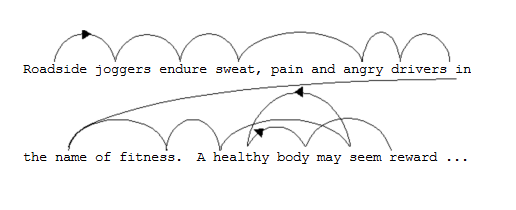
\includegraphics[width=100mm, keepaspectratio]{figures/read_saccade.png}
\caption{Szakkádok olvasás közben.\\Forrás: \url{http://bit.ly/C1ia}}
\label{fig:read_saccade}
\end{figure}

Lehetővé válhat a tekintet szakkadikus (egyszerűsítve: a tekintet trajektóriája, részletesen lásd \sectref{szakkadok} szakasz) mozgásának kellően gyors és pontos rögzítése, amely segítségével következtethetünk a megértési folyamat működésére, vagy éppen a működés hibáira. 

\bigskip

Alvásvizsgálat terén leginkább -- nevéből adódóan -- a REM (Rapid Eye Movement) fázis kötődik a szemmozgás követéséhez, ebben az alkalmazásban azonban értelemszerűen optikai elvű követés nem jöhet szóba.

%............................................................................
\subsection{Érzelemdetektálás}\label{sect:erzelem}
%............................................................................

A pupillaátmérő nem csak a fénymennyiség-változás hatására módosulhat. Érzelmi, izgalmi állapotok is előidézőik a változást, mint például félelem, idegesség vagy öröm \cite{altpszicho}. Ez a jelenség szintén potenciális felhasználási lehetőségeket rejt magában. Mivel a pupillareflex akaratlagosan nem koordinálható, állandó fénymennyiség mellett a pupillaméret változásának figyelésével detektálhatóvá válhatnak a fent említett érzelmi állapotok. Ehhez a változás mértékének és sebességének pontos mérése szükséges, ami azonban kellően nagy sebességű kamerával és elfogadható számítási teljesítményt nyújtó hardverrel kielégítő minőségben megtehető lehet. Az alkalmazás ráadásul nem feltétlenül igényli a szem közvetlen közelről (például fejre erősített kamerával) történő felvételét. Megfelelően nagy felbontású forrás esetén az arc-, majd szemrégió automatikus szegmentálása után a felismert zónát felhasználva, akár távolról is történhet a pupillareflex vizsgálata.

%............................................................................
\subsection{Orvosi felhasználás}\label{sect:orvosi_felh}
%............................................................................

Egyes betegségek is okozhatják a pupilla rendellenes méretét vagy viselkedését. Például a ,,miosis'', azaz a szem összehúzódása nemcsak a fent említett okokra vezethető vissza. Rendellenes összehúzódás alakulhat ki bizonyos patológiai állapotok, gyógyszerek, vagy mérgek hatására, sõt a mikrohullámú sugárzásnak kitett szervezet is produkálja ezt a tünetet. A ,,mydraisis'' (a pupilla tágulása) során ugyancsak nem megszokott viselkedés alakulhat ki bizonyos gyógyszerek vagy kábítószerek használatakor, de akár komoly fizikai trauma hatására is a normálisnál jelentősebb mértékű vagy időtartamú lehet a pupilla tágulata. A két szem eltérő méretű pupillája (az ,,anisocoria'') olyan betegségek meglétét jelezheti, mint a Horner-, vagy az Adie-szindróma \cite{altpszicho}. Orvosi szempontból is van tehát mit vizsgálni: a pupilla követésével egyes betegségek, állapotok felismerése, vagy alakulásuk megfigyelése laikus és orvos számára is automatizálható, megkönnyíthető lehet.

\bigskip

Továbbra is orvosi területen maradva a szemmozgás követése és regisztrálása \emph{ontoneurológiai} vizsgálatokban is szerepet kaphat. Az ilyen vizsgálat célja az egyensúlyszerv működésének megfigyelése és értékelése. Az összetett vizsgálat egyes fázisaiban a szemmozgások követése fontos információt hordoz az alany állapotáról, ugyanis a szemmozgató és az egyensúlyi információkat szállító idegpályák szoros kapcsolatban állnak egymással.

%,,,,,,,,,,,,,,,,,,,,,,,,,,,,,,,,,,,,,,,,,,,,,,,,,,,,,,,,,,,,,,,,,,,,,,,,,,,,
\section{Gyakorlati felhasználás}\label{sect:gyakorlati}
%,,,,,,,,,,,,,,,,,,,,,,,,,,,,,,,,,,,,,,,,,,,,,,,,,,,,,,,,,,,,,,,,,,,,,,,,,,,,

%............................................................................
\subsection{Webergonómia}\label{sect:webergonomia}
%............................................................................

Az ergonómia tudománya az ember és technika kapcsolatával, ezen belül is leginkább az említett kapcsolat zökkenőmentesítésével foglalkozik. 

Az ergonómia interdiszciplináris tudomány: egy ága a kapcsolat fizikai valójával foglalkozik (pl. kényelem, akadálymentes használat), egy másik terület inkább a pszichológiával rokonítható módon a fizikailag nem létező (azaz virtuális) felhasználói felületek analízisét kutatja. Ugyancsak a grafikus felületek -- azon belül kifejezetten a weboldalak -- elemzésével kapcsolatos a manapság igencsak felkapott \emph{webergonómia} területe.

\begin{figure}[!ht]
\centering
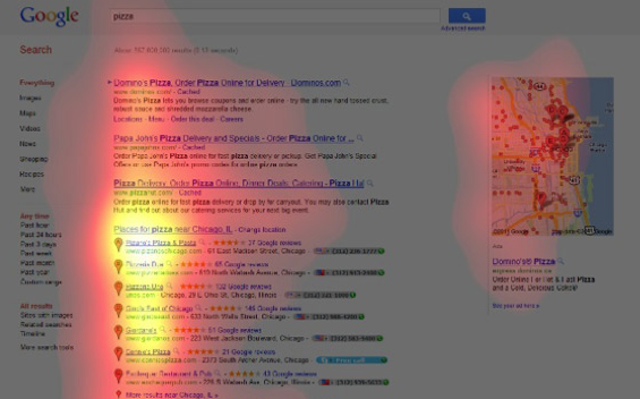
\includegraphics[width=100mm, keepaspectratio]{figures/google_heatmap.png}
\caption{A Google találati oldalának hőtérképes elemzése.\\Forrás: \url{http://on.mash.to/tHo2ap}}
\label{fig:google_heatmap}
\end{figure}

A megfelelő webes tervezés a \emph{felhasználói élmény} (user experience -- UX) szempontjából döntő fontosságú. Az elhelyezett tartalmak (legyen szó egy egyszerű honlapról, vagy egy összetett webalkalmazásról) közti navigációt úgy kell mind grafikailag, mind strukturálisan megtervezni, hogy a felhasználó intuitívan tudja használni a felületet.

Kellően pontos tekintetkövetéssel vizsgálható lehet, hogy a tervezés során mennyire sikerült a felhasználók igényeinek megfelelő felületet alkotni: könnyen eligazodnak-e rajta, esetleg idejük nagy részét a hibás tervezési döntések következtében kaotikus bolyongással töltik.

A felhasználói aktivitás rögzítésének felhasználására jó példa a \figref{google_heatmap} ábrán látható hőtérképes megjelenítés, amely a Google találati oldalának elemzésével támpontot nyújthat a keresőoptimalizálással foglalkozó szakemberek számára.

%............................................................................
\subsection{Vezetésbiztonság}\label{sect:orvosi_felhasznalas}
%............................................................................

Bár folynak már kutatások és tesztek vezető nélküli, automatizált járművek közúti használatára\footnote{például \emph{Google Driverless Car}, lásd \url{http://bit.ly/PehN2r}}, a humán faktor valószínűleg még nagyon sokáig nem lesz teljesen megkerülhető, ha autóvezetésről van szó.

Vezetésbiztonsági alkalmazásban is elképzelhető lehet a tekintetkövetés alkalmazása. A vezető fókuszának vizsgálatán túl, a követés során mintegy járulékos információként mérhetjük a pislogások gyakoriságát és hosszát is, ezzel felismerhetővé válhat a gépjárművezetés közben lankadó figyelem, és jelezhető, ha fennáll az elalvás veszélye. Az eljárás így hasznosnak bizonyulhat már meglévő elalvásdetektálási módszerek \cite{sleepdet} kiegészítéseként, tovább javítva azok megbízhatóságát.

\begin{figure}[!ht]
\centering
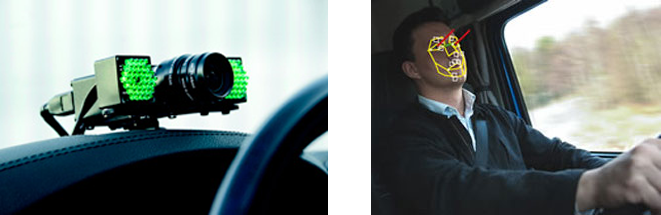
\includegraphics[width=140mm, keepaspectratio]{figures/driving.png}
\caption{\textbf{Bal:} A \emph{Daimler} tekintetkövető kamerája. \\ Forrás: \url{http://bit.ly/14jX6I2} \\
\textbf{Jobb:} A \emph{Seeing Machines} DSS fantázianevű megoldása. \\ Forrás: \url{http://bit.ly/16HLaDE}}
\label{fig:driving}
\end{figure}

%,,,,,,,,,,,,,,,,,,,,,,,,,,,,,,,,,,,,,,,,,,,,,,,,,,,,,,,,,,,,,,,,,,,,,,,,,,,,
\section{Összefoglalás}\label{sect:felh_osszefoglalas}
%,,,,,,,,,,,,,,,,,,,,,,,,,,,,,,,,,,,,,,,,,,,,,,,,,,,,,,,,,,,,,,,,,,,,,,,,,,,,

A fejezetben bemutatott kutatási és gyakorlati felhasználási lehetőségek, problémák felsorolásával éppen csak a felszínét érintettem azon területek, részproblémák halmazának, amelyek körében a tekintetkövetés potenciálisan felhasználható lehet.

Való igaz, hogy a dolgozatom írásakor is már több, különféle elveken (összefoglalásukat lásd a \sectref{tekintetkovetes} fejezetben) működő rendszer megtalálható egyetemi laborokban, illetve a piacon. Azonban amint említettem, maga a terület, és az egyes projektek anyagi lehetőségei is annyira szerteágazóak, hogy mindenképpen igény mutatkozik egy főleg képfeldolgozással operáló -- azaz komoly hardverköltségek nélküli -- tekintetkövető rendszer fejlesztésére.
%----------------------------------------------------------------------------
\chapter{A tekintetkövetésről}\label{sect:tekintetkovetes}
%----------------------------------------------------------------------------

A tekintetkövető rendszer fejlesztésének megkezdése előtt számos elméleti és gyakorlati szempont veendő figyelembe, hogy a rendszer által nyújtott kritériumok a lehető legjobban közelítsék az elvártat. Nem kerülhető meg az általános technikák, vagy már meglévő megoldások áttekintése a szakirodalomból, aminek segítségével képet alkothatunk a kutatási téma jelenlegi állásáról, és a gyakorlati szempontok figyelembe vételével dönthetjük el, hogy mely módszer mellett tesszük le végül a voksunkat.

\bigskip

A fejezet \sectref{modszerek} szakaszában mindenekelőtt a jelenleg elérhető tekintetkövetési módszereket veszem górcső alá, majd hasonlítom össze őket, hogy kellően megalapozott döntést hozhassak a később felhasználni kívánt technikával kapcsolatban. 

%,,,,,,,,,,,,,,,,,,,,,,,,,,,,,,,,,,,,,,,,,,,,,,,,,,,,,,,,,,,,,,,,,,,,,,,,,,,,
\section{Tekintetkövetési módszerek}\label{sect:modszerek}
%,,,,,,,,,,,,,,,,,,,,,,,,,,,,,,,,,,,,,,,,,,,,,,,,,,,,,,,,,,,,,,,,,,,,,,,,,,,,

Bár már lassan másfél évtizedes, a témában mégis hiánypótló munka Arne John Glenstroupnak és Theo Engell-Nielsennek, a dán Københavns Universitet (Koppenhágai Egyetem) hallgatóinak diplomamunkája \cite{eye_media}. Dolgozatuk jelen szempontból fontos második fejezetét a modern tekintetkövetési technikák bemutatásának és összehasonlításának szentelik, meglátásaik pedig mind a mai napig helytállóak.

\bigskip

Ebben a szakaszban főleg az ő munkájuk alapján szeretném összefoglalni a tekintet követésére felhasználható technikákat, néhol a lényeg kiemelésével, ahol pedig szükséges, a hivatkozott cikk keletkezése óta az idő múlásával érvénytelenné vált adatok, paraméterek aktualizálásával.

%............................................................................
\subsection{Az ideális tekintetkövető}\label{sect:idealis}
%............................................................................

Manapság számos módszer kínálkozik a tekintet követésére. De mégis milyen követelményeket kell teljesíteni az ,,ideális'' tekintetkövetőnek? Scott és Findlay 1993-as munkájukban \cite{scott} Hallett eredményeit \cite{hallett} figyelembe véve meghatározták az ideális tekintetkövető eszköz (vagy rendszer) paramétereit és tulajdonságait.

Ezek szerint az ideális tekintetkövető eszköznek a következő 12 pont által támasztott követelményeket kell teljesítenie:

\begin{enumerate}[a.]
 \item az arc és a fejrégió könnyen hozzáférhető maradjon
 \item ne legyen fizikailag kapcsolatban a vizsgált személlyel
 \item ha szükséges, képes legyen stabilizálni a kapott eredményeket
 \item a rendszer \emph{pontossága} néhány százalékos (1--2 szögperces) eltérést engedjen meg
 \item támogasson legalább egy szögperces \emph{felbontást} másodpercenként, hogy a szempozíció legkisebb változása is követhető legyen; a felbontásnak csak az érzékelő eszköz zaja szabjon határt
 \item támogasson kellően széles \emph{dinamika-tartományt} a szem mozogásainak leképezéséhez
 \item a rendszer időbeli dinamikája legyen megfelelő (jó erősítés, kis fázistolás)
 \item nyújtson \emph{valósidejű} válaszidőt
 \item legyen \emph{invariáns} mindhárom forgási és eltolási szabadságfokra
 \item egyszerűen kiterjeszthető legyen mindkét szem feldolgozására (\emph{binokuláris} vizsgálat)
 \item \emph{kompatibilis} meglévő legyen fej- és testfelvételek használatával
 \item tesztalanyok széles skáláján (pl. nem, kor, rassz szerint, vagy szemüvegesek és szemüveg nélküliek körében) használható legyen
\end{enumerate}

A fent felsorolt követelmények valóban az ideális esetet testesítik meg. Sokszor egy követelmény enyhítésével, vagy figyelmen kívül hagyásával más követelmények kielégítése jelentősen egyszerűsödik. Ha például a \emph{b.} pont szerinti fizikai kontaktust mégis megengedjük, rögzíthetjük a követésre használt kamerát a vizsgálni kívánt alany fejéhez (természetesen kellően diszkrét és kényelmes módon). Ebben az esetben a \emph{i.} pont szerinti invariancia biztosítása máris egyszerűbb feladat, mint külső nézőpontból geometriai transzformációk segítségével végezni ugyanezt.

Több más, látszólag egymásnak ellentmondó követelményt is észrevehetünk az ideális tekintetkövető eszköz 12 pontja között. Komoly megoldandó mérnöki feladatot jelent az ütközések feloldásával az ideális eszközt különböző, valós életben használható megoldásokká alakítani.

\bigskip

A gyakorlatban használható tekintetkövetési megoldások egy lehetséges csoportosítása az alábbi elveken működő iránymeghatározásokat tartalmazza:

\begin{enumerate}
 \item a szem felületének (vagy a felület speciális megvilágításának) alapján, optikai elven 
 \item a szem körüli bőrfelület elektromos potenciáljának mérésével
 \item speciális kontaktlencse használatával
\end{enumerate}

Már csekély megfontolással látszik, hogy minden csoportnak vannak előnyei és hátrányai. Például az \emph{1.} csoportba tartozó megoldások igénylik a legkevésbé -- többnyire egyáltalán nem -- a fizikai kontaktust a vizsgált személlyel. Azonban elképzelhető, hogy ennek az az ára, hogy az ebbe a csoportba tartozó megoldások nem veszik fel a versenyt a másik két alapelv szerint fejlesztett rendszerekkel pl. a pontosság, vagy valamely más kritérium tekintetében.

Ennek megfelelően szükség van a lehetőségek számba vételére, értékelésére, majd összehasonlítására, hogy a legmegfelelőbb technikát tudjuk kiválasztani, ha tekintetkövető eszköz (alkalmazás) fejlesztésébe fogunk. A következő szakaszokban ezért röviden ismertetem a fenti kategóriákba eső megoldások alapjait, majd összehasonlítom jellemző tulajdonságaikat, valamint a használatukkal elérhető fontos pontossági- és sebességértékeket.

%............................................................................
\subsection{Optikai elvű követés}\label{sect:optikai}
%............................................................................

Az optikai elvű követés során -- a nevéből adódóan -- optikai úton próbáljuk meghatározni a tekintet irányát. Ez történhet speciális megvilágítás nélkül, pl. az írisz (pontosabban az írisz és az ínhártya közti határvonal, a limbus), vagy a pupilla követésével.

A másik lehetséges megoldásra a szem speciális, többnyire infravörös fénnyel történő megvilágítása, majd a szemgolyó felületén megjelenő tükröződések, visszaverődések vizsgálata kínálkozik. Az infravörös megvilágítás előnye a látható fénnyel szemben egyrészt az, hogy nem zavarja a vizsgált személyt, nem vonja el a figyelmét, másrészt pedig infraszűrők használatával a látható fény tartományába eső változásokkal a megfelelő körülmények között (lehetőleg kevés napfény a magas infratartalma miatt) invariánssá tehető.

%. . . . . . . . . . . . . . . . . . . . . . . . . . . . . . . . . . . . . .
\subsubsection{Limbuskövetés}\label{sect:limbusz}
%. . . . . . . . . . . . . . . . . . . . . . . . . . . . . . . . . . . . . .

Az írisz és az ínhártya közötti határvonal a többnyire nagy intenzitásváltozás miatt könnyen detektálható lehet. Ugyanakkor meg kell jegyeznünk, hogy az esetek jelentős részében a limbus számottevő része lehet a szemhéjak takarásában. Ennek megfelelően a technika csak vízszintes helyzet és mozgás követésére alkalmas kielégítő pontossággal \cite{scott}.

Klasszikus esetben ez a követési technika a limbus \emph{relatív} fejhez képest helyzetén alapul, ezért a vizsgálat közben a fejmozgások teljes hanyagolását, esetleg a tekintetkövető eszköz fejhez rögzítettségét igényli.

%. . . . . . . . . . . . . . . . . . . . . . . . . . . . . . . . . . . . . .
\subsubsection{Pupillakövetés}\label{sect:pupilla}
%. . . . . . . . . . . . . . . . . . . . . . . . . . . . . . . . . . . . . .

A pupillakövetési technika hasonló az előbb említett limbuskövetéshez, de némi többlet előnyt is magában hordoz. Az egyik ilyen előny, hogy a pupilla közel sincs olyan nagy részben a szemhéjak takarásában, mint a limbus, ennek következtében függőleges irányú követés is megvalósítható lehet. A másik előny, hogy az írisz és a pupilla közti határvonal jóval élesebb, mint az írisz-ínhártya határa, ezért jobb felbontással, pontosabban tudjuk meghatározni a nézeti irányt.

Az előző technikához képest azonban meg kell említeni a felmerülő nehézségeket is. A kontraszt ugyan lehet, hogy nagyobb az írisz-pupilla határon, azonban az intenzitáskülönbség nem olyan jelentős, mint a limbus környezetében. Az sem elhanyagolható szempont, hogy a pupilla átmérője is szükségszerűen kisebb, mint az íriszé, vagyis a forrásnak relatívan nagyobb felbontásúnak kell lennie, hogy azonos pixelnyi méretű pupillát és íriszt detektálhassunk; ellenkező esetben a kisebb abszolút méret a pontosság rovására mehet.

%. . . . . . . . . . . . . . . . . . . . . . . . . . . . . . . . . . . . . .
\subsubsection{Visszaverődés-alapú követés}\label{sect:visszaverodes}
%. . . . . . . . . . . . . . . . . . . . . . . . . . . . . . . . . . . . . .

A szemet (infravörös) fénnyel megvilágítva több tükröződés is megfigyelhető lesz a szemlencse és a szaruhártya határán: ezek az úgynevezett \emph{Purkinje-képek} (lásd \figref{purkinje} ábra).

\begin{figure}[!ht]
\centering
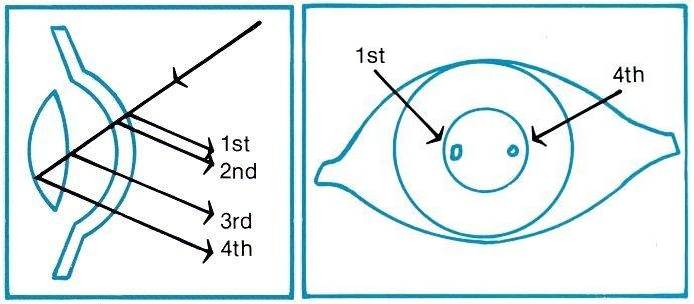
\includegraphics[width=110mm, keepaspectratio]{figures/purkinje_kepek.png}
\caption{A \emph{Purkinje-képek} elhelyezkedése. Forrás: \url{http://bit.ly/YnAowY}}
\label{fig:purkinje}
\end{figure}

Ezen visszavert képek intenzitása sorrendben egyre csökken, az első azonban (közkeletű nevén az úgynevezett \emph{,,csillanás''}, angolul \emph{glint}) még viszonylag egyszerűen detektálható. Infravörös megvilágításban ugyancsak egyszerű a megfelelő kamerával a pupilláról visszavert fény detektálása -- a pupilla a környezeténél jóval nagyobb mértékben veri vissza az infravörös fényt, az infraképen egy ,,fényes'', kontrasztos objektumot alkotva.

A fenti két objektum egymáshoz viszonyított \emph{relatív} helyzetéből következtethetünk a tekintet irányára, ugyanis az első Purkinje-kép világos pontja, illetve a pupilla kontrasztos ellipszise egymással összefüggésben mozdulnak el a fej vagy a szem mozgatásának következtében.

Az előző bekezdésben foglaltakból látszik, hogy a technika nem igényeli a fej mozdulatlanságát, vagy a képfelvevő eszköz fejhez rögzítését. Ezen előnye azonban egy megkötést is magával hordoz: egyszerű algoritmusok segítségével kb. $\pm12$--$15$ foknyi szabadsága van a felhasználónak a fejmozgásokra \cite{scott}, nagyobb mértékű mozgások esetén ugyanis komplexebb matematikai számítások szükségesek a követett objektumok mozgásának modellezéséhez.

\bigskip

A visszaverődés-alapú megoldásokkal rokonítható még az a módszer, amikor szintén az első Purkinje-kép erős visszaverődését detektálva a képen, kivágunk egy viszonylag kicsi (párszor tíz pixel nagyságrendű) részt, a csillanással a középpontban. Az így kapott képről egy neurális hálózat dönti el, hogy milyen nézeti irányhoz tartozik \cite{baluja}.

A neurális hálózatot természetesen be kell tanítani a használhatóság érdekében. A betanítási procedúra első lépéseként tanítóképeket kell generálni, általános esetben pár percet vesz igénybe, ami alatt a követnie kell egy, a képernyőn megjelenő jelzést. A tanítóképek birtokában ezután a hálózat betanítható, ez a jelenlegi technikai szint mellett kb. tíz perces nagyságrendű időt vesz igénybe. Azonban azonos körülmények és tesztszemély esetén a tanítást nem kell máskor újra elvégezni.

A neurális hálózat előnye a betanítás után, használat közben mutatkozik meg leginkább: felépítéséből adódóan a háló nagyon rövid idő alatt ,,döntést tud hozni'', így a valósidejű feldolgozási sebesség kritériuma mindenképpen kielégített lesz. A döntés eredménye ráadásul akár közvetlenül felhasználható: mindössze úgy kell megterveznünk a rendszert, hogy a neurális háló kimenet közvetlenül egy kétdimenziós koordinátát szolgáltasson a felhasznált képernyő koordináta-rendszerében.

A módszer egy másik előnye, hogy nem igényel közeli, nagy felbontású képet a szemrégióról, egy átlagos felbontású kamerával, pl. kartávolságból is elegendő nagyságú lesz a szemrégió. Ennek egyik folyományaként -- hogy nagyobb látószögű képek használhatók -- adódik, hogy viszonylag nagy mozgási szabadsága lehetséges a vizsgált személy fejének tekintetében, anélkül, hogy a kamerát újra kéne pozicionálnunk.

Ennek a szabadságnak azonban ára van: ha a kalibrálási fázis során több fejpozícióból is rögzítettünk tanító képeket, akkor a betanítás után a neurális hálózat jó eséllyel fogja felismerni különböző fejpozíciókban is a tekintet irányát; a mozgási szabadság azonban a pontosság csökkenésével jár. A pontosság egyébként is érzékeny pontja az eljárásnak, ezt pedig éppen úgy növelhetjük, ha tanítás és előhívás közben \emph{nem} engedjük meg, hogy a fejpozíció változzon.

%. . . . . . . . . . . . . . . . . . . . . . . . . . . . . . . . . . . . . .
\subsubsection{Purkinje-képek követése}\label{sect:purkinje}
%. . . . . . . . . . . . . . . . . . . . . . . . . . . . . . . . . . . . . .

Egy további lehetséges optikai elven működő tekintetkövetési technikát mutatott be Müller \emph{et al} 1993-ban \cite{muller}, \emph{,,Kettős Purkinje-kép''} (Dual-Purkinje Image) módszer néven. Az eljárás lényege, hogy a már említett első és negyedik Purkinje-kép egymáshoz viszonyított helyzetéből számítja a tekintet irányát. Megfelelő matematikai modell esetén a módszer rendkívül pontos, azonban a negyedik Purkinje-kép alacsony intenzitása miatt hatványozottan érzékeny a megvilágítási problémákra.

%............................................................................
\subsection{Elektromos potenciál-alapú követés}\label{sect:potencial}
%............................................................................

Az eddigiektől egy merőben eltérő megközelítése a problémának az \emph{elektro-okulográfia} (EOG). Az eljárásból nyerhető elektro-okulogram rögzítése pl. megismerési és kognitív folyamatok, a vizuális információfeldolgozás, vagy az alvásvizsgálat terén szokásos.

\begin{figure}[!ht]
\centering
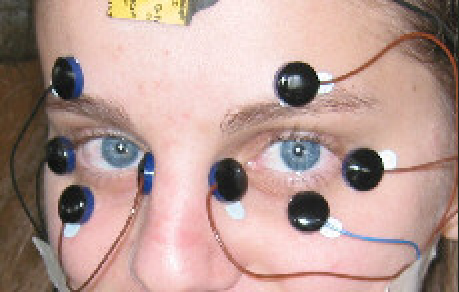
\includegraphics[width=80mm, keepaspectratio]{figures/eog.png}
\caption{Az EOG eljárás elektródái. Forrás: \url{http://bit.ly/13a7IcL}}
\label{fig:eog}
\end{figure}

A módszer a szemgolyó elülső és hátulsó pólusa közötti potenciálkülönbség mérésén alapul, amellyel mind függőleges, mind vízszintes irányban követhető a szem mozgása, de csak körülbelül $1$--$2$ fok pontossággal. A használata azonban korántsem mondható egyszerűnek: az potenciálváltozást érzékelő elektródák (lásd \figref{eog}) miatt szükséges fizikai kontaktuson kívül a rendszer kalibrációja rendkívül hosszadalmas, és hozzáértést igénylő feladat.

%............................................................................
\subsection{Követés speciális kontaktlencse használatával}\label{sect:kontakt}
%............................................................................

A szem helyzetének, ebből közvetve a tekintet irányának számításához speciális kontaktlencséket is használhatunk. Az egyik lehetséges megoldás, hogy a lencse anyagában olyan véseteket alakítanak ki (tipikusan valamilyen könnyen felismerhető mintázatot), amelyek a fénytörés felhasználásával megkönnyítik a szem helyzetének meghatározását.

Ha azonban egy megfelelően kis méretű indukciós tekercset is sikerült a kontaktlencse anyagába ágyazni, akkor a fej körül generált nagyfrekvenciás elektromágneses mezőkkel az tekercs helyzete közvetlenül is könnyen meghatározható. Az eljárás körülményessége azonban kétségessé teszi a technika laboratóriumokon kívüli felhasználását.


%............................................................................
\subsection{A tekintetkövetési módszerek összehasonlítása}\label{sect:tekintet_osszehas}
%............................................................................

A \tabref{osszehas} táblázat tartalmazza az ebben a szakaszban felsorolt tekintetkövetési módszerek összehasonlítását. Az összehasonlítás szempontjai a módszer által igényelt kontaktust, az általa nyújtott pontosságot, illetve felbontást (hogy a bemeneti képen mekkora minimális elmozdulás jelent változást a kimeneti pozícióban) jelentik. 

\begin{table}[ht]
	\centering
	\caption{A felsorolt tekintetkövetési módszerek összehasonlítása.} \label{tab:osszehas}
	\begin{tabular}{ l || c | c | c | c | c | c | c }
	 & kontaktus & pontosság & felbontás \\ \hline \hline
	limbuskövetés & pl. áll-tartó & $1$--$7^\circ$ & $0,\!1^\circ$ \\
	pupillakövetés & nincs & $0,\!003^\circ$ & $0,\!005^\circ$ \\
	visszaverődés alapú & nincs & $0,\!5$--$2^\circ$ & jó \\
	neurális hálózat & nincs & $1,\!5\circ$ & -- \\
	kettős Purkinje-képek & nincs & $0,\!017^\circ$ & $0,\!25^\circ$ \\ 
	elektro-okulográfia & elektródák & $\pm1,\!5$--$2^\circ$ & jó \\
	kontaktlencse & kontaktlencse & $0,\!08^\circ$ & $0,\!017^\circ$ \\
	\end{tabular}
\end{table}

%----------------------------------------------------------------------------
\section{Szemmozgások}\label{sect:osztalyozas}
%----------------------------------------------------------------------------

%\begin{verse}
%\begin{flushright}
%\emph{A szív érez, a szem kutat} \\
%\dots
%\end{flushright}
%\end{verse}

A szemmozgások többsége -- így a későbbi vizsgálatok szempontjából fontosak is -- a retinán elhelyezkedő sárgafolt (\emph{fovea centralis}, lásd \figref{eyediag} ábra) helyzetének megváltoztatására szolgál. A látóideg kivezetése mellett elhelyezkedő sárgafolton csak tömötten egymás mellé rendeződött csapok találhatók. A csapok jó fényviszonyok mellett nagyon magas felbontásban képesek színek gazdag skáláját feldolgozni, ezért a legélesebb látás a sárgafoltra vetített kép esetén lehetséges. Érthető tehát, hogy a sárgafoltot olyan pozícióba célszerű mozgatni, hogy a figyelem tárgyának képe ide vetüljön. Az ehhez szükséges pozicionáló típusú szemmozgások közé tartoznak a \emph{szakkádok}, a \emph{lassú követések}, és -- bár meglepőnek tűnik -- a \emph{fixációk} is, ezekkel a fejezet további szakaszaiban részletesebben foglalkozok.

\begin{figure}[!ht]
\centering
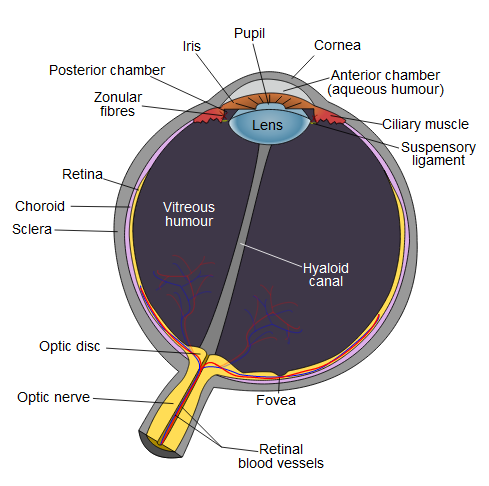
\includegraphics[width=100mm, keepaspectratio]{figures/eye_diagram.png}
\caption{Az emberi szem felépítése. Forrás: \url{http://en.wikipedia.org/wiki/Eye}}
\label{fig:eyediag}
\end{figure}

A \emph{fovea} pozicionálását elősegítő mozgások mellett természetesen más is szerepet kap a kívánt kép előállításában. A teljesség igénye nélkül, ilyenek például a szem divergenciáját illetve konvergenciáját beállító mozgások (mélységérzékelés), valamint azok a reflexszerű mozgások, amelyek az egyensúlyszervvel összhangban beállítják a szemeket a fej térbeli orientációjának megfelelően.

\bigskip

A szakasz első részében sorra veszem, és bemutatom a pozicionáló típusú szemmozgások alapjait, a mérnöki megközelítésből jelentéktelen részleteket mellőzve. Végül a \sectref{mozg_osszegzes} szakaszban összefoglalom a megszerzett ismereteket, valamint hogy a megismert mozgások milyen követelményeket, illetve korlátozásokat támasztanak a realizálandó rendszer tervezése során.

%,,,,,,,,,,,,,,,,,,,,,,,,,,,,,,,,,,,,,,,,,,,,,,,,,,,,,,,,,,,,,,,,,,,,,,,,,,,,
\subsection{Szakkádok}\label{sect:szakkadok}
%,,,,,,,,,,,,,,,,,,,,,,,,,,,,,,,,,,,,,,,,,,,,,,,,,,,,,,,,,,,,,,,,,,,,,,,,,,,,

A szakkád mindkét szem gyors, egyidejű, azonos irányú mozgását jelenti. Célja a fixáció áthelyezése az egyik tárgyról a másikra. A mozgás során észlelt jellegzetes ,,ugráló'' mintáról kapta a nevét: a francia \emph{saccader} szó jelentése ,,rángatás'', ,,ugrás''.

A szakkádok lehetnek akaratlagosak és reflexszerűek is. Az egyensúlyszervből érkező jelre például reflexszerűen aktiválódhatnak, míg a tekintetünk, figyelmünk áthelyezése nyilvánvalóan akaratlagos cselekedet. Időtartamban a szakkádok körülbelül 10 és 100~ms közé tehetők. Ez kellően rövid ahhoz, hogy az agy a gyakorlatban ne észlelje, hogy a mozgás alatt nem történik információfelvétel -- vagyis a szakkádikus mozgás közben pár pillanatra effektíve vakok vagyunk. \cite{shebilske}

A szakkádok végrehajtásáról megoszlanak a vélemények. Korábban a szakkádokat ballisztikusnak tartották, vagyis amint a következő fixációs pont helye kiszámításra kerül (nagyjából 200~ms idő alatt), a mozgás már nem megszakítható vagy megváltoztatható. \cite{carpenter_book} Ezt a feltevést támasztotta alá a tény, hogy a végrehajtás 10-100~ms-os időtartama alatt vizuális visszacsatolásra nincs elegendő idő. Léteznek feltevések azonban, amelyek szerint nincs szükség vizuális visszacsatolásra a végrehajtás közbeni megváltoztatáshoz, így a mozgás ballisztikussága (a nagy sebességek miatt) csak látszólagos. \cite{zee}

%,,,,,,,,,,,,,,,,,,,,,,,,,,,,,,,,,,,,,,,,,,,,,,,,,,,,,,,,,,,,,,,,,,,,,,,,,,,,
\subsection{Lassú követések}\label{sect:lassukovetes}
%,,,,,,,,,,,,,,,,,,,,,,,,,,,,,,,,,,,,,,,,,,,,,,,,,,,,,,,,,,,,,,,,,,,,,,,,,,,,

A lassú követés (\emph{smooth pursuit}) mozgó tárgyak vizuális követésére szolgál. Az ilyen típusú mozgás könnyen modellezhető egy negatív visszacsatolású szabályozóval. \cite{carpenter_book}

Egy bizonyos sebességig a szem képes tisztán lassú követést használni a fixáció tárgyon tartására, azonban a 30$^{\circ}$/s sebességnél gyorsabban mozgó tárgyak esetén a megfelelő követéshez általában szakkádok beiktatása szükséges. Itt jegyzendő meg, hogy a lassú követés vízszintes és függőleges irányban nem szimmetrikus: a legtöbb ember a vízszintes mozgásokat jobban, míg a függőleges mozgásokat kevésbé tudja lekövetni (ahol ,,jó'' követésen azt értjük, hogy nem szükséges szakkádok beiktatása). A szakkádokkal ellentétben a lassú követést egyértelműen megváltoztathatja az érzékelt vizuális visszacsatolás, a mozgás nem ballisztikus.

Érdekesség, hogy a legtöbben vizuális stimuláció (tényleges mozgó tárgy) nélkül nem tudnak lassú követéses szemmozgást előidézni, csak rövid szakkádok gyors egymásutánját. Szintén megemlítendő, hogy a lassú követés bár hasonlónak tűnik ahhoz, amikor a fej mozgását ,,kompenzálva'' egy álló tárgy képét fixáljuk a látómezőn, a két mozgás alapvetően különbözik: már abban is, hogy míg az egyik akaratlagos, a másik reflexszerűen hajtódik végre.

%,,,,,,,,,,,,,,,,,,,,,,,,,,,,,,,,,,,,,,,,,,,,,,,,,,,,,,,,,,,,,,,,,,,,,,,,,,,,
\subsection{Fixációk}\label{sect:fixaciok}
%,,,,,,,,,,,,,,,,,,,,,,,,,,,,,,,,,,,,,,,,,,,,,,,,,,,,,,,,,,,,,,,,,,,,,,,,,,,,

A fixációs mozgások a retina stabilizálására szolgálnak, aminek köszönhetően az álló objektumokat tudjuk figyelmünk középpontjában tartani. Az előző szakasz alapján azt gondolhatnánk, hogy a fixációt ugyanazok az idegi pályák aktiválhatják, mint amelyek a lassú követésért felelősek, mindössze a ,,mozgás'' sebessége zérus.

A fixáció azonban több, mint nulla sebességű mozgás: a fixációk közben \emph{tremor}, \emph{drift} és \emph{mikroszakkád} jellegű mozgások váltják folyamatosan egymást. Az állandó mozgást a fényérzékelő sejtek felépítése indokolja. Ha a kép pár másodpercnél tovább marad teljesen változatlanul a retinán, a sejtek telítésbe kerülnek, és a tekintet elhomályosul.

%,,,,,,,,,,,,,,,,,,,,,,,,,,,,,,,,,,,,,,,,,,,,,,,,,,,,,,,,,,,,,,,,,,,,,,,,,,,,
\subsection{Nystagmus}\label{sect:nystagmus}
%,,,,,,,,,,,,,,,,,,,,,,,,,,,,,,,,,,,,,,,,,,,,,,,,,,,,,,,,,,,,,,,,,,,,,,,,,,,,

A nystagmus szakkádok és lassú követések egymásutánja, nem akaratlagos szemmozgás. Előidéződhet optokinetikus úton, illetve patológiásan is (pl. kábítószer-használat hatására). Patológiás nystagmus jelenléte orvosi szempontból lehet jóindulatú, de akár mélyebb neurológiai problémákra is utalhat.

%,,,,,,,,,,,,,,,,,,,,,,,,,,,,,,,,,,,,,,,,,,,,,,,,,,,,,,,,,,,,,,,,,,,,,,,,,,,,
\subsection{Összegzés}\label{sect:mozg_osszegzes}
%,,,,,,,,,,,,,,,,,,,,,,,,,,,,,,,,,,,,,,,,,,,,,,,,,,,,,,,,,,,,,,,,,,,,,,,,,,,,

A fejezet első szakaszában röviden bemutattam a \emph{fovea} pozicionálására szolgáló szemmozgásokat, amelyek alapszintű megismerése elengedhetetlen a tekintetkövető rendszer fejlesztése során. A rendszernek -- ahogy ez a mozgások tulajdonságaiból kitűnik -- mind a gyorsaság, mind a pontosság tekintetében komoly követelményeket kell teljesítenie.

Az elérendő \textit{gyorsasághoz} a szakkádok, mint a leggyorsabb sebességű mozgások időtartama (10-100~ms) adhat támpontot. Egy átlagos kamerakép 60~Hz-es frissítése legjobb esetben 16~ms időközönkénti vizsgálatot tesz lehetővé. Ez az eredmény egy tipikus drágább, digitális webkamera 30 képkocka/másodperces képfrissítésével máris 33~ms-ra csökken, nem is beszélve a 30~FPS-nél gyengébb teljesítményű kamerákról. Tisztában kell lennünk tehát azzal, hogy átlagos képrögzítő hardver használatával előfordulhat olyan szituáció, hogy fizikailag képtelenek vagyunk a nagyon gyors szakkádok pontos követésére.

A \textit{pontosság} tekintetében azt kell figyelembe vennünk, hogy (pl. olvasásnál) a két egymást követő fixációs pont közti eltérés akár szögperces nagyságrendű is lehet. Ezek korrekt elkülönítéséhez nyilvánvalóan minél nagyobb felbontás szükséges. Minél kisebb felbontásúak a felvételek (azaz a szem, illetve a pupilla megjelenítésére relatíve kevesebb képpont kerül), annál nagyobb elmozdulás jut egyetlen képpontra, ami a feldolgozás során a legkisebb elkülöníthető egység.


%,,,,,,,,,,,,,,,,,,,,,,,,,,,,,,,,,,,,,,,,,,,,,,,,,,,,,,,,,,,,,,,,,,,,,,,,,,,,
\section{Optikai megfontolások}\label{sect:hw_optikai}
%,,,,,,,,,,,,,,,,,,,,,,,,,,,,,,,,,,,,,,,,,,,,,,,,,,,,,,,,,,,,,,,,,,,,,,,,,,,,

Az optikai megfontolások közül az első a tekintetkövetés során felhasznált fénytartomány, ami lehet a látható fény tartománya, valamint az infratartomány. A második fontos szempont pedig a kamera látószöge, ami alapjaiban határozza meg a felhasználótól megkívánt beavatkozás mértékét, valamint a szem felbontását (ezzel közvetve az elérhető maximális pontosságot).

\bigskip

A \textbf{látható fényben} történő követés egyértelmű előnye, hogy nem igényel speciális hardvert, a legtöbb, a piacon kapható analóg vagy digitális (web)kamera ebben a tartományban ,,lát''. Sőt, a digitális eszközökben a CMOS/CCD érzékelő elé szinte minden esetben ún. infratükröt (felülvágó szűrőt, amely kirekeszti a látható fény feletti spektrumot) helyeznek, ezeket az eszközöket tehát sikerrel csak látható fényben használhatjuk. A látható fény használatakor azonban nem feledkezhetünk meg annak hátrányairól sem: a követéshez analizálandó kép meglehetősen érzékeny lesz a megfelelő megvilágításra. A fényviszonyok változásának kiküszöbölése komolyabb előfeldolgozást kíván, és extrém esetekben nem is mindig teljesíthető.

\begin{figure}[!ht]
\centering
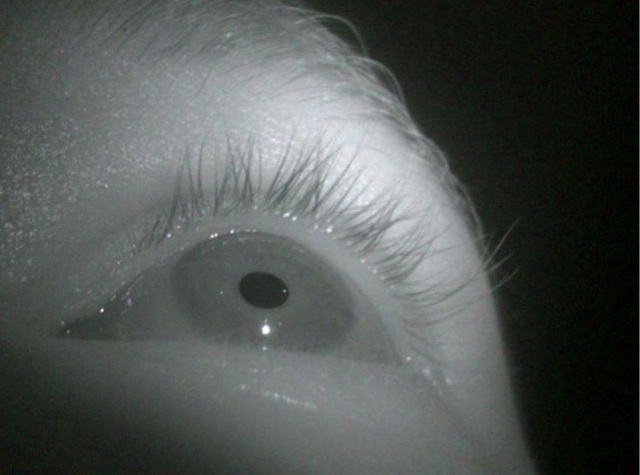
\includegraphics[width=100mm, keepaspectratio]{figures/infra_eye.png}
\caption{Az emberi szem képe infravörös fényben. Forrás: \url{http://bit.ly/aKwzsZ}}
\label{fig:eyepic}
\end{figure}

Az \textbf{infratartománynak} a látható fénnyel szemben vannak előnyei, és hátrányai is. Az előnyök közé tartozik, hogy a pupilla képe a infra megvilágításban nagyon kontrasztos (lásd \figref{eyepic} ábra), jóval könnyebben szegmentálható az írisztől (különösen sötétebb szemű alany esetén), mint látható fényben. Az infrás megvalósítás hátránya azonban, hogy a megfelelő működéshez sötétet igényel (igaz, ezzel összhangban a látható megvilágítási változásokra invariáns), de sötétben, a tisztán infra megvilágítás megvalósítása nehéz feladat, különösen a piacon kapható egyszerűbb infra LED-ekkel, vagy LED-es reflektorokkal.

\bigskip

A követéshez használt kamera optikája lehet egyrészt \textbf{nagylátószögű}. Ez azzal az előnnyel jár, hogy a vizsgálat alatt álló személy fejmozgása szabadabb lehet, nincs szükség a fejpozíció fixálására (pl. álltámasszal). A szemrégió külön szegmentálható, majd ezen régión belül a pupillát követve valósulhat meg a tekintetkövetés. A módszer hátránya, hogy a szemrégió nem tölti be az egész képet, vagyis nem használja ki maximálisan a rendelkezésre álló felbontást. Ennek következtében a tekintetkövetés pontossága jelentős mértékben romolhat, esetleg lehetetlenné is válhat.

További lehetőség a \textbf{teleobjektívek}, vagyis zoomoptikák használata. Teleobjektívvel a szemrégió ,,közel hozható'' még nagy távolságról is, hogy teljesen kitöltse a feldolgozandó képet, kihasználva annak teljes felbontását. Ez azonban azzal a hátránnyal jár, hogy a fejet fix pozícióba kell kényszeríteni (pl. egy álltámasz segítségével), ugyanis a fej mozgásával a pupillarégió kikerülhet a kamera látószögéből.

Végül lehetőség nyílik egyfajta ,,hibrid'' megoldás használatára is, amelynél a két megoldás előnyeit ötvözhetjük.
%----------------------------------------------------------------------------
\chapter{Elméleti alapok}\label{sect:elmeleti_alapok}
%----------------------------------------------------------------------------

Már a szakdolgozatomban \cite{thesis_sajat} is arra kerestem a választ, hogy melyek lehetnek a pupilla követésének gyors és robusztus megvalósításai. A kérdés a tekintetkövető rendszer esetében is kardinális: a pupilla gyors és pontos követése a elengedhetetlen a megfelelő minőségű követés megvalósításához.

Munkám során számos módszer elméletét kellett megértenem, majd a gyakorlatba ültetnem. Dolgozatomnak ebben a fejezetében ezért a legfontosabb általam vizsgált módszerek alapjaival szeretném megismertetni az olvasót.

\bigskip

A \sectref{hough} szakaszban a Hough-transzformációt mutatom be, kitérve a pupillakeresés szempontjából fontos körkeresési probléma megoldására. A fejezet \sectref{objdetect} szakaszában az objektumdetektálás és -követés lehetőségének elméletét ismertetem a Viola--Jones objektumdetektor és a Lucas--Kanade optikai áramlás módszerein keresztül. Végezetül a blob-alapú követés alapjait jelentő blobok felismerésével és szűrésével kapcsolatos tudnivalókat foglalom össze a \sectref{blob} szakaszban.

%,,,,,,,,,,,,,,,,,,,,,,,,,,,,,,,,,,,,,,,,,,,,,,,,,,,,,,,,,,,,,,,,,,,,,,,,,,,,
\section{Hough-transzformáció}\label{sect:hough}
%,,,,,,,,,,,,,,,,,,,,,,,,,,,,,,,,,,,,,,,,,,,,,,,,,,,,,,,,,,,,,,,,,,,,,,,,,,,,

Képfeldolgozási szűrők, függvények segítségével viszonylag könnyen előállíthatjuk a képtérben számunkra érdekes pontok halmazát. Azokat a pontokat, amelyek valamilyen magasabb absztrakciós szintű képjellemzőhöz kapcsolódnak: például a tárgyak, alakzatok formáját megadó kontúrok pontjait. Ha viszont szeretnénk ,,megérteni'' is a képet, az ilyen formák automatikus és robusztus felismerése szinte elengedhetetlen.

A valóságban a kontúrok pontjai azonban csak többé-kevésbé illeszkednek ideális formákra (egyenesekre, körökre, vagy egyéb görbékre): az éleket torzíthatja zaj, egyes élpontok hiányozhatnak, vagy a felismerni kívánt formák kismértékben el is térhetnek az ideálistól. A kép analízise szempontjából azonban ezzel együtt is nagyon értékes információt rejthetnek magukban, ezt az információt pedig hasznos lenne kinyerni. Viszont egyáltalán nem triviális probléma a valamilyen szempontból összetartozó (például egy egyenesre, vagy egy körvonalra eső) pontok csoportosítása.

\begin{figure}[!ht]
\centering
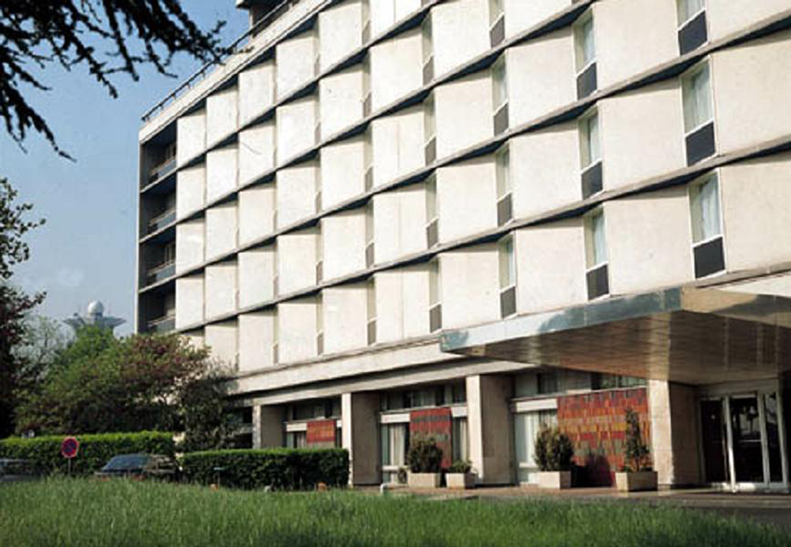
\includegraphics[width=67mm, keepaspectratio]{figures/houghline_building_1.png}\hspace{1cm}
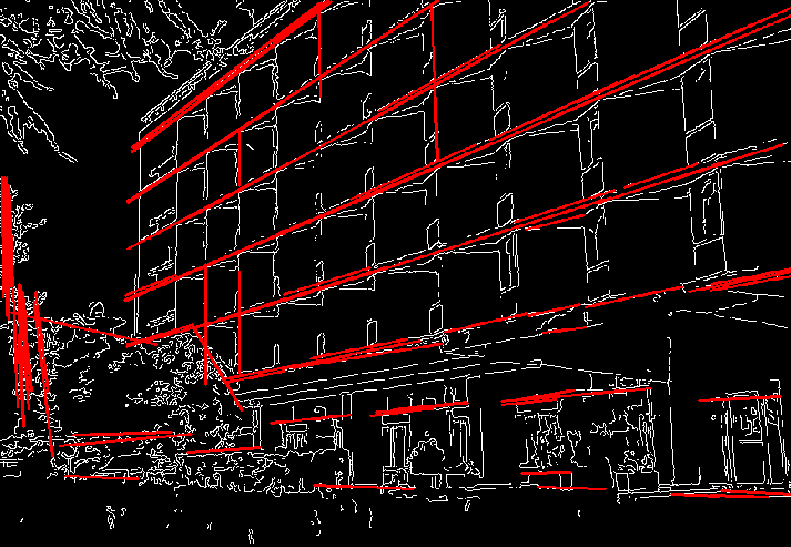
\includegraphics[width=67mm, keepaspectratio]{figures/houghline_building_2.png}
\caption{Egyenesek keresése Hough-transzformáció használatával.\\Forrás: \url{http://href.hu/x/c91h}}
\label{fig:houghlines}
\end{figure}

A \textbf{Hough-transzformáció} erre a problémára kínál megoldást. Feladata egyszerű formák, úgymint egyenesek, körök, ellipszisek keresése képeken. Az alakzatok keresését a transzformáció egy ún. paramétertérben végzi egy szavazási mechanizmus segítségével. A felismert potenciális objektumok az akkumulátortér -- a paramétertér egyfajta futás közbeni leképezése -- lokális maximumai alapján adódnak.

\bigskip

Történelmi áttekintésként megjegyezhetjük, hogy a Hough-transzformációt Paul~Hough alkotta meg 1959-ben buborékkamra-fényképek gépi analíziséhez \cite{hough_eredeti}. Ebben a cikkben Hough még csak egyenesek felismeréséről beszél. A manapság használt transzformációt Richard~Duda és Peter~Hart fejlesztette ki 1972-ben ,,általánosított Hough-transzformáció'' néven \cite{hough_duda}, tíz évvel azután, hogy Paul Hough szabadalmaztatta módszerét. Az õ kiegészítésük már lehetõvé tette, hogy a transzformáció nemcsak egyenesek, hanem körök és más analitikusan leírható görbék keresésére is felhasználható legyen.

A gépi látás felhasználói körében azonban igazán csak Dana~H.~Ballard 1981-es cikke \cite{hough_ballard} nyomán lett népszerű, aki a transzformáció még további felhasználási lehetőségeit vetette fel. Eredményeinek köszönhetően a módszer analitikusan nem (vagy csak nehezen) leírható formák keresésére is alkalmazhatóvá vált. Félreértésekre adhat okot, hogy mind Duda és Hart, mind Ballard az ,,általánosított'' megnevezést használja a módszer általuk kitalált kiegészítéseinek. A továbbiakban az ,,általános'' jelzőt a Duda--Hart-féle kiegészítés megnevezésére használom, ahol Ballard módszeréről esik szó, azt külön jelzem.

\bigskip

A transzformáció általános formájában tehát analitikusan leírható formák keresésére használható. A legegyszerűbb ilyen forma az egyenes, ennek segítségével érthető meg legkönnyebben az algoritmus működési elve. A \sectref{egyenesek_keresese} szakaszban ezért az egyenesek, majd a \sectref{korkereses} szakaszban a körök keresésének elméletére térek ki.

%............................................................................
\subsection{Egyenesek keresése}\label{sect:egyenesek_keresese}
%............................................................................

%. . . . . . . . . . . . . . . . . . . . . . . . . . . . . . . . . . . . . .
\subsubsection{Egyenes-reprezentációk}\label{sect:egyenes_reprezentaciok}
%. . . . . . . . . . . . . . . . . . . . . . . . . . . . . . . . . . . . . .

Egyenesek leírására többféle modell használható. Az egyenes ,,klasszikus'' modellje Descartes-koordinátarendszerben az

\begin{align}\label{eq:egyenes_klasszikus}
y = m \cdot x + b
\end{align}

reprezentáció, ahol $ m $ az egyenes meredeksége (iránytangense), a $ b $ konstans az ordinátatengely-metszet, vagyis az egyenes és az $ y $ tengely metszéspontja.

A \eqref{egyenes_klasszikus} egyenlettel megadott modellel az a probléma, hogy a koordinátarendszer $ y $ tengelyével párhuzamos, vagy ahhoz közelítő egyenesek leírására nem használható $ m $ végtelen nagy értéke miatt. Nem szerencsés azonban az ilyen ,,függőleges'' egyenesek kizárása a számításból. Ennek kiküszöbölésére -- jelen esetben -- jobb modellként segítségül hívhatjuk a \textbf{Hesse-féle normálalakos} reprezentációt. Ez az

\begin{align}\label{eq:egyenes_hesse}
r = x \cdot \cos \theta + y \cdot \sin \theta
\end{align}

egyenlettel adja meg a kívánt egyenest, ahol $ r $ az origótól mért távolságot, $ \theta $ pedig az egyenes pozitív valós féltengellyel bezárt szögét jelenti (lásd \figref{repr_line} ábra). Ezzel a megvalósítással már nem ütközik akadályba az $ y $ tengelyhez közelítő egyenesek modellezése.

\begin{figure}[!ht]
\centering
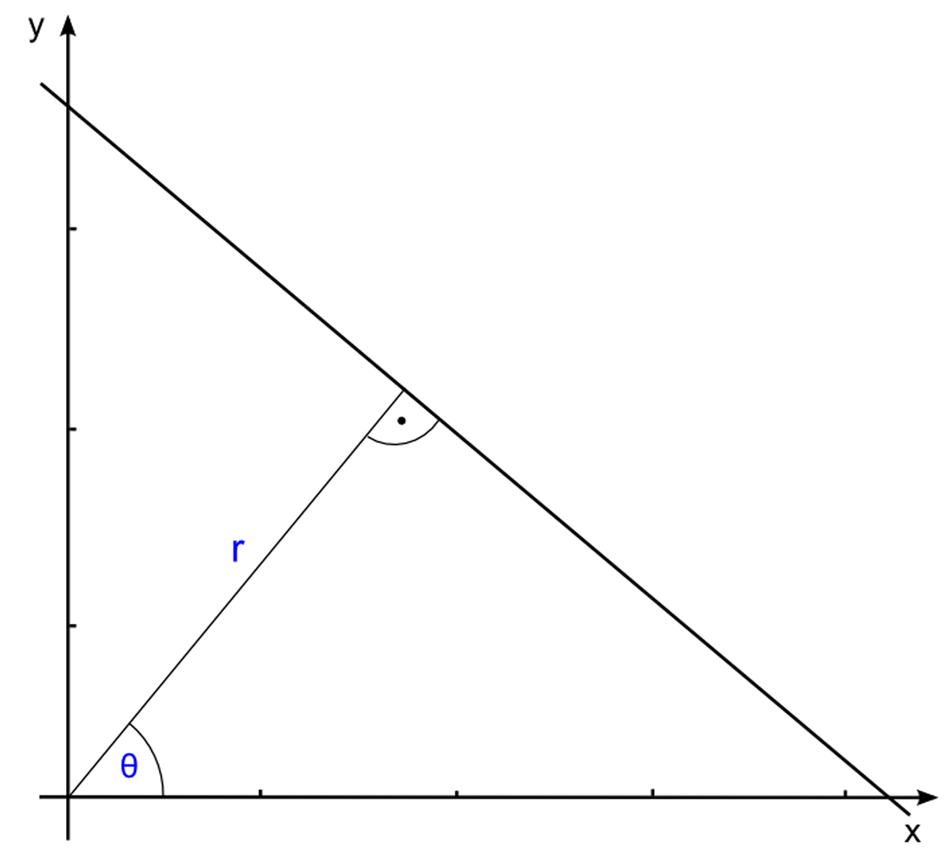
\includegraphics[width=80mm, keepaspectratio]{figures/repr_line.png}
\caption{Egyenes jellemzése $ r $ és $ \theta $ paraméterekkel.}
\label{fig:repr_line}
\end{figure}

\bigskip

Érdekességként megemlíthető, hogy bár nyilvánvalónak látszik a Hesse-féle normálalak előnyösebb volta, Paul Hough eredeti szabadalmában\footnote{U.S. Patent 3,069,654 -- \url{http://www.google.com/patents?q=3069654}} mégis az $ y = m \cdot x + b $ formát használta az egyenesek jellemzésére. Az $ (r, \theta) $ paraméterezés Duda és Hart már hivatkozott cikke nyomán vált általánosan használttá. \cite{hough_duda}

%. . . . . . . . . . . . . . . . . . . . . . . . . . . . . . . . . . . . . .
\subsubsection{A paramétertér és az akkumulátor}\label{sect:parameterter_akkumulator}
%. . . . . . . . . . . . . . . . . . . . . . . . . . . . . . . . . . . . . .

Minden képtérbeli egyenes tehát \eqref{egyenes_hesse} felhasználásával megfeleltethető a paramétertérben egy $ (r, \theta) $ párral jellemzett pontnak. Az egyértelmű megfeleltetés végett két lehetőségünk is adódik a paraméterek korlátainak megválasztására. Ezek formálisan

\begin{align}\label{eq:param180}
\theta \in \left[ 0,180^{\circ} \right) \quad \wedge \quad r \in \mathbf{R}
\end{align}

vagy

\begin{align}\label{eq:param360}
\theta \in \left[ 0,360^{\circ} \right) \quad \wedge \quad r \geq 0
\end{align}

Az $ (r, \theta) $ párok terét \textbf{paramétertérnek}, vagy \textbf{Hough-térnek} hívjuk. A paramétertér dimenzióját az ismeretlen paraméterek száma adja, egyenesek esetében ez tehát kettő.

Egy $ (x,y) $ ponton keresztül végtelen sok egyenes húzható, és minden egyenes kielégíti a \eqref{egyenes_hesse} összefüggést. Ezek az egyenesek a paramétertérben ábrázolva egy szinusz-jellegű görbét alkotnak. Természetesen nem határozhatunk meg tetszőleges pontossággal egy pontot, és nem is vehetünk számításba minden (végtelen számú) olyan egyenest, ami az adott ponton átmegy. Szükség van ezért a paramétertér diszkretizálására.

\bigskip

A paramétertér gyakorlati (kvantált) reprezentációja az \textbf{akkumulátor}. Az akkumulátor egy tömb, dimenziószáma megegyezik a paramétertér dimenziószámával.

A tömbök indexelése egész számokkal történik ezért az $ r $ paramétert egész számokra célszerű kvantálnunk. A $ \theta $ paraméter kvantálásához pedig a végtelen sok egyenes figyelembe vétele helyett az $ (x,y) $ koordinátán keresztül húzhatunk egyeneseket $ \varDelta \theta $ fokonként. Ebből következően a \eqref{param180} vagy \eqref{param360} összefüggések alapján az akkumulátor ezen dimenzióját $ 180^{\circ} / \varDelta \theta $, illetve $ 360^{\circ} / \varDelta \theta $ darab diszkrét részre osztja. A $ \varDelta \theta $ paraméter megválasztásával, a módszer ,,finomságát'' növelhetjük. Például $ \varDelta \theta = 5^{\circ} $ választás esetén a transzformáció csak a pozitív valós féltengellyel $ 0, 5, 10, ... $ fokot bezáró egyenesek felismerésére képes. Túl kis érték választása esetén viszont az eljárás memória- és időigénye fog az egekbe szökni. A $ \varDelta \theta $ érték gondos megválasztásával tehát a pontosság és gyorsaság egy lehetőleg optimális értékét kell meghatároznunk.

Gyakorlati szabályként elmondható, hogy 1 fok pontosságnál többre ritkán van szükség. Túl vastag vonalak (amik pedig logikailag összefüggő egyenesek), zajos kép, vagy túl rövid vonalszakaszok esetén így is romlik a felismerés esélye. Hogy miért, arra a következő szakasz -- a szavazási mechanizmus ismertetése -- ad választ.

%. . . . . . . . . . . . . . . . . . . . . . . . . . . . . . . . . . . . . .
\subsubsection{A keresés folyamata}\label{sect:kereses_folyamata}
%. . . . . . . . . . . . . . . . . . . . . . . . . . . . . . . . . . . . . .

A továbbiakban tételezzük fel, hogy a kép bináris, és megfelelően előfeldolgozott (pl. élkeresés, küszöbözés), azon már csak a felismerni kívánt egyenesek pontjai találhatóak. A háttér képpontjait jelölje a 0 érték, az érdekes pontokat tartalmazó előtér képpontjai legyenek 1 értékűek.

A keresés folyamán bejárjuk a képteret pixelrõl pixelre. A 0 értékű képpontok biztosan nem részei egy képen található egyenesnek sem, ezért ezekkel nem kell foglalkozunk. Ha 1 értékű pixelt találunk az $ (x,y) $ helyen, az potenciálisan része lehet egy, a képen található egyenesnek. Az akkumulátor minden $ \theta $ értékhez (pl. fokonként) meghatározzuk az $ (x,y) $ ponton átmenő, $ \theta $ irányú egyenes origótól vett $ r $ távolságát a \eqref{egyenes_hesse} összefüggés alapján. Az akkumulátortömb értékét minden így kiszámolt $ (r,\theta) $ indexekkel jelölt helyen megnöveljük ($ r $ meghatározásánál természetesen a tömb kvantáltságát figyelembe véve). Ezt a folyamatot úgy is mondhatjuk, hogy az $ (x,y) $ pont a kiszámított $ (r, \theta) $ pontok halmazára, vagyis ezen paraméterek által a képtérben képviselt egyenesekre \textbf{,,szavaz''}.

Az algoritmus első fázisának lefutása után az akkumulátortömböt kell vizsgálnunk. Optimális esetben a képen egy egyenesre eső pixelek mindegyike (a többi más szavazatuk mellett) szavazott a ,,valódi'' egyenest jelentő $ (r, \theta) $ párra. Az akkumulátortömb maximális értékű $ (r, \theta) $ elemei adják meg tehát a képen található egyeneseket. A zaj, az esetleg több pixel széles vonalak, és a kvantálási pontatlanság miatt azonban célravezetőbb \textbf{lokális maximumokat} (lásd \figref{houghparam} ábra) keresni az akkumulátortömbben így meghatározva a \textbf{legvalószínűbb} egyenesek $ r $ és $ \theta $ paramétereit.

\begin{figure}[!ht]
\centering

\includegraphics[width=67mm, keepaspectratio]{figures/houghparam_1.png}\hspace{1cm}

\includegraphics[width=67mm, keepaspectratio]{figures/houghparam_2.png}
\caption{A képtér (balra) és az ebből származó paramétertér (jobbra) egyenesek keresése során.\\Forrás: \url{http://href.hu/x/c91i}}
\label{fig:houghparam}
\end{figure}

Az elõzõ szakasz végén felvetett problémát most már megválaszolhatjuk. A túl nagy zaj miatt megnő azon képpontok száma, amik nem részei egy egyenesnek sem. Azonban szavazni ezek a képpontok is szavaznak, ezzel mintegy ,,háttérzajt'' adva az akkumulátortömbnek. Túl vastag vonalak esetén pedig több, látszólag helyes paraméterezésű egyenes adódna ugyanarra a vonalra (pl. egymással a vonalon belül párhuzamos egyenesek, de kellően vastag vonal esetén akár ,,átlós'' egyenesek is). Az első esetben az akkumulátortömb elemeinek átlagos értéke nő meg, a második esetben pedig a sok egymáshoz közeli szavazat miatt lokális maximumok értékei kerülnek közelebb az átlagos tömbértékekhez. Mindkét esetben nehezebbé válik a lokális maximumok pontos meghatározása, ez pedig drasztikusan csökkentheti a keresés pontosságát.

%............................................................................
\subsection{Körkeresés}\label{sect:korkereses}
%............................................................................

%. . . . . . . . . . . . . . . . . . . . . . . . . . . . . . . . . . . . . .
\subsubsection{Körök reprezentációja}\label{sect:korok_reprezentacioja}
%. . . . . . . . . . . . . . . . . . . . . . . . . . . . . . . . . . . . . .

A körökhöz megfelelő reprezentáció megtalálásához még annyit sem kell törnünk a fejünket, mint az egyeneseknél tettük. Descartes-koordinátarendszerben az $ (x_{0}, y_{0}) $ középpontú $ r $ sugarú körvonal pontjait az

\begin{align}\label{eq:kor_koogeom}
( x - x_{0})^{2} + (y - y_{0})^2 = r^2
\end{align}

egyenlet adja meg (\figref{repr_circle} ábra). Szögfüggvények használatával az \eqref{kor_koogeom} egyenletet átalakíthatjuk

\begin{align}\label{eq:kor_param}
x &= x_{0} + r \cdot \cos \theta \nonumber \\
y &= y_{0} + r \cdot \sin \theta
\end{align}

formára, ahol $ (x_{0}, y_{0}) $ szintén a kör középpontjának koordinátái, $ r $ a sugár, $ \theta $ pedig a körvonal egy pontját a kör középpontjával összekötő szakasz pozitív valós féltengellyel bezárt szögét jelenti.

\begin{figure}[!ht]
\centering
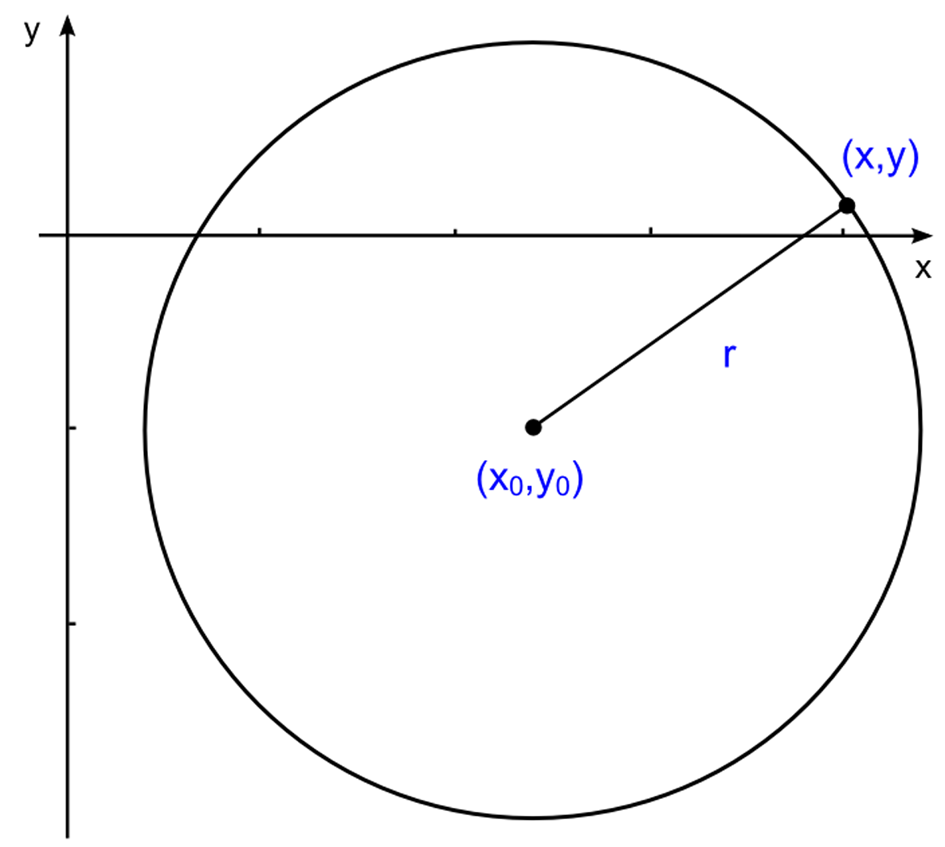
\includegraphics[width=80mm, keepaspectratio]{figures/repr_circle.png}
\caption{Körök reprezentációja.}
\label{fig:repr_circle}
\end{figure}

%. . . . . . . . . . . . . . . . . . . . . . . . . . . . . . . . . . . . . .
\subsubsection{A paramétertér körök esetében}\label{sect:korok_parameterter}
%. . . . . . . . . . . . . . . . . . . . . . . . . . . . . . . . . . . . . .

Látható, hogy körök esetében már csak akkor elegendő két paraméter -- az $ (x_{0}, y_{0}) $ középpont-koordináták -- a forma leírásához, ha előre adott sugarú köröket keresünk, vagyis $ r $ konstans. Ez azonban csak bizonyos esetekben használható, általános esetben túl nagy megkötést jelent. Tehát a paramétertér dimenziószámát növelnünk kell: az $ r $ sugárparaméter dimenziójával együtt az már \textbf{három dimenziós lesz}.

A paraméterteret az akkumulátor tömb mivoltából adódóan itt is egész számokra kell kvantálnunk. Körkeresés esetén az akkumulátor tehát egy három dimenziós tömb, amely a középpont két koordinátájának és a sugárnak egész értékeivel indexelhető. Már a pontos algoritmus ismerete nélkül is látszik, hogy a potenciális körök keresése jóval komplexebb művelet az ismeretlen paraméterek magasabb száma miatt.

%. . . . . . . . . . . . . . . . . . . . . . . . . . . . . . . . . . . . . .
\subsubsection{A körkeresés folyamata}\label{sect:korok_keresese}
%. . . . . . . . . . . . . . . . . . . . . . . . . . . . . . . . . . . . . .

Az alaphelyzet legyen az egyenesek keresésekor felállított: a felismerni kívánt körvonalak képpontjai legyenek 1, a háttér felismerés szempontjából érdektelen képpontjai pedig legyenek 0 értékűek.

A bejárás során 1 értékű pixelt találva jóval több számítani valónk van, mint egyenesek esetében. Az akkumulátor \textbf{összes lehetséges $ r $ sugárparaméterére} meg kell határoznunk a potenciális körök középpontjait. Ehhez felhasználjuk az \eqref{kor_param} összefüggéseket $ r $ és $ \theta $ ismeretében ($ \theta $ lehetséges értékeinek megválasztása -- tipikusan például fokonként -- azonos elven történhet a \sectref{parameterter_akkumulator} szakaszban olvashatóakkal).

Hogy próbálhatjuk meg csökkenteni a rengeteg számítást? Egyfelől \textbf{korlátozhatjuk} $ r $ lehetséges értékeinek halmazát. Az értékeknek $ r_{min} $ alsó és $ r_{max} $ felsõ korlátot adva a keresést a két érték közötti sugarú körökre szűkíthetjük. Némi előzetes információ birtokában (körülbelül, vagy a kép oldalainak arányában mekkora köröket kell keresnünk) jelentősen csökkenthető a számítási idő- és tárigény.

Másfelől pedig felhasználhatunk lokális információkat is: a vizsgálat alatt lévő képpont egy adott ablaknyi környezetét vizsgálva, meghatározhatjuk a körvonal adott pontbeli \textbf{gradiensét}. Ez az információ felhasználható a középpont keresésében, ugyanis a kör középpontjának a körvonalpont normálisán kell feküdnie. Így, ha nem is egyetlen kitüntetett irányra, de a számítási pontatlanságot és a zajt figyelembe véve egy szűk tartományra korlátozhatjuk a keresett körközéppontok irányát. Ez a választott tartomány méretével fordított arányosságban csökkenti a szükséges számítások számát. Példának okáért, ha a kiszámított gradiens segítségével akár csak 90 fok pontossággal meg tudjuk határozni a pontban vett normális irányát, a számítások háromnegyedét nem kell elvégeznünk, ráadásul az akkumulátortömb sem telítődik feleslegesen olyan paraméterekkel, amelyekből biztosan (vagy elég nagy valószínűséggel) nem fog helyes megoldás születni.

%. . . . . . . . . . . . . . . . . . . . . . . . . . . . . . . . . . . . . .
\subsubsection{Egyéb körkeresési eljárások}\label{sect:korok_kiegeszites}
%. . . . . . . . . . . . . . . . . . . . . . . . . . . . . . . . . . . . . .

A körkeresésre használt Hough-transzformáció további kiegészítéseivel találkozhatunk H. K. Yuen \textit{et al} hivatkozott cikkében \cite{hough_circles}. A cikkben az előző alfejezetben ismertetett sztenderd változat mellett még további négy módosulat vizsgálatát és ezek összehasonlítását végzik el a szerzők. Ezek közül a cikkben ,,2-1 Hough-transzformációnak'' néven hivatkozott módszert emelném ki, a későbbiek során ugyanis ennek fontos szerepe lesz. Elnevezésként a cikkben használt ,,21HT'' rövidítést fogom használni.

A \textbf{21HT} módszer a \cite{hough_21_davies} és \cite{hough_21_illingworth} számon hivatkozott cikkekben volt először használatos. A kiegészítés felhasználja a rendelkezésre álló gradiens-információt (lásd: \sectref{korok_keresese}), és ennek ismeretében pedig a problémát két részre osztja. Mivel a kör középpontjának a körvonalpontok normálisán kell feküdnie, ezen normálisok közös metszéspontja valójában tehát meghatározza a középpontot. Egy kétdimenziós akkumulátortömb pedig elég minden pont saját normálisára esõ szavazatainak nyilvántartásához. Ezután a sugár meghatározása a következő módszerrel történhet: meghatározzuk minden pont és az előző lépésben kiszámított középpont-jelölt távolságát, majd ezekből az információkból egy sugár-hisztogramot állítunk elő. Ennek vizsgálatával már meghatározhatjuk a középpontokhoz tartozó sugarakat is. A módszer tárigénye az eredeti megközelítéshez képest jóval kisebb, hiszen csak egy \textbf{2D akkumulátort} és egy \textbf{1D hisztogramot} kell használnunk -- innen a módszer ,,2-1'' elnevezése.

Eredmények tekintetében az összehasonlító cikk szerint a 21HT módszer felveszi a versenyt a sztenderd megoldással. Igaz, hogy a kétfázisú számítás miatt az első fázisban összeszedett hiba szükségszerűen rárakódik a második fázisra, ezt a pontatlanságot ellensúlyozni tudja a módszer jelentősen kisebb tárigénye.

%............................................................................
\subsection{Kiegészítések}\label{sect:kiegeszitesek}
%............................................................................

A meglévõ módszer továbbfejlesztésekor két irányba is elindulhatunk:

\begin{enumerate}
 \item egyrészt növelhetjük az algoritmus teljesítőképességét,
 \item másrészt bővíthetjük a felismerhető formák halmazát.
\end{enumerate}

Ebben a szakaszban mindkét lehetséges fejlesztési irány eredményeiről szeretnék röviden beszámolni a témában fellelhető szakirodalom felhasználásával.

\bigskip

Az elsõ irányba mutató fejlesztések közül néhánnyal már találkozhattunk jelen dolgozat keretein belül is. Az \sectref{korok_keresese} alszakaszban előkerült a gradiensinformáció felhasználása és az elõzetes tudás alapján történő megfelelő korlátok bevezetése a számítás gyorsítása végett. Ebben a témában mindenképp megemlítendõ még a kernel alapú Hough-transzformáció.

A \textbf{kernel alapú megvalósítás} lehetőségét a szerzők -- Fernandes és Oliveira -- 2008-as cikkükben \cite{hough_fernandes} vetették fel, tehát a módszer meglehetősen friss. Állításuk szerint valósidejű működés érhető el viszonylag nagy képek esetén is a szavazási protokoll továbbfejlesztésének köszönhetően. A módszer egyeneskereséskor az $ (r, \theta) $ paraméterezésen nem változtat, de nem önmagukban álló pontokat, hanem körülbelül egy irányban álló pixelek klasztereit (csoportjait) veszi figyelembe. Minden klaszterben egy megfelelő irányba forgatott elliptikus Gauss-kernellel végzett konvolúció hivatott a csoportra vonatkozó bizonytalanságot modellezni. Ez a megközelítés nemcsak hogy a szavazatok számának csökkentésével képes az algoritmus sebességét növelni, hanem a protokollnak köszönhetően sokkal tisztább akkumulátort is eredményez. A háttérzajtól mentes tömbben pedig jóval könnyebben tudjuk a lokális maximumokat detektálni. Ezzel összességében az eddigieknél gyorsabb és pontosabb egyenesdetektálást tudunk kivitelezni.

\bigskip

Felismerhetõ formák tekintetében a módszer bővíthető az általános analitikus 2D görbék mellett 3D képeken testek felismerésére. Ezen kívül semmiképp nem hagyhatjuk szó nélkül a Ballard-féle általánosított Hough-transzformációt sem.

Három dimenzióban a \textbf{testek felismerése} a két dimenziós esetekhez hasonlóan történik -- hasonló buktatókkal és legtöbbször további járulékos memória- és számításigénnyel. Síkoknál például az egyenesekhez hasonlóan a megszokott reprezentáció nem használható függőleges síkok keresésére. A megoldást ebben az esetben a gömbi koordinátarendszerre való átállás jelenti, ahol a sík már normálvektorával és az origótól való távolságával jellemezhető (a paramétertér tehát három dimenziósra adódik). Gömbök, hengerek, ellipszoidok keresése szintén a két dimenziós esetek tapasztalatainak felhasználásával történhet. Az új, akár térbeli formák keresése kombinálható az eddig megismert teljesítménynövelő eljárásokkal: a már megismer eljárások használhatók a keresés során, természetesen adott esetben három dimenzióra vonatkoztatva azokat.

Dana H. Ballard általánosított transzformációja \cite{hough_ballard} -- amint az már jelen dolgozat keretein belül is előkerült -- lehetővé teszi modelljükkel reprezentált általános objektumok felismerését a \textbf{mintafelismerés} alapelvét kihasználva. A modell előfordulásainak keresése a képtérben -- ahogy Ballard megmutatta -- szintén megoldható paraméterek akkumulálásával. Válasszuk ezen paramétereknek a modellt a képtérbe átvivő transzformáció (vagy transzformációk) paramétereit! Például ha csak a modell pozícióját keressük, akkor mindössze eltolási paramétereket kell figyelembe vennünk, ezek akkumulálásával a megszokott módon és eredményességgel ismerhetjük fel az adott objektum helyzetét. Azonban a módszer a transzláció (eltolás) invariancia mellett rotáció (forgatás) és skálázás (méret) invariánssá is tehető, igaz a paramétertér dimenziószámának növelése árán. Láthatjuk, hogy a mintafelismerés és a szavazási mechanizmus előnyeinek ötvözésével ez az eljárás igazán komoly fegyver lehet a képfeldolgozási eszköztárunkban.

\begin{figure}[!ht]
\centering
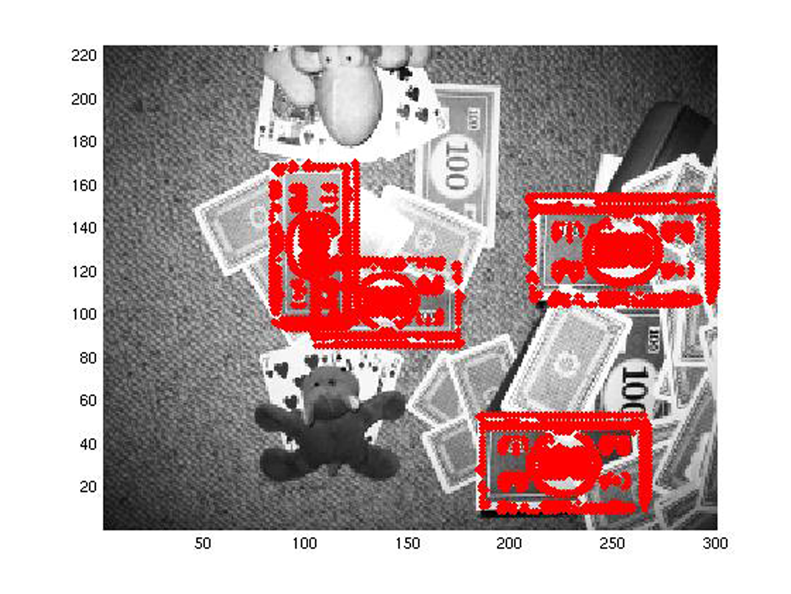
\includegraphics[width=67mm, keepaspectratio]{figures/generalhough_money_1.png}\hspace{1cm}
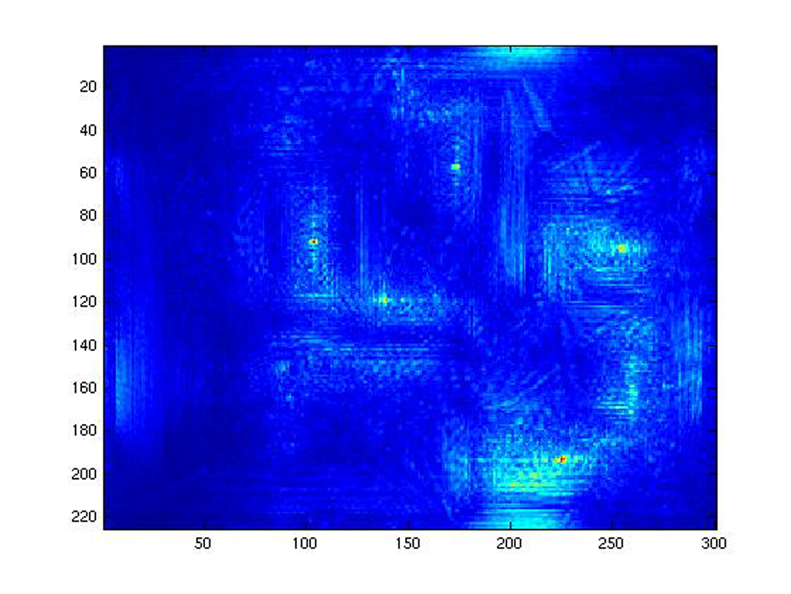
\includegraphics[width=67mm, keepaspectratio]{figures/generalhough_money_2.png}
\caption{Kép- és paramétertér az általánosított Hough-transzformáció használata közben.\\Forrás: \url{http://href.hu/x/c91m}}
\label{fig:generalhough}
\end{figure}

%............................................................................
\subsection{Összegzés}\label{sect:hough_osszefoglalas}
%............................................................................

Az eddigiek alapján látszik, hogy a transzformáció felhasználhatóságának szűk keresztmetszetét leginkább a nagy számításigénye adja. Ez egyben legfőbb \textbf{hátránya} is: a számításigény a paramétertér dimenziószámának, vagy a kép méretének növekedésével egyre csak növekszik. A dimenziók száma tehát korlátot ad a transzformáció gyakorlati felhasználhatóságának, ezért eredeti formájában leginkább csak egyenesek, vagy körök keresésére használják. A körök keresésének lehetősége azonban kielégítheti a pupillakövetési probléma által támasztott követelményeket. A követés során \textbf{előnyére} válhat, hogy a szavazási mechanizmus használata miatt meglehetősen zajos képeken is képes lehet a pupillakontúr megbízható felismerésére. Valós életből vett tesztesetekben -- pupillakövetés esetén ezek számítanak -- pedig ez korántsem elhanyagolható szempont.


\newpage
%,,,,,,,,,,,,,,,,,,,,,,,,,,,,,,,,,,,,,,,,,,,,,,,,,,,,,,,,,,,,,,,,,,,,,,,,,,,,
\section{Objektumdetektálás és -követés}\label{sect:objdetect}
%,,,,,,,,,,,,,,,,,,,,,,,,,,,,,,,,,,,,,,,,,,,,,,,,,,,,,,,,,,,,,,,,,,,,,,,,,,,,

Az objektumdetektálás többnyire magasabb absztrakciós szintű képi elemek megtalálására törekszik. Minél magasabb szintű a detektálni kívánt jellemző, azzal arányosan nő a megtalálásához szükséges számítási igény is -- hiszen a kép egyre mélyebb megértésére van szükség. Ezáltal veszélybe kerülhet a valós idejű feldolgozási sebesség. A megnövekedett számítási igény azzal kompenzálható, hogy az objektumdetektálást nem minden képkockán végezzük el, hanem két detektálási lépés között próbáljuk egy ,,olcsóbb'' algoritmus használatával követni a felismert objektumot.

A fent vázolt felépítésre lehet jó példa a Viola--Jones objektumdetektor és a Lucas--Kanade optikai áramlás együttes használata, ezek elméleti alapjait mutatom be a szakasz további részében.

%............................................................................
\subsection{A Viola--Jones objektumdetektor}\label{sect:viola}
%............................................................................

A Paul Viola és Michael Jones által 2001-ben elővezetett \cite{vj} Viola--Jones objektumdetektor az első olyan objektumfelismerő rendszer, megközelítheti, vagy akár teljesítheti is a valósidejű feldolgozás által támasztott követelményeket. A rendszer eleinte arcdetektálás céljából készült, de mint kiderült, működése könnyen általánosítható, így megfelelő tanítás után bármilyen objektum felismerésére képes lehet.

\begin{figure}[!ht]
\centering
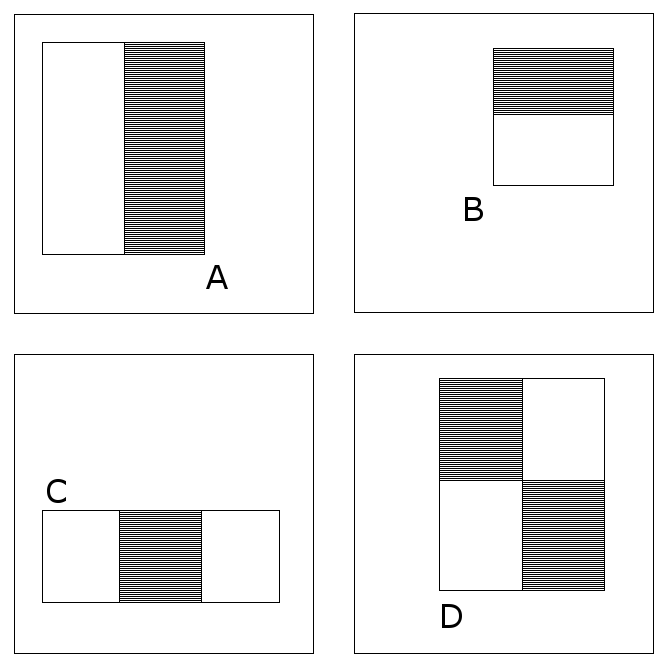
\includegraphics[width=50mm, keepaspectratio]{figures/features.png}
\caption{A Viola és Jones által használt jellemzőtípusok.\\Forrás: \cite{vj}}
\label{fig:features}
\end{figure}

Az osztályozó úgynevezett \emph{jellemzőkkel} (features) dolgozik, amelyek téglalap alakú területeket alapul véve a bennük lévő képpontok összegét jelentik. Ebben a formában a jellemzők rokonságot mutatnak a Haar bázisfüggvényekkel, amelyek az objektumdetektálásban korábban meghatározó \emph{wavelet transzformációnál} használatosak. Lehetséges jellemzőtípusokat mutat be a \figref{features} ábra.

A jellemző-alapú, úgynevezett \emph{integrális} képreprezentáció esetén az egyes jellemzők ugyan nagyon egyszerűek, viszont konstans időben kiértékelhetők. A jellemzők gyors értékelhetősége azonban nem kompenzálja nagy számukat. Minden egyes területre minden jellemzőt kiértékelve csökkenne a rendszer használatával nyert előny. Ennek kiküszöbölésére a betanítási fázisban a Viola--Jones detektor az AdaBoost \cite{freund} eljárás egy módosított változatát alkalmazza, amely segít kiválasztani a leginkább fontos jellemzőket, valamint korlátokat ad a kész osztályozó általánosító képességére.

Ha csak az AdaBoost eljárás által kiválasztott fontos jellemzőket értékeljük ki, a rendszer alapesetben akkor sem képes a valós idejű osztályozásra. Ennek kivédésére a tanítási folyamatban az egyes elemi osztályozókat egymás után kötik (kaszkádosítják), és minden osztályozó bemenetére csak azok a minták jutnak, amelyeket a sorban előtte lévő összes osztályozó elfogadott.

%............................................................................
\subsection{A Lucas--Kanade optikai áramlás eljárás}\label{sect:optflow}
%............................................................................

A számítógépes látás területén az optikai áramlás közelítésének kérdése fontos kutatási terület, ennek megfelelően a problémára számos különböző megoldás született. A Bruce D. Lucas és Takeo Kanade által 1981-ben nyilvánosságra hozott \cite{lk} differenciális algoritmus manapság az egyik legszélesebb körben használt módszer optikai áramlás számításakor.

\begin{figure}[!ht]
\centering
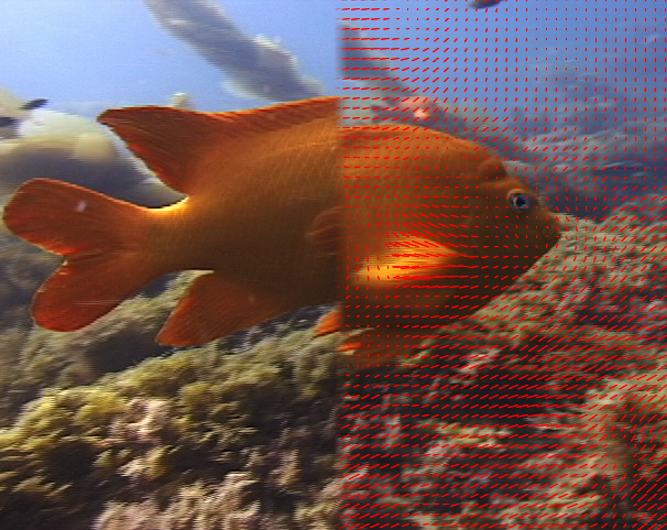
\includegraphics[width=80mm, keepaspectratio]{figures/opticalflow.png}
\caption{A kép jobb oldalán piros nyilak jelképezik az optikai áramlást.\\Forrás: \url{http://href.hu/x/dz36}}
\label{fig:optical_flow}
\end{figure}

Az eljárás feltételezi, hogy az áramlás konstans a vizsgált képpont helyi környezetében, és ebben a környezetben (ablakban) a legkisebb négyzetek módszerével próbálja kiszámolni az aktuális pont elmozdulásvektorát. Azzal, hogy nem egy-egy képpontot, hanem egy kis lokális ablakot vesz figyelembe a számítás során, a Lucas--Kanade eljárás kevésbé érzékenyen reagál a zajos képekre. Másrészt viszont a lokális tulajdonság hatására az eljárás nem tud információt szolgáltatni a kép nagy, összefüggő, azonos intenzitású területein.

%. . . . . . . . . . . . . . . . . . . . . . . . . . . . . . . . . . . . . .
\subsubsection{Matematikai háttér}\label{sect:matrixok}
%. . . . . . . . . . . . . . . . . . . . . . . . . . . . . . . . . . . . . .

Tegyük fel, hogy két egymás követő időpillanatban a képek közti eltérés megfelelően kicsi. Az optikai áramlás eljárás alapegyenlete ebben az esetben következő

\begin{align}\label{eq:optflow_alap}
I_x V_x + I_y V_y = - I_t
\end{align}

formában írható fel, ahol $V_x$ és $V_y$ az $(x,y,t)$ képpont sebességének (vagyis optikai áramlásának) $x$ és $y$ koordinátái, $I_x$, $I_y$ és $I_t$ pedig a kép parciális deriváltjai.

A Lucas--Kanade eljárásban egy, a vizsgált képpont körüli ablak tartalmát vesszük figyelembe, és feltesszük, hogy az áramlás ezen a régión belül állandó. A \eqref{optflow_alap} egyenletet ennek megfelelően a következő formára hozhatjuk

\begin{align}\label{eq:optflow_lk}
I_x(q_1)V_x + I_y(q_1)V_y &= - I_t(q_1) \nonumber \\
I_x(q_2)V_x + I_y(q_2)V_y &= - I_t(q_2) \nonumber \\
&\vdots \nonumber \\
I_x(q_n)V_x + I_y(q_n)V_y &= - I_t(q_n)
\end{align}

amelyben $q_1$, $q_2$, $\ldots$, $q_n$ az aktuálisan vizsgált pont körüli ablak egyes képpontjai.

A \eqref{optflow_lk} egyenletet $Av = b$ formában, mátrixokkal is felírhatjuk, ekkor 

\begin{align}\label{eq:optflow_matrix}
A &= \left[ \begin{array}{cc} I_x(q_1) & I_y(q_1) \\ I_x(q_2) & I_y(q_2) \\ \vdots & \vdots \\ I_x(q_n) & I_y(q_n) \end{array} \right] \nonumber \\
v &= \left[ \begin{array}{c} V_x \\ V_y \end{array} \right] \nonumber \\
b &= \left[ \begin{array}{c} -I_t(q_1) \\ -I_t(q_2) \\ \vdots \\ -I_t(q_n) \end{array} \right]
\end{align}

A \eqref{optflow_matrix}-ban definiált egyenletrendszer felülhatározott, vagyis több egyenlet szerepel benne, mint ismeretlen. A Lucas--Kanade algoritmus a legkisebb négyzetek módszerével számítja ki a sebességkomponenseket, vagyis

\begin{align}\label{eq:optflow_seb1}
v &= \frac{A^T b}{A^T A}
\end{align}

ami \eqref{optflow_matrix}-at behelyettesítve a következő alakra hozható

\begin{align}\label{eq:optflow_seb2}
\left[ \begin{array}{c} V_x \\ V_y \end{array} \right] &= \left[ \begin{array}{cc} \sum_{i=1}^n I_x(q_i)^2 & \sum_{i=1}^n I_x(q_i)I_y(q_i) \\ \sum_{i=1}^n I_x(q_i)I_y(q_i) & \sum_{i=1}^n I_y(q_i)^2 \end{array} \right]^{-1} \left[ \begin{array}{c} - \sum_{i=1}^n I_x(q_i)I_t(q_i) \\ - \sum_{i=1}^n I_y(q_i)I_t(q_i) \end{array} \right]
\end{align}

vagyis az aktuálisan vizsgált $q_1$, $q_2$, $\ldots$, $q_n$ pontokat tartalmazó ablak $p$ középpontjának $x$ és $y$ irányban vett sebességkomponenseit adja meg közvetlenül a \eqref{optflow_seb2} egyenlet.

%............................................................................
\subsection{Összegzés}\label{sect:detect_osszefoglalas}
%............................................................................

A \sectref{viola} szakaszban felsorolt eljárásoknak köszönhetően a Viola--Jones objektumdetektor képes az elődeinél jóval gyorsabban osztályozni a bemenetére küldött képeket. Ha azonban nem is lehetséges a videofolyam minden egyes képkockáján a rendelkezésre álló időn belül önállóan döntést hozni, valamilyen kiegészítő technika használatával (pl. a felismert objektumok optikai áramlás-alapú követése) \emph{valós idejű} objektumdetektáló rendszer létrehozása válik lehetővé.

A Lucas--Kanade optikai áramlás-alapú követés jó kiegészítésként szolgálhat egy nagyobb számításigényű objektumdetektor mellé. Azonban a használat során a két módszer egymáshoz viszonyított ideális összetételének megtalálása döntő a követés pontossága és gyorsasága szempontjából. 




\newpage
%,,,,,,,,,,,,,,,,,,,,,,,,,,,,,,,,,,,,,,,,,,,,,,,,,,,,,,,,,,,,,,,,,,,,,,,,,,,,
\section{Blob-műveletek}\label{sect:blob}
%,,,,,,,,,,,,,,,,,,,,,,,,,,,,,,,,,,,,,,,,,,,,,,,,,,,,,,,,,,,,,,,,,,,,,,,,,,,,

A képfeldolgozásban a \emph{blob} fogalmat a szó ,,folt'' értelmében használják, nem keverendő össze az adatbázisok BLOB (Binary Large Object -- nagy bináris objektum) fogalmával. Egy \emph{blob} informálisan a következő módon definiálható:

\begin{definition}
A képtér valamely tulajdonság egyezősége, vagy korlátozott mértékű eltérése alapján összetartozó régióját \textbf{blobnak} nevezzük.
\end{definition}

A definícióban említett tulajdonság a gyakorlatban legtöbbször a képpontok színe vagy intenzitása. Azonban más, nem RGB színtérben reprezentált képek esetén egyéb tulajdonság szerinti összetartozás is hasznos információt hordozhat (pl. a HSV színtérben vett szaturáció).

\bigskip

A szakirodalomban két eljárást tartanak számon a blobok meghatározásával kapcsolatban. A \textbf{blob-detektálás} (blob detection) differenciális vagy lokális szélsőértékeken alapuló metódusok segítségével keresi a képtér érdekes pontjait, legszélesebb körben a \emph{Laplacian of the Gaussian (LoG)} operátort használva. A blob-detektálás olyan további információkat szolgáltathat az él- és sarokdetektáló algoritmusok mellé, amelyek elősegíthetik a kép feldolgozását illetve megértését, teret pontosabb nyitva objektumfelismerési és -követési módszerek fejlesztésének.

A blob-detektálással rokon, de attól független eljárás a \textbf{komponens-címkézés}. A módszer több néven is ismert, pl. régió-címkézés, blob-címkézés, komponens-analízis. A gépi látás terén komponens-címkézésen legtöbbször két dimenziós bináris képek összetartozó régióinak -- ezek a blobok -- felkutatását és elkülönítését értjük, de a későbbiekben bemutatott elvek kiterjeszthetők szürkeárnyalatos vagy színes képek, illetve akár többdimenziós adathalmazok elemzésére is.

\bigskip

Munkám során a bináris képek feldolgozása került előtérbe, ennek megfelelően a továbbiakban a címkézéssel kapcsolatos elméleti alapokat foglalom össze. A \sectref{blob_cimke}~szakaszban a címkézési algoritmusokat ismertetem, majd a \sectref{blob_analizis}~szakaszban áttekintem azokat a jellemzőket, amelyek hasznosnak bizonyulhatnak a blobok osztályozása és szűrése során.

%............................................................................
\subsection{Komponens-címkézés}\label{sect:blob_cimke}
%............................................................................

Az egyszerűség kedvéért a komponens-címkézés alapelvét két dimenziós képek esetén mutatom be. Könnyen belátható, hogy a későbbiekben ismertetett módszerek egyszerűen kiterjeszthetők többdimenziós halmazok címkézésére is -- természetesen az idő- és tárigény növekedése mellett.

\bigskip

A címkézés megkezdése előtt minden esetében fontos, hogy megszabjuk a használni kívánt \textbf{szomszédosság-mértéket}. Ez a címkézés során a legtöbbször 4- vagy 8-szomszédosságot jelent. A \textbf{4-szomszédossági} esetben egy pixel szomszédait a tőle $N$, $W$, $S$ és $E$ irányban lévő képpontok jelentik az égtájak angol elnevezései alapján. \textbf{8-szomszédosság} használatakor a képponthoz csak a sarkával illeszkedő pontokat is szomszédnak vesszük, tehát az óramutató járásával ellentétes irányban $N$, $NW$, $W$, $SW$, $S$, $SE$, $E$ és $NE$ szomszédokról beszélhetünk.

\bigskip

A feladat tehát olyan algoritmust találni, amely lehetőleg minél kisebb számítási komplexitással képes adott szomszédosság-mérték mellett elkülöníteni képeken az összetartozó régiókat.

%. . . . . . . . . . . . . . . . . . . . . . . . . . . . . . . . . . . . . .
\subsubsection{Kétlépéses algoritmusok}\label{sect:blob_ketlepes}
%. . . . . . . . . . . . . . . . . . . . . . . . . . . . . . . . . . . . . .

A kétlépéses (two-pass) algoritmusok -- nevükből adódóan -- két különálló lépésben határozzák meg a bináris képen található összefüggő blobokat.

\begin{enumerate}
  \item Első lépésben \textbf{átmeneti címkék} kiosztására, valamint az átmeneti címkék közti ekvivalenciák meghatározására kerül sor.
  \item Második lépésben már meghatározhatjuk a komponenseket a korábban ekvivalensnek jelzett címkék \textbf{összevonásával}.
\end{enumerate}


%.  .  .  .  .   .  .  .  .  .  .  .  .  .  .  .  .  .  .  .  .  .  .  .  .  . . . . . . . . . . . . 
\paragraph{Rosenfeld--Pfalz}
%.  .  .  .  .   .  .  .  .  .  .  .  .  .  .  .  .  .  .  .  .  .  .  .  .  . . . . . . . . . . . . 

A klasszikus algoritmus \cite{rosenfeld} mindkét lépésben sorra veszi a képtér pontjait balról-jobbra, majd fentről lefelé haladva. Ebben a konfigurációban az összetartozást az aktuálisan vizsgált képpontra

\begin{itemize}
  \item 4-szomszédosság esetén az $N$ és $W$ szomszéd,
  \item 8-szomszédosság esetén az $NE$, $N$, $NW$ és $W$ szomszédok
\end{itemize}

vizsgálatával döntjük el. Az algoritmust 4-szomszédosságot feltételezve ismertetem.

\bigskip

Az \textbf{első lépés} során az algoritmus minden képpont esetén a következő négy feltétel vizsgálatát végzi el, és az eredménynek megfelelően látja el a pontot átmeneti címkével. Egy feltétel teljesülése esetén a vizsgálat leáll, egyébként a következő feltétel vizsgálata következik.

Bár egyértelműnek tűnik, de érdemes megjegyezni, hogy az algoritmus leírásában megkülönböztetjük a képpontok \emph{értékét} (bináris képek esetén a hátteret figyelmen kívül hagyva ez egyetlen értéket jelent), valamint a hozzájuk rendelt \emph{címkét}!

\bigskip

Az éppen vizsgálat alatt lévő pontot jelölje $P$, a képpont értékét megadó függvényt $v$, a címkézést definiáló függvényt pedig $c$. A régiók címkéit jelöljük növekvő pozitív egész számokkal.

\begin{enumerate}
% ---
% elso
  \item feltétel: $v(P) = v(W)$ \\ \begin{small} $W$ szomszéd értéke megegyezik a vizsgált pont értékével. \end{small}   
    \begin{itemize}
      \item $c(P) := c(W)$ \\ \begin{small} Mindenképpen azonos régióban vagyunk, alkalmazzuk $P$-re $W$ címkéjét! \end{small}
    \end{itemize}
 
% ---
% masodik
  \item feltétel: $v(W) = v(N)$ és $c(W) \neq c(N)$ \\ \begin{small}$W$ és $N$ szomszéd értéke megegyezik, de címkéjük különböző. \end{small}
    \begin{itemize}
      \item $c(P) := min \lbrace c(W), c(N)\rbrace$ \\ \begin{small}A két szomszédnak nyilvánvalóan egy régióba kellene tartoznia. Alkalmazzuk a kisebbik címkét, és \textbf{jegyezzük fel a címkék ekvivalenciáját}!\end{small}
    \end{itemize}

% ---
% harmadik
  \item feltétel: $v(W) \neq v(P)$ és $v(N) = v(P)$ \\ \begin{small}$W$ értéke különbözik, de $N$ értéke megegyezik vizsgált pont értékével. \end{small}
    \begin{itemize}
      \item $c(P) := c(N)$ \\ \begin{small}Alkalmazzuk az $N$ szomszéd címkéjét!\end{small}
    \end{itemize}

% ---
% negyedik
  \item feltétel: $v(W) \neq v(P)$ és $v(N) \neq v(P)$  \\ \begin{small}$W$ és $N$ értéke különbözik $P$ értékétől.\end{small}
    \begin{itemize}
      \item $c(P) := max \lbrace c \rbrace + 1$ \\ \begin{small}Készítsünk egy új címkét és alkalmazzuk!\end{small}
    \end{itemize}

\end{enumerate}

A \textbf{második lépésben} az algoritmus újra végigiterál a képpontokon, és minden képpont címkéjét az ekvivalensnek jelzett címkék közül a legkisebbel helyettesíti.

A megvalósítás során az algoritmus \emph{diszjunkt-halmaz erdő} (disjoint-set) adatszerkezetet használ, amely ideális a régiók közti ekvivalenciák tárolására és elérésére. 


%.  .  .  .  .   .  .  .  .  .  .  .  .  .  .  .  .  .  .  .  .  .  .  .  .  . . . . . . . . . . . . 
\paragraph{Lifeng-Yuyan-Suzuki}
%.  .  .  .  .   .  .  .  .  .  .  .  .  .  .  .  .  .  .  .  .  .  .  .  .  . . . . . . . . . . . . 

A szerzők által 2008-ban prezentált algoritmus \cite{suzuki} a klasszikusnál gyorsabb feldolgozást tesz lehetővé. Az előzőekhez hasonlóan itt is két lépésben iterálunk végig a képen balról-jobbra, fentről-lefelé, a háttérhez tartozó képpontokat figyelmen kívül hagyva.

\bigskip

Az \textbf{első lépés} során elvégzendő feladatok az aktuális képpontra:

\begin{enumerate}
  \item Vizsgáljuk a képpont szomszédait, a szomszédosság-mértéknek megfelelően!
  \item Ha nincsenek szomszédok (mind a háttérhez tartozik), rendeljünk új címkét az elemhez és folytassuk az algoritmust a következő képponttal!
  \item Ha vannak szomszédok, címkézzük a képpontot a legkisebb szomszédos címkével!
  \item Tároljuk a szomszédos címkék közti ekvivalenciákat!
\end{enumerate}

A \textbf{második lépésben}, hasonlóan az előző megoldáshoz, a képpontokat újra sorba véve újracímkézzük azokat az ekvivalens címkék legkisebbikével.

%. . . . . . . . . . . . . . . . . . . . . . . . . . . . . . . . . . . . . .
\subsubsection{Egyéb algoritmusok}\label{sect:blob_egyeb}
%. . . . . . . . . . . . . . . . . . . . . . . . . . . . . . . . . . . . . .

A komponens-címkézés problémájára a \sectref{blob_ketlepes}~szakaszban taglaltakon kívül is számos más megoldás született. Léteznek a feldolgozást összevonó egylépéses (one-pass) algoritmusok, de olyan többlépéses (multi-pass) algoritmust is kifejlesztettek már, amely lineáris komplexitással oldja meg a feladatot. \cite{suzuki_lin}

Az egyesével, szinte egymástól függetlenül vizsgált képpontok feldolgozása párhuzamosításért kiált: párhuzamosított komponens-címkéző algoritmusok fejlesztésére is sor került \cite{comp_parallel}, és a téma továbbra is nagy érdeklődésre tart számot a párhuzamosított számítási platformok (pl. CUDA, OpenMP) előretörésével.

%............................................................................
\subsection{Blob-analizis}\label{sect:blob_analizis}
%............................................................................

Sok esetben a képen felismert blobok nem mindegyik tartalmaz a feldolgozás szempontjából hasznos információt. A blobok algoritmikus megtalálása mellett szükségünk lehet a foltok által hordozott absztrakt információ megértésére is. A feladat elvégzéséhez hasznunkra válhat olyan mértékek meghatározása, amelyekkel \textbf{szűrni tudjuk} a felismert blobokat valamely előre definiált kritérium alapján.

A pupillakeresési feladatnál például az ember számára könnyen feldolgozható \emph{,,keressünk egy relatíve nagy, kör alakú objektumot''} feltételt kell a gépi látás által is megoldható problémává formalizálni.

Nem feltétlenül kell azonban rögtön komplex mértékek felhasználásába bonyolódnunk. Jól megfogalmazott kritérium esetén sokszor a legegyszerűbb jellemzők is segítségünkre lehetnek: legyen szó akár egyszerű zajszűrésről, vagy a feldolgozás szempontjából fontos blobok azonosításáról.

\bigskip

Az egyszerűbb mértékek közé tartoznak az objektum kiterjedésével és kerületével kapcsolatos jellemzők.

\begin{itemize}
  \item \textbf{terület}
    \begin{itemize}
      \item objektum területe
      \item lyukak száma és területe
      \item teljes terület \\ \begin{small}(objektum plusz lyukak területe)\end{small}
    \end{itemize}
  \item \textbf{kerület}, vagyis a kontúr hossza
  \item \textbf{befoglalók}
    \begin{itemize}
      \item befoglaló keret (bounding box) \\ \begin{small}(pl. két ellentétes sarok megadásával)\end{small}
      \item elforgatott befoglaló keret \\ \begin{small}(pl. középpont, szélesség/magasság valamint irányszög megadásával)\end{small}
      \item konvex héj (convex hull) \\ \begin{small}(pontjai megadásával)\end{small}
      \item befoglaló ellipszis \\ \begin{small}(pl. középpont, kis-, nagytengely, irányszög megadásával)\end{small}
    \end{itemize}
\end{itemize}

\bigskip

A blobok képen belüli elhelyezkedésének meghatározásakor lehet hasznos a blob \textbf{súlypontjának} meghatározása.

\begin{definition}{Súlypont:}
$x_m = \dfrac{\sum_{i=1 \dots N} x_i}{N}$ és $y_m = \dfrac{\sum_{i=1 \dots N} y_i}{N}$, ahol $N$ a blobhoz tartozó képpontok száma
\end{definition}

\bigskip

A szabályos formáktól való eltérés mértékét határozhatjuk meg a \textbf{kompaktság} definiálásával. Jelölje $P$ a kerületet, $A$ a területet, valamint $W$ és $H$ a befoglaló téglalap szélességét és magasságát.

\begin{definition}{Kompaktság 1:}
$\dfrac{P^2}{A}$ $\Longrightarrow$ diszkre minimális
\end{definition}

\begin{definition}{Kompaktság 2:}
$\dfrac{A}{W \cdot H}$ $\Longrightarrow$ téglalapra minimális
\end{definition}

\bigskip

A befoglaló keret (bounding box) szélesség/hosszúság aránya az objektum általánosságban vett \textbf{elnyújtottságáról} ad információt. 

\begin{definition}{Elnyújtottság:}
$\dfrac{W}{H}$
\end{definition}

\bigskip

Az objektum \textbf{körkörösségét} (Heywood Circularity Factor) is könnyen definiálhatjuk a kerület és a terület felhasználásával. A képlet tökéletesen kör alakú objektumra $1$ értéket ad vissza.

\begin{definition}{Körkörösség:}
$\dfrac{P}{2 \sqrt{\pi A}}$
\end{definition}

\bigskip

A blob orientációjának meghatározásában lehet segítségünkre a \textbf{Feret-átmérő} fogalma. Az általános definíció szerint Feret-átmérőn azt a értéket értjük, amely távolságba az objektum ,,beszorítható'' a megadott iránnyal párhuzamos egyenesek közé. A fogalom legkönnyebben úgy szemléltethető, mintha az objektumot egy tolómérő adott irányba álló pofái közé szorítanánk. A tolómérőn leolvasott érték az objektum mérési irányra vett Feret-átmérője -- ebből származik a másik, főlet angolszász területen elterjedt elnevezés, a \emph{caliper diameter} (caliper: tolómérő, tolómérce). 

A gépi látás területén Feret-átmérőn általában automatikusan a legnagyobb Feret-átmérőt értjük. A legnagyobb Feret-átmérőnek kitüntetett szerepet tulajdoníthatunk: irányszögét kitűnően használhatjuk a blob \textbf{orientációjának} jellemzésére.

%............................................................................
\subsection{Összegzés}\label{sect:blob_osszegzes}
%............................................................................

Látható, hogy a szakirodalom kiforrott eljárásokat tart számon blobok címkézésére és szűrésére. Munkám során joggal számíthattam arra, hogy megfelelően binarizált képből a fent ismertetett algoritmusokkal lehetséges lesz a pupilla mint egy kitüntetett blob felismerése és követése.

Kellően gyors implementációjú algoritmusok használatával nem jelenthet gondot az akár 30 -- párhuzamosított eljárásokkal pedig akár ennél is több -- képkockás másodpercenkénti feldolgozási sebesség sem. A felismert blobok pontos és effektív szűrésével a blob-alapú azonosítás és követés performanciában is bőven felveheti a versenyt a többi vizsgált követési módszerrel.
%----------------------------------------------------------------------------
\chapter{Technológiák}\label{sect:technologia}
%----------------------------------------------------------------------------

Diplomatervem készítése során többféle szoftveres és hardveres technológiával kellett megismerkednem. Jelen fejezet megírásával az a célom, hogy az olvasó képet kapjon a felhasznált szoftver- és hardvereszközök fejlődéséről, valamint jelenlegi állapotukról; együttesen hogy megindokoljam, miért ezeket a technológiákat választottam a dolgozatom témáját feldolgozó alkalmazás megírásakor.

\bigskip

A fejezet \sectref{opencv} szakaszában az OpenCV gépi látás könyvtár, a \sectref{qt} szakaszában pedig a Qt keretrendszer rövid, összefoglaló jellegű bemutatására vállalkozom. A fejezet utolsó harmadában a projekthez felhasznált webkamera kiválasztását, összeállítását, illetve előnyeit/hátrányait dokumentálom. 

%,,,,,,,,,,,,,,,,,,,,,,,,,,,,,,,,,,,,,,,,,,,,,,,,,,,,,,,,,,,,,,,,,,,,,,,,,,,,
\section{Az OpenCV könyvtár}\label{sect:opencv}
%,,,,,,,,,,,,,,,,,,,,,,,,,,,,,,,,,,,,,,,,,,,,,,,,,,,,,,,,,,,,,,,,,,,,,,,,,,,,

\begin{wrapfigure}{r}{0.3\textwidth}
  \begin{center}
    
\includegraphics[width=0.28\textwidth]{figures/opencv_logo.png}
  \end{center}
\end{wrapfigure}

Az \textbf{OpenCV}\footnote{\url{http://opencv.org/}} egy nyílt forráskódú gépi látás (computer vision) könyvtár. Elsődleges célja, keretet nyújtani \textbf{valósidejű} képfeldolgozási alkalmazások fejlesztésére. A könyvtár szabadon letölthető és felhasználható a BSD licenc\footnote{\url{http://www.linfo.org/bsdlicense.html}} keretein belül. \cite{opencv_wiki}

\bigskip

Az OpenCV projekt hivatalosan 1999-ben indult az Intel kezdeményezésében. A nagyközönségnek a 2000. évi \textit{,,IEEE Conference on Computer Vision and Pattern Recognition''} konferencián mutatkozott be, majd öt béta-verziót követően 2006-ban jutott el az 1.0-ás hivatalos kiadásig. A fejlesztése itt úgy tűnt, hogy megáll, de végül a projektet a Willow Garage\footnote{\url{http://www.willowgarage.com/}} robotikai kutatólabor vette szárnyai alá. Az ő irányításuk alatt 2008 októberében elkészült az 1.1-es verzióval közel egy időben látott napvilágot az elsõ hivatalos OpenCV-vel foglalkozó könyv \textit{,,Learning OpenCV: Computer Vision with the OpenCV Library''} címmel Gary Bradski és Adrian Kaehler fejlesztők tollából \cite{opencv_book}. Az egy évvel később, 2009 októberében megjelent 2.0-ás verzióval a projekt nagy fejlődésen esett át. Ebben a verzióban található meg először a C++ és Python interfész (ez a meglévő C mellett már három hivatalosan fejlesztett interfészt jelentett), amely az egyszerűbb kezelhetőség, új függvények mellett a meglévő eljárások teljesítmény tekintetében -- különösen többmagos rendszereken -- jobb implementációját kínálta a felhasználóknak.

\bigskip

A projekt életében a következő mérföldkő 2012 augusztusa volt. Ekkor az OpenCV támogatását és fejlesztését az erre a célra alapított \emph{OpenCV.org} non-profit alapítvány vette át. A 2.5-ös verzió kiadásával tovább bővült a támogatott programozási nyelvek listája: innentől már a Java és a MATLAB/OCTAVE is felkerült az elérhető interfészek listájára. Nem hivatalos támogatással, de további wrapper-ek is elérhetők a könyvtárhoz, például C\# vagy Ruby nyelven, ezzel is elősegítve a széleskörű elterjedését. 

Az elmúlt években a GPU-gyorsítás támogatása terén is komoly előrelépésekre került sor. 2010 szeptemberétől érhető el a CUDA, 2012 októberétől pedig az OpenCL interfész.

\bigskip

A fejlesztést különböző platformokra párhuzamosan (\textbf{cross-platform}) történik. Mivel a könyvtár alapvetően a C nyelvre épül, ezért a számos rendszeren működésre bírható. A dolgozat írásának idején elérhető 2.5-ös stabil verzió a következő operációs rendszerekre elérhető:

\begin{itemize}
  \item asztali (desktop) rendszerek
  \begin{itemize}
    \item Windows
    \item Linux
    \item OS X
    \item OpenBSD
    \item FreeBSD  
  \end{itemize}
  \item mobil operációs rendszerek
  \begin{itemize}
    \item iOS
    \item Android
    \item BlackBerry 10
    \item Maemo
  \end{itemize}   
\end{itemize}

Az OpenCV jelenleg elérhető 2.5-ös verziója széles körben, mondhatni világszerte használt, felhasználói tábora több, mint 47\,000 főt számlál. Köszönhető ez többek között annak, hogy felhasználási lehetőségei igencsak sokrétűek: több, mint 500 optimalizált algoritmust kínál annak érdekében, hogy ,,ne kelljen újra feltalálnunk a kereket''. Sebesség tekintetében érződik a kipróbált, optimalizált algoritmusok használata: az OpenCV a jelenleg elérhető leggyorsabb alternatíva gépi látás terén (\figref{opencv_speed} ábra). Teljesítménye azonban adott esetben még tovább növelhető, mivel ha Intel IPP\footnote{\url{http://software.intel.com/en-us/intel-ipp/}} (Integrated Performance Primitives) támogatást észlel, az abban található szálakra optimalizált algoritmusok használatát fogja preferálni.

\begin{figure}[!ht]
\centering
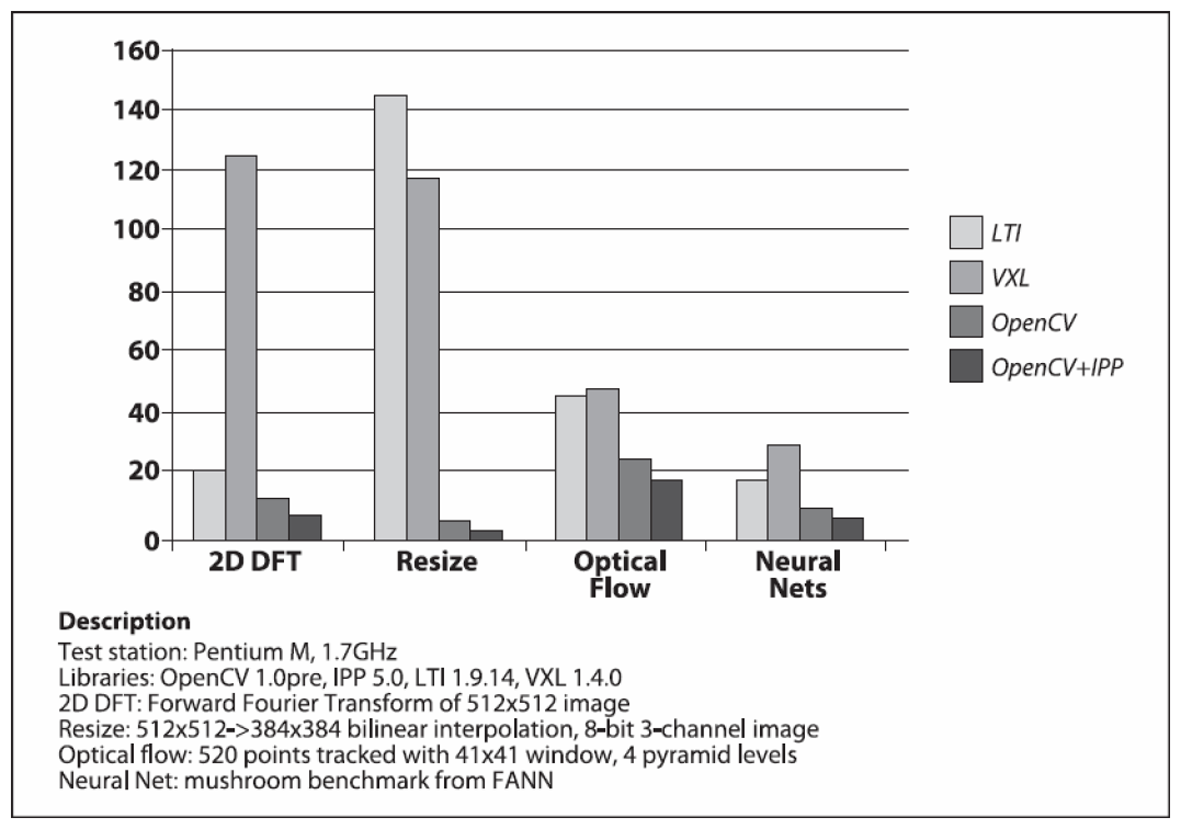
\includegraphics[width=100mm, keepaspectratio]{figures/opencv_speed.png}
\caption{Az OpenCV teljesítménye az LTI és VXL képfeldolgozási könyvtárakkal összehasonlítva.\\Forrás: \cite{opencv_book}}
\label{fig:opencv_speed}
\end{figure}

A teljes funkcionalitás részletekbe menő bemutatása -- mint láthattuk \cite{opencv_book} -- egy könyvet is megtölt, de a teljesség igénye nélkül tekintsük át, hogy milyen alapvető jellemzői és alkalmazásai vannak a környezetnek:

\begin{itemize}

 \item alap adatstruktúrák
  \begin{itemize}
   \item mátrixok, vektorok
  \end{itemize} 

 \item mátrix és vektor manipuláció, lineáris algebra
  
 \item dinamikus adatstruktúrák
  \begin{itemize}
   \item listák, sorok, halmazok
   \item gráfok és fák
  \end{itemize}

 \item kép és videó input/output
  \begin{itemize}
   \item beolvasás fájlból (kép vagy videó) és kameráról
   \item kiírási lehetőség képként vagy videóként
  \end{itemize}

 \item előfeldolgozás
  \begin{itemize}
   \item él- és sarokkeresés
   \item mintavételezés és interpoláció
   \item színkonverzió
   \item morfológiai operátorok
  \end{itemize}

 \item struktúraanalízis
  \begin{itemize}
   \item távolság- és Hough-transzformáció
   \item kontúrfeldolgozás
   \item sablonillesztés
   \item különböző momentumok
   \item Delaunay háromszögelés
  \end{itemize}

 \item kamerakalibráció
  \begin{itemize}
   \item kalibrációs mintázatok felismerése és követése
   \item fundamentális mátrix becslés
   \item homográfia becslés
   \item sztereó megfeleltetés
  \end{itemize}
  
 \item mozgásanalízis
  \begin{itemize}
   \item optical flow
   \item mozgásszegmentálás és -követés
  \end{itemize}

 \item objektumfelismerés
  \begin{itemize}
   \item eigen-módszerek
   \item rejtett Markov-modell (Hidden Markov Model -- HMM)
  \end{itemize}
  
  \item kiterjesztett valóság-támogatás (Augmented Reality -- AR)
  
  \item gépi tanulás könyvtár
  \begin{itemize}
    \item döntési fa-alapú tanulás
    \item klaszterezési algoritmusok (pl. k-szomszédság)
    \item neurális hálózatok
    \item Bayes-osztályozó
    \item szupport vektor gépek (Support Vector Machine -- SVM)
  \end{itemize}    
  
 \item GUI és rajzolás
  \begin{itemize}
   \item kép és videó megjelenítés
   \item billentyűzet és egérkezelés
   \item egyenes, kör, poligon, szöveg rajzolása
  \end{itemize}
  
\end{itemize}

Láthatjuk, hogy a fent felsorolt funkciókkal a gépi látás terén rengeteg egyszerűbb feladatot szinte ,,egy lépésben'', beépített, optimalizált eljárások segítségével oldhatunk meg. Ha nagyobb szabású projektbe kezdünk, akkor is hasznunkra lehet, hogy részben vagy egészében egy több tízezres felhasználói tábor (melynek jelentős részét aktív kutatók alkotják) visszajelzései alapján fejlesztett környezetre építhetjük munkánkat.

\bigskip

Az OpenCV régebbi verzióiban a számos előny mellett hátrányként volt megemlíthető, hogy segítségével a felhasználói felületet csak nagyon leegyszerűsített módon szabhattuk testre. Igaz, hogy a könyvtár feladata elsősorban a képfeldolgozás és nem a megjelenítés, így ebből a nézőpontból a beépített kép és videó megjelenítési lehetőség, billentyűzet- és egérkezelés valamint trackbarok (csúsztatható kezelőszerv értékek beállítására) létrehozásának lehetősége inkább hozzáadott értékként jelent meg, azonban ez nem változtat azon a tényen, hogy ha igény van felhasználóbarát kezelőfelület készítésére, az OpenCV-t mindenképpen integrálnunk kellett valamely elterjedt grafikus felhasználói felület toolkittel.

A 2.1-es verziótól kezdődően megjelent egy némileg fejlettebb \textbf{Qt alapú felhasználói felület}. Teljes szabadságot még ez sem ad a felületek kialakításában, de az egyszerűbb projektek kezelőszerveinek és megjelenítésének problémája már kielégítően elvégezhető egyéb eszköz használata nélkül.

%,,,,,,,,,,,,,,,,,,,,,,,,,,,,,,,,,,,,,,,,,,,,,,,,,,,,,,,,,,,,,,,,,,,,,,,,,,,,
\section{A Qt keretrendszer}\label{sect:qt}
%,,,,,,,,,,,,,,,,,,,,,,,,,,,,,,,,,,,,,,,,,,,,,,,,,,,,,,,,,,,,,,,,,,,,,,,,,,,,

A \textbf{Qt}\footnote{\url{http://qt.digia.com/}} (ejtsd az angol ,,cute'' szó mintájára: kjút) keretrendszer egy széles körben használt szoftver, amelyet egyrészt grafikus felhasználói felületek (Graphical User Interface -- GUI), másrészt parancssoros (Command Line Interface -- CLI) alkalmazások fejlesztésére is használnak. A grafikus felhasználói felületek fejlesztése során a Qt úgynevezett wiget-toolkitként funkcionál -- kis, önálló elemek (widgetek) felhasználását és összekötését teszi lehetővé, ezek összességéből áll össze az elkészült grafikus felület. A szoftver a  GPL~v3\footnote{\url{http://www.gnu.org/licenses/gpl.html}} illetve LGPL~v2\footnote{\url{http://www.gnu.org/licenses/lgpl-2.1.html}} licencek szerint szabadon elérhető. \cite{qt_wiki}

A keretrendszer egyik nagy előnyének számít más rendszerekkel összehasonlítva, hogy a grafikus felületek kirajzolásakor minden operációs rendszeren igyekszik az elérhető natív elemeket használni, ennek köszönhetően (a natív kirajzolásokból származó nagyszerű performancia mellett) a Qt-tal fejlesztett alkalmazások semelyik platformon nem tűnnek rendszeridegennek.

\bigskip

A Qt projekt első hivatalos kiadása a Nokia \emph{Qt Development Frameworks} csoport égisze alatt látta meg a napvilágot, miután a finn mobilgyártó felvásárolta a technológiát a norvég Trolltech vállalattól. Ennek megfelelően a kezdeti években az asztali platformok mellett leginkább a Symbian operációs rendszer támogatása jelentette a fő csapásirányt. A Nokia azonban 2011-ben szakított saját fejlesztésű operációs rendszerével, és a további bizalmát a Microsoft akkori és elkövetkező mobilplatformjaiba (Windows Phone~7, majd 8) fektette.

Ezt követően a Nokia megvált a rendszer kereskedelmi jogaitól, és azok a Digia\footnote{\url{http://www.digia.com/}} vállalathoz kerültek, amely azóta is a projekt karbantartója, bár a tényleges fejlesztői munka nagy részét továbbra is a Nokia mérnökei végzik. A tranzakció után az új tulajdonos közvetlen célnak tűzte ki, hogy aktualizálják a Qt által támogatott platformok listáját az időközben népszerűvé vált rendszerekkel.

A dolgozat írásakor támogatott fontosabb operációs rendszerek:

\begin{itemize}
  \item Windows (XP és 7)
  \item OS X
  \item Linux, FreeBSD, OpenBSD
  \item iOS
  \item Android
  \item QNX (BlackBerry 10)
\end{itemize}

A Qt-ot használó alkalmazások programozási nyelve alapvetően a sztenderd C++, a \emph{Meta Object Compiler} (moc) kódgenerátorral kiegészítve, amely számos beépített makróval teszi könnyebbé a fejlesztést. Több más programozási nyelv is használható az ún. \textbf{kötések} (bindings) használatával. A Qt~4-es verziójához elérhető kötések listája a teljesség igénye nélkül:

\begin{itemize}
  \item C\# és .NET
  \item Java
  \item Python
  \item szkriptnyelvek
  \begin{itemize}
    \item Perl
    \item Ruby
    \item PHP
    \item Tcl
  \end{itemize}    
   
\end{itemize}

A Qt a GUI események célba juttatását a \textbf{signals/slots} rendszer segítségével végzi. A módszer az \emph{Observer}\footnote{\url{http://en.wikipedia.org/wiki/Observer_pattern}} (Megfigyelő) tervezési minta megvalósítására nyújt egyszerű és szabványosított lehetőséget. A felhasználói felület elemei (widgetek) jelzéseket (signal) bocsátanak ki -- pl. ,,a X gombot megnyomták'', ,,a beviteli mező értéke Y-ra változott'' -- amelyeket más elemek ,,foglalataihoz'' (slot) köthetünk, ahol az eseményt lekezelhetjük. Látható, hogy ez a struktúra remekül illeszkedik a grafikus felhasználói felülete eseménykezelésére, de ezen kívül időzítések és értesítések kézbesítésére is alkalmas.

A signalok és slotok a megvalósításukat tekintve speciális  függvények, melyeket deklarálásukkor a két bekezdéssel előbb említett \emph{moc} (Meta Object Compiler) automatikusan generál, elkerülve ezzel a feleslegesen ismétlődő kódrészletek elburjánzását (boilerplate kód).

\bigskip

A Qt~4-es verziójához nagyjából 6 éven át érkeztek a kisebb/nagyobb frissítések, egészen a 4.8-as kiadásig. Ezt követően a koncepcionális változásokat hozó \textbf{Qt 5} fejlesztése folytatódik tovább. Az 5-ös verzió funkciói között között a hardveres gyorsítású megjelenítés, a QML\footnote{\url{http://en.wikipedia.org/wiki/QML}} és a JavaScript támogatása jelentik a legfontosabb újdonságokat.

A Qt~5 kiadásával a keretrendszer tett egy lépést a nyílt (open source) fejlesztés irányába: a \textbf{Qt~Project}\footnote{\url{http://qt-project.org/}} néven futó projektbe már külsős fejlesztők is delegálhatják javításaikat vagy új funkciókat, amelyeket a Digia és a Nokia csapata elbírál, és ha megfelelőnek találtatnak, bekerülhetnek a soron következő verzióba.

%............................................................................
\subsection{A Qt Creator fejlesztői környezet}\label{sect:qt_creator}
%............................................................................

A \textbf{Qt Creator} egy integrált fejlesztői környezet (Integreated Development Environment -- IDE) Qt alapú fejlesztésekhez. Használatával jelentősen megkönnyíthető mind a grafikus felületek kialakítása, mind az alkalmazások forráskódjának szerkesztése és fordítása. \cite{qtcreator_wiki}

\paragraph{Szerkesztő}

A kódszerkesztő (editor) a kor követelményeinek megfelelően támogatja a szintaxis-kiemelést valamint az automatikus kódkiegészítést (code completion) több programozási nyelvre is. A szerkesztő hátrányának róható fel, hogy a megnyitott fájlokat nem a manapság elterjedt fülek (tab) használatával rendezi, hanem saját fejlesztésű listát használ erre a célra, amely más fejlesztői környezetekből érkezve kissé idegen.

\paragraph{Qt Designer}

A felhasználó felületek kialakításában nélkülözhetetlen segítséget nyújt a beépített Qt Designer eszköz. Használatával WYSIWYG (What You See Is What You Get) módon végezhetjük az alkalmazás grafikus felületének kialakítását. Választhatunk a számtalan beépített widget közül, de saját elemek létrehozását is támogatja a rendszer -- a widgetek fejlesztési konvencióit betartva az egyedi elemek is grafikusan jelennek meg a szerkesztőfelületen.

A felületek integrálása a kóddal az \sectref{qt} szakaszban említett signal-slot mechanizmus segítségével történhet, amelynek megvalósítása szintén nagyon felhasználóbarát módon sikerült.

\paragraph{Qt Quick Designer}

Ez az eszköz animációk fejlesztésére szolgál, amelyeket QML\footnote{\url{http://en.wikipedia.org/wiki/QML}} nyelvű leírásukkal adhatunk meg. A Qt natívan támogatja a nagyfrekvenciás (60 FPS) animációk készítését és lejátszását, ezáltal a 2D vagy 3D animációk ,,simák'', akadás mentesek lehetnek.

\paragraph{Verziókezelő-integráció}

A fejlesztői környezet képes a legnépszerűbb verziókezelő rendszerek támogatására. A támogatott rendszerek között van a népszerű \emph{Git} valamint \emph{Subversion (SVN)}, de \emph{CVS}, \emph{Bazaar} vagy \emph{Mercurial} kódbázisunkat is kezelhetjük közvetlenül a Qt Creatorral.

\paragraph{Példakódok}

Az alkalmazás nyitóképernyőjén rögtön számtalan példaprogram fogadja a felhasználót. A példák százas nagyságrendben érhetők el, és a legegyszerűbb feladatoktól (,,Hello World'') az egészen összetettekig próbálják lefedni a fejlesztés során esetlegesen felmerülő problémákat.

Letöltésük nem igényel többet néhány kattintásnál, és integrált megoldás lévén a kód betöltődik a szerkesztőbe -- azonnal futtathatjuk és elkezdhetjük megérteni a működését. Maga az ötlet, és a megvalósítás is példaértékű lehet más fejlesztőkörnyezetek számára, igazi kincsesbányát jelent a Qt működésében elmélyedni kívánó fejlesztők számára.

%,,,,,,,,,,,,,,,,,,,,,,,,,,,,,,,,,,,,,,,,,,,,,,,,,,,,,,,,,,,,,,,,,,,,,,,,,,,,
\section{Fejkamera}\label{sect:infracam}
%,,,,,,,,,,,,,,,,,,,,,,,,,,,,,,,,,,,,,,,,,,,,,,,,,,,,,,,,,,,,,,,,,,,,,,,,,,,,

A tekintetkövető rendszer fejlesztése közben hardveres technológiai kérdések is felmerültek. A legfontosabb ilyen kérdés a pupillát követő kamera kiválasztása és elhelyezése volt.

%............................................................................
\subsection{Eszközök}\label{sect:infracam_eszkozok}
%............................................................................

Költséghatékonysági okokból -- ezzel együtt demonstrálandó, hogy nem feltétlenül kellenek speciális eszközök működőképes tekintetkövető összeállításához -- a TODO ábrán látható \textbf{6 LED-es webkamerát}\footnote{megvásárolható: \url{http://bit.ly/15yoLJ3}} választottam.

TODO kamera

A kamera gyártója ismeretlen (no-name), viszont jelen dolgozat írásának idején is mindössze 5 amerikai dollárért  -- 2013 májusi árfolyamon nagyjából 1\,200 forintos áron -- beszerezhető a lábjegyzetben szereplő hivatkozást meglátogatva.

A webkamera főbb paraméterei:

\begin{itemize}
  \item \textbf{videó mód:} színes, 24-bit 
  \item \textbf{érzékelő:} 1/4 CMOS
  \item \textbf{látószög:} 56$^{\circ}$
  \item \textbf{felbontás:} 640x480 képpont
  \item \textbf{képfrissítés:} 30 FPS
\end{itemize}

Az átlagos webkamerák között egyedi tulajdonsága, hogy a \textbf{lencséje cserélhető}, helyére bármilyen szabvány \emph{M12x0.5} (CCTV biztonsági kamerák körében elterjedt) foglalattal rendelkező lencse beilleszthető. Érdemes is megvásárolni a TODO ábrán látható \textbf{lencsekészletet}\footnote{megvásárolható: \url{http://bit.ly/17TtCCg}}, amely $2,\!8$-tól $16$ mm-es fókusztávig tartalmaz lencséket. A cserélhető lencséknek köszönhetően kiválaszthatjuk azt a fókusztávot, amely a kamera elhelyezésének függvényében a legjobb képet adja, azaz a szemrégió a lehető legjobban kitölti a képet.

TOOD lencsek

A webkamera nagy hátrányaként említhető meg, hogy működőképes meghajtóprogramot (driver) \textbf{csak Windows~7 rendszerre} lehetséges találni hozzá, azt is csak rengeteg keresgélés után. Az eszközt azonos külső mellett többféle vezérlővel forgalmazzák, ezek meghajtóprogramjai egymással nem kompatibilisek. Ha kamerához csomagolt CD elveszik, megsérül, vagy -- mint ahogyan sajnos a szerző esetében is előfordult -- egyáltalán nincs is a csomagban, ember legyen a talpán, aki megtalálja az eszközhöz tartozó drivert.

Azonban ha sikerül is, a kizárólagos \emph{Windows~7}-kompatibilitás miatt nem használhatjuk ki a \sectref{opencv} szakaszban bemutatott OpenCV, és a \sectref{qt} szakaszban bemutatott Qt cross-platform mivoltát.

%............................................................................
\subsection{Módosítások, elhelyezés}\label{sect:infracam_mod}
%............................................................................

Az előző szakaszban bemutatott webkamera specifikációi között nem tüntetik fel, így szerencsés véletlennek tekinthető, hogy a kamera -- valószínűsíthetően a gyártó költséghatékonysági törekvései miatt -- \textbf{nem tartalmaz infratükröt} a CMOS érzékelő elé építve.

Az infratükröt (amely nevéből adódóan visszaveri a beérkező infravörös tartománybeli fényt) a közép- illetve prémiumkategóriás webkamerák mindegyikébe beépítik, mivel használatával robusztusabb képminőség érhető el infrafényben gazdag megvilágítás esetén is.

A tükör hiányának jelen esetben viszont maximálisan pozitív következménye van: lehetőség nyílik a szemrégió infra-megvilágítására, amelynek előnyeit a \sectref{hw_optikai} szakaszban tárgyaltam.

\bigskip

A webkamera műanyag borítását leszerelve tudtam hozzáférni a nyomtatott áramkörhöz. A 6 db. LED-ből kettőt kiforrasztottam a helyéről, majd megfelelő fizikai méretekkel és elektronikai paraméterekkel rendelkező \textbf{infra LED-ekkel helyettesítettem} őket. Az új LED-ek beforrasztása és a kamera összeszerelése után a fennmaradó 4 normál LED-et letakartam, hogy fényük ne zavarja az infra-megvilágítást.

TODO osszehasonlito kep

A művelet elvégzése előtt és után készült képek a TODO ábrán láthatók. A várakozásaimnak megfelelően az infrafénnyel megvilágított szemrégió jóval kevésbé (gyakorlatilag elenyészően kis mértékben) érzékeny a látható fény tartományába eső megvilágítási egyenlőtlenségekkel, tükröződésekkel szemben. Igény szerint a kontraszt tovább növelhető a meglévő kettőnél több LED infrára cserélésével.

\bigskip

Végezetül a webkamera elhelyezéséről kellett gondoskodnom. A problémát úgy oldottam meg, hogy a kamerát egy bézbólsapka napellenzőjéhez rögzítettem a kamerán található csíptető segítségével, a kamera kábelét pedig több ponton a sapkához rögzítve hátrafelé elvezettem, majd a számítógéphez egy USB hosszabbítón keresztül csatlakoztattam. Az elkészült összeállítás a TODO ábrán látható.

TODO sapkas kep

Ebben az összeállításban a szem elé függesztett kamera a látótér meglehetősen nagy százalékát takarja ki, de a rendszer működését ez alapvetően nem befolyásolja, legfeljebb kis megszokást igényel. Bemutató célokra ez a kényelmetlenség elfogadható mértékű, emellett könnyen belátható, hogy speciálisan a feladatra szabott hardverrel a lencse--érzékelő--kamera hármas akár körömnyi területen is elhelyezhető lenne. Ugyanígy léteznek technológiák a jelenlegi kábeles összeköttetés vezeték nélküli kiváltására is.
%----------------------------------------------------------------------------
\chapter{Megvalósítás}\label{sect:hardver}
%----------------------------------------------------------------------------

A rendszer szoftverét C++ nyelven fejlesztettem, az OpenCV gépi látás könyvtár, illetve a Qt felhasználói toolkit segítségével. A feladat megoldása során törekedtem az objektum-orientált paradigma szem előtt tartására, valamint hogy az elkészült rendszer a lehető legkönnyebben testre szabható, illetve igény esetén kiegészíthető legyen.

%Szöveg.

%,,,,,,,,,,,,,,,,,,,,,,,,,,,,,,,,,,,,,,,,,,,,,,,,,,,,,,,,,,,,,,,,,,,,,,,,,,,,
\section{Az OpenCV könyvtár}\label{sect:opencv}
%,,,,,,,,,,,,,,,,,,,,,,,,,,,,,,,,,,,,,,,,,,,,,,,,,,,,,,,,,,,,,,,,,,,,,,,,,,,,

Az OpenCV\footnote{\url{http://opencv.willowgarage.com/}} egy nyílt forráskódú gépi látás (computer vision) könyvtár. Elsődleges célja, keretet nyújtani \textbf{valósidejű} képfeldolgozási alkalmazások fejlesztésére. A könyvtár szabadon letölthető és felhasználható a BSD licenc\footnote{\url{http://www.linfo.org/bsdlicense.html}} keretein belül.

\bigskip

Az OpenCV projekt hivatalosan 1999-ben indult az Intel kezdeményezésében. A nagyközönségnek a 2000. évi \textit{,,IEEE Conference on Computer Vision and Pattern Recognition''} konferencián mutatkozott be, majd öt béta-verziót követően 2006-ban jutott el az 1.0-ás hivatalos kiadásig. A fejlesztése itt úgy tűnt, hogy megáll, de végül a projektet a Willow Garage\footnote{\url{http://www.willowgarage.com/}} robotikai kutatólabor 2008-ban szárnyai alá vette, és azóta is aktív fejlesztés alatt áll. 2008 októberében az 1.1-es verzióval közel egy időben látott napvilágot az elsõ hivatalos OpenCV-vel foglalkozó könyv \textit{,,Learning OpenCV: Computer Vision with the OpenCV Library''} címmel Gary Bradski és Adrian Kaehler fejlesztõk tollából \cite{opencv_book}. Az egy évvel később, 2009 októberében megjelent 2.0-ás verzióval a projekt nagy fejlődésen esett át. Ebben a verzióban található meg elõször a C++ és Python interfész (ez a meglévő C mellett már három hivatalosan fejlesztett interfészt jelent), amely az egyszerûbb kezelhetõség, új függvények mellett a meglévő eljárások teljesítmény tekintetében -- különösen többmagos rendszereken -- jobb implementációját kínálja a felhasználóknak.

\bigskip

Az OpenCV jelenlegi 2.1-es verziója elérhető FreeBSD, Linux, Mac OS és Windows operációs rendszerek alá. Széles körben, mondhatni világszerte használt, felhasználói tábora több, mint 40\,000 főt számlál. Köszönhető ez többek között annak, hogy felhasználási lehetőségei igencsak sokrétűek: több, mint 500 optimalizált algoritmust kínál annak érdekében, hogy ,,ne kelljen újra feltalálnunk a kereket''. Sebesség tekintetében érződik a kipróbált, optimalizált algoritmusok használata: az OpenCV a jelenleg elérhető leggyorsabb alternatíva gépi látás terén (\figref{opencv_speed} ábra). Teljesítménye azonban adott esetben még tovább növelhető, mivel ha Intel IPP\footnote{\url{http://software.intel.com/en-us/intel-ipp/}} (Integrated Performance Primitives) támogatást észlel, az abban található szálakra optimalizált algoritmusok használatát fogja preferálni.

\begin{figure}[!ht]
\centering
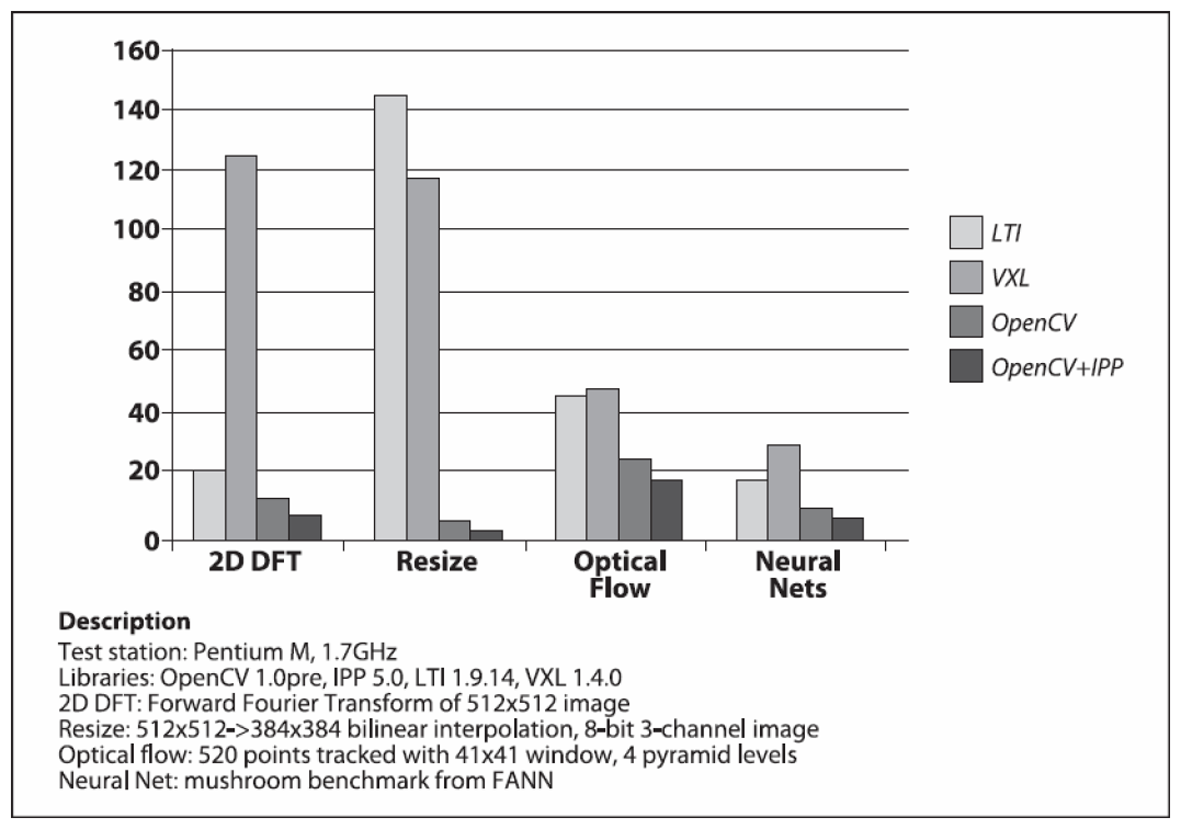
\includegraphics[width=100mm, keepaspectratio]{figures/opencv_speed.png}
\caption{Az OpenCV teljesítménye az LTI és VXL képfeldolgozási könyvtárakkal összehasonlítva.\\Forrás: \cite{opencv_book}}
\label{fig:opencv_speed}
\end{figure}

A teljes funkcionalitás részletekbe menõ bemutatása -- mint láthattuk \cite{opencv_book} -- egy könyvet is megtölt, de a teljesség igénye nélkül tekintsük át, hogy milyen alapvető jellemzői és alkalmazásai vannak a környezetnek:

\begin{itemize}

 \item alap adatstruktúrák
  \begin{itemize}
   \item mátrixok, vektorok
  \end{itemize} 

 \item mátrix és vektor manipuláció, lineáris algebra
  
 \item dinamikus adatstruktúrák
  \begin{itemize}
   \item listák, sorok, halmazok
   \item gráfok és fák
  \end{itemize}

 \item kép és videó input/output
  \begin{itemize}
   \item beolvasás fájlból (kép vagy videó) és kameráról
   \item kiírási lehetőség képként vagy videóként
  \end{itemize}

 \item előfeldolgozás
  \begin{itemize}
   \item él- és sarokkeresés
   \item mintavételezés és interpoláció
   \item színkonverzió
   \item morfológiai operátorok
  \end{itemize}

 \item struktúraanalízis
  \begin{itemize}
   \item távolság- és Hough-transzformáció
   \item kontúrfeldolgozás
   \item sablonillesztés
   \item különböző momentumok
   \item Delaunay háromszögelés
  \end{itemize}

 \item kamerakalibráció
  \begin{itemize}
   \item kalibrációs mintázatok felismerése és követése
   \item fundamentális mátrix becslés
   \item homográfia becslés
   \item sztereó megfeleltetés
  \end{itemize}
  
 \item mozgásanalízis
  \begin{itemize}
   \item optical flow
   \item mozgásszegmentálás és -követés
  \end{itemize}

 \item objektumfelismerés
  \begin{itemize}
   \item eigen-módszerek
   \item rejtett Markov-modell (Hidden Markov Model -- HMM)
  \end{itemize}
  
 \item GUI és rajzolás
  \begin{itemize}
   \item kép és videó megjelenítés
   \item billentyűzet és egérkezelés
   \item egyenes, kör, poligon, szöveg rajzolása
  \end{itemize}
  
\end{itemize}

Láthatjuk, hogy a fent felsorolt funkciókkal a gépi látás terén rengeteg egyszerűbb feladatot szinte ,,egy lépésben'', beépített, optimalizált eljárások segítségével oldhatunk meg. Ha nagyobb szabású projektbe kezdünk, akkor is hasznunkra lehet, hogy részben vagy egészében egy több tízezres felhasználói tábor (melynek jelentős részét aktív kutatók alkotják) visszajelzései alapján fejlesztett környezetre építhetjük munkánkat.

Az OpenCV számos előnye mellett hátrányként említhető meg, hogy segítségével a felhasználói felületet csak nagyon leegyszerűsített módon szabhatjuk testre. Igaz, hogy a könyvtár feladata elsősorban a képfeldolgozás és nem a megjelenítés, így ebből a nézőpontból a beépített kép és videó megjelenítési lehetőség, billentyűzet- és egérkezelés valamint trackbarok (csúsztatható kezelőszerv értékek beállítására) létrehozásának lehetősége inkább hozzáadott értékként jelenik meg. Azonban ez nem változtat azon a tényen, hogy ha igény van felhasználóbarát kezelőfelület készítésére, az OpenCV-t integrálnunk kell valamely elterjedt grafikus felhasználói felület toolkittel.

%,,,,,,,,,,,,,,,,,,,,,,,,,,,,,,,,,,,,,,,,,,,,,,,,,,,,,,,,,,,,,,,,,,,,,,,,,,,,
\section{Pszichológiai bemutató}\label{sect:pszicho}
%,,,,,,,,,,,,,,,,,,,,,,,,,,,,,,,,,,,,,,,,,,,,,,,,,,,,,,,,,,,,,,,,,,,,,,,,,,,,

A rendszer működését úgy demonstráltam, hogy végrehajtottam Alfred L. Yarbus orosz pszichológus 1967-es tanulmánya egy részletét. A kísérletben a kutatók azt bizonyították be, hogy a tesztalanyoknak előzetesen különböző kérdéseket feltéve, a kérdések jelentősen befolyásolták egy kép részleteinek vizsgálatát ahhoz képest, ha csak ,,szabadon'' nézegették azt. A teszteredményeket összefoglaló kép -- mint az egyik első a témával foglalkozó eredmény -- jól ismert a tekintetkövetéssel foglalkozók körében, ez látható a \figref{yarbus} ábrán.

\begin{figure}[!ht]
\centering
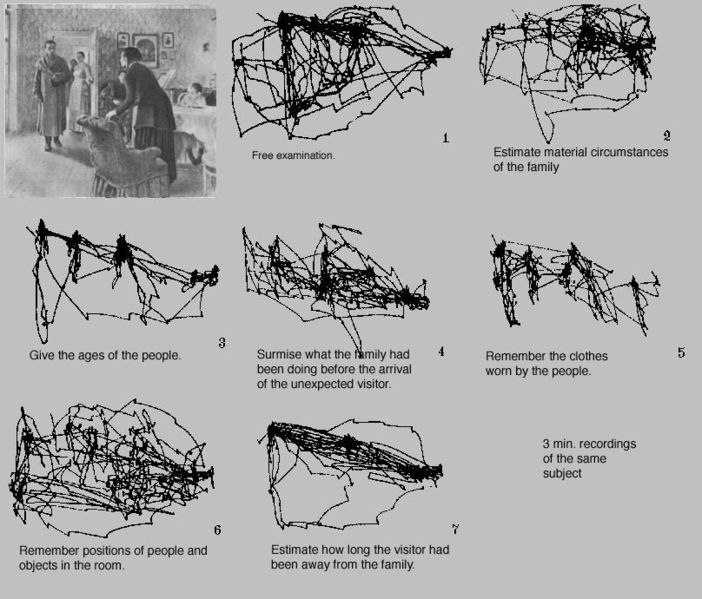
\includegraphics[width=140mm, keepaspectratio]{figures/yarbus.jpg}
\caption{Yarbus '67-es kísérletének eredménye}
\label{fig:yarbus}
\end{figure}

Látható, hogy a kísérlet végrehajtásához szükség volt a tekintet követésére. Ekkor még a kornak megfelelően nem álltak rendelkezésre kifinomult módszerek: az alanyokat egy meglehetősen kényelmetlen acélszerkezethez rögzítve vizsgálták. A bemutató alkalmazásomban arra kerestem a választ, hogy lehetséges-e hasonló méréseket elvégezni az általam fejlesztett rendszerrel.

\bigskip

Az általam tesztelt alanyoknak a következő kérdésekre kellett válaszolniuk a tesztkép (Repin: Váratlan utazó) rövid vizsgálata után. A vizsgálatot minden kérdésben 200 beérkezett érvényes mérési pontig folytattam, ez a felhasznált webkamera, illetve a feldolgozási sebesség mellett nagyjából kérdésenként 15--20 másodpercet vett igénybe.

\begin{enumerate}
 \item szabad nézelődés
 \item ,,Milyen anyagi körülmények között él a család?''
 \item ,,Adja meg az egyes szereplők életkorát!''
 \item ,,Mit csinálhattak a szereplők, mielőtt az utazó betoppant?''
 \item ,,Milyen ruhát viselnek a kép szereplői?''
 \item ,,Próbáljon megjegyezni minél több strukturális részletet (személyek, tárgyak pozíciója)!''
 \item ,,Mennyi ideig lehetett távol az utazó a családtól?''
\end{enumerate}

A kérdésekre nem volt jó, vagy rossz válasz, a kísérlet minden alanynál csak a feladatnak megfelelő figyelmi területek változását vizsgálja. A vizsgálatom eredménye a \label{fig:eredmeny} ábrán követhető.

\begin{figure}[!ht]
\centering
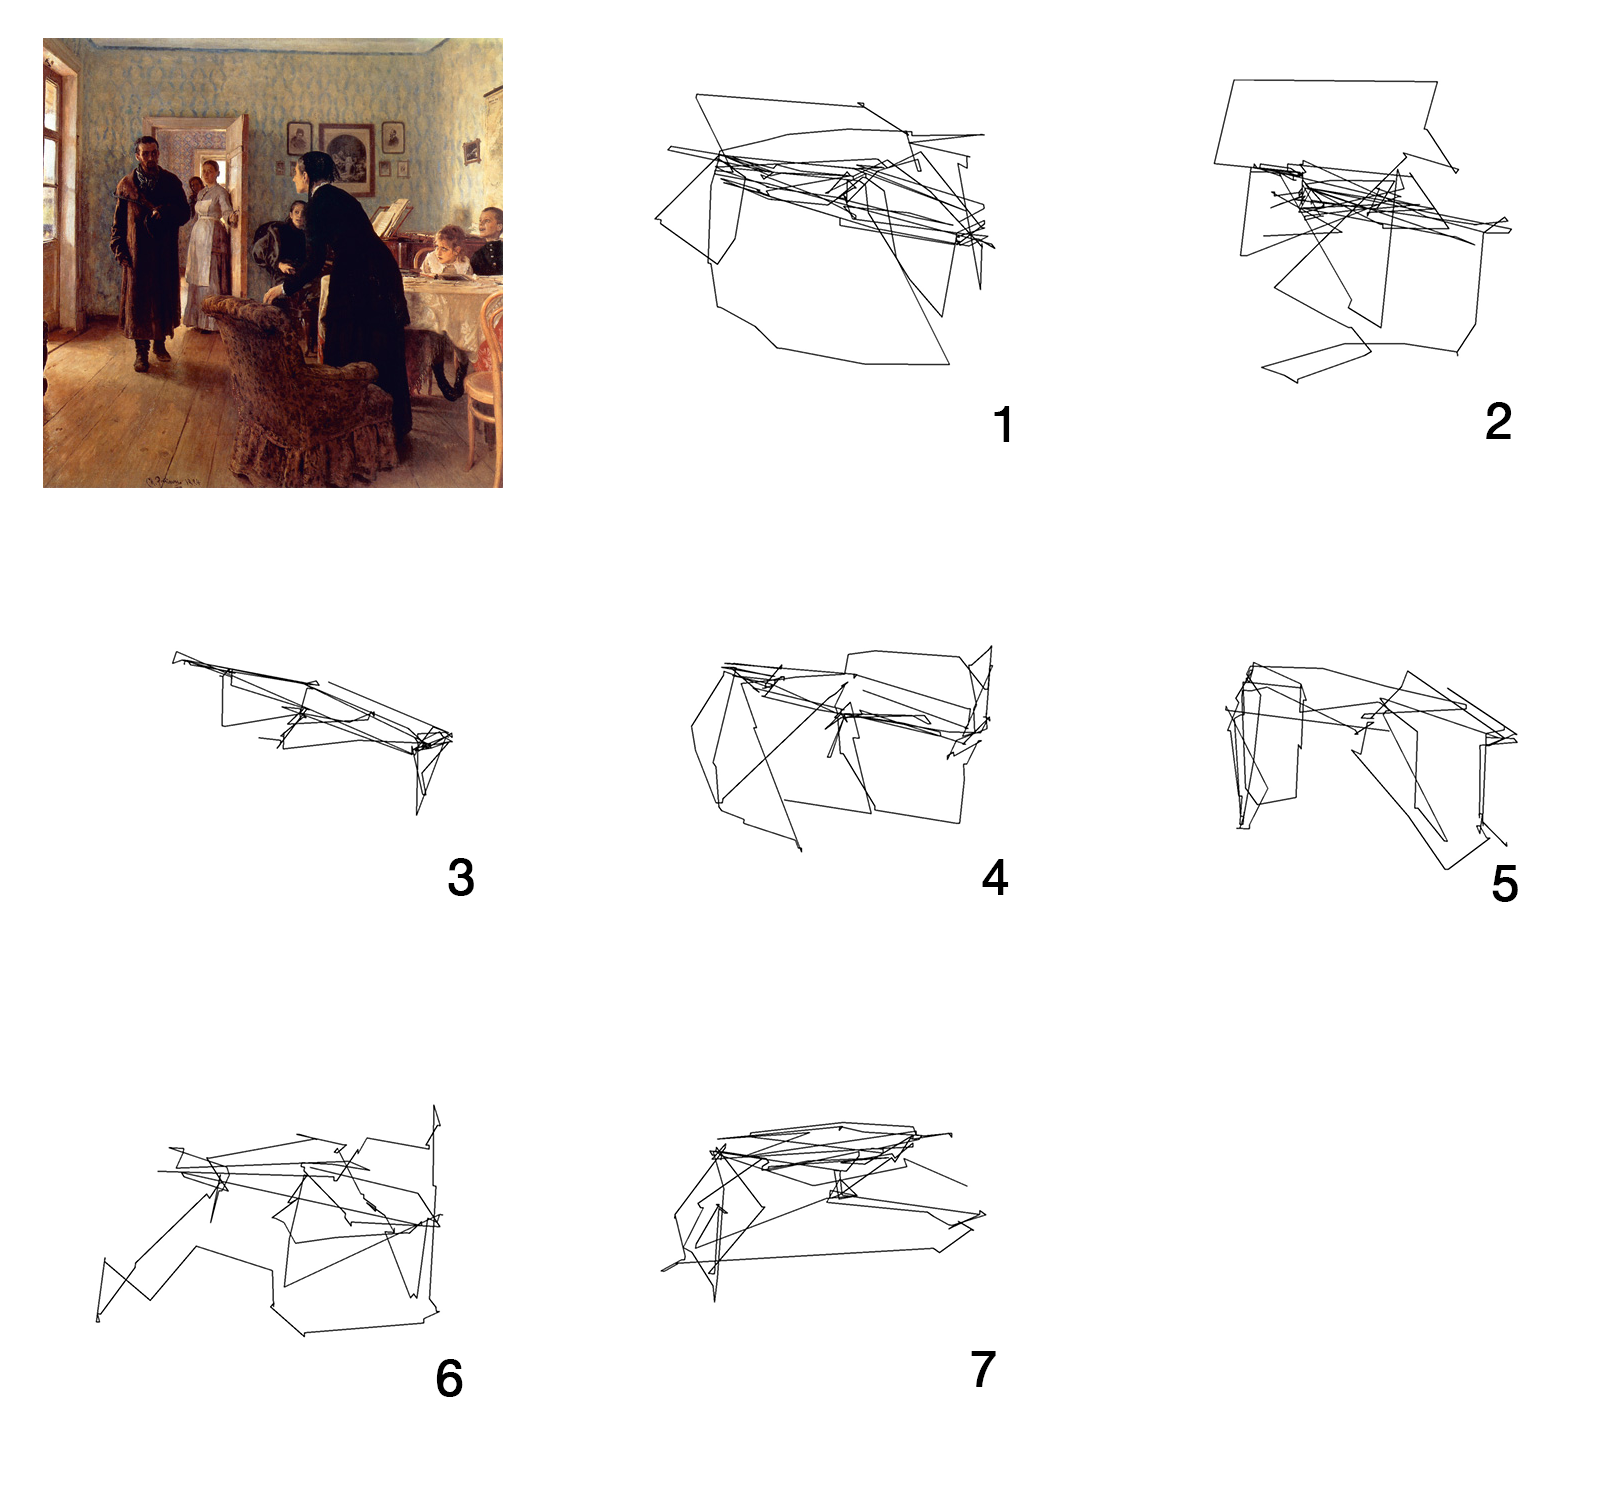
\includegraphics[width=140mm, keepaspectratio]{figures/yarbus_eredmeny.png}
\caption{Eredmények a saját rendszerrel}
\label{fig:eredmeny}
\end{figure}

Látható -- bár ez nem volt feltétel -- hogy a mérési eredmények ezen alany esetén meglehetősen jól fedik Yarbus tesztalanyának eredményeit. Az viszont mindenképpen kijelenthető, hogy szignifikáns különbség van az ábra első (szabad nézelődés), valamint többi része között. Nem célom a kísérlet pszichológiai eredményeit értékelni, az viszont bizonyos, hogy a rendszer hasonló kísérletek elvégzését támogatja.

%,,,,,,,,,,,,,,,,,,,,,,,,,,,,,,,,,,,,,,,,,,,,,,,,,,,,,,,,,,,,,,,,,,,,,,,,,,,,
\section{Webergonómiai bemutató}\label{sect:web}
%,,,,,,,,,,,,,,,,,,,,,,,,,,,,,,,,,,,,,,,,,,,,,,,,,,,,,,,,,,,,,,,,,,,,,,,,,,,,

Ahogyan dolgozatom első fejezetében már említettem, a tekintet követése a webergonómia területén is fontos kísérletek elvégzésére ad lehetőséget. A rendszer ilyen irányú képességeit demonstrálandó, elkészítettem az pszichológiai kísérlet adatait hőtérképen (heat map) megjelenítő funkciót is, ennek eredménye egy tesztképre a \label{fig:heatmap} ábrán látható.

\begin{figure}[!ht]
\centering
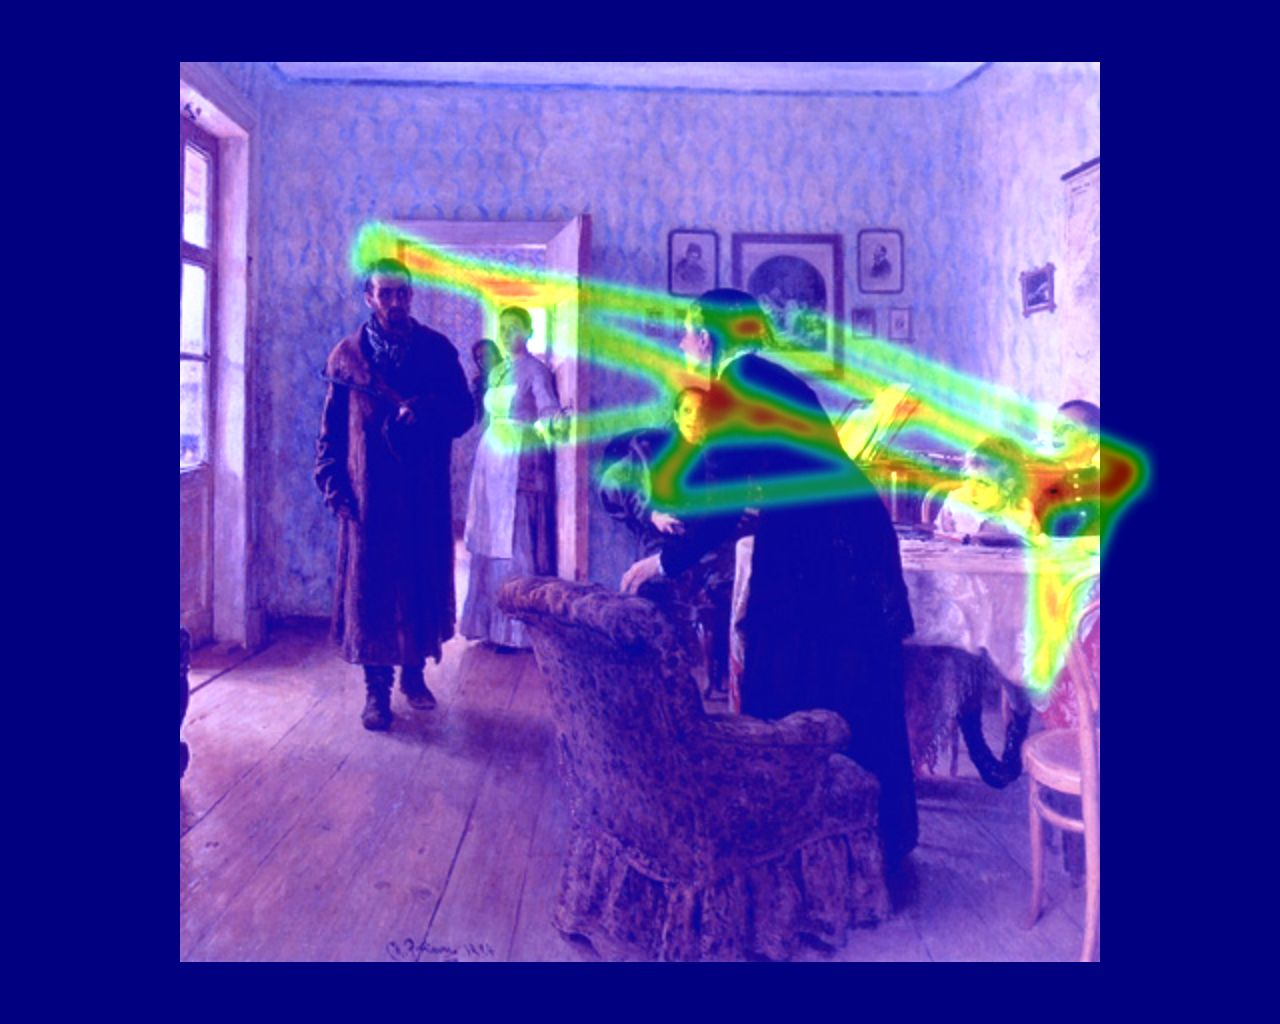
\includegraphics[width=100mm, keepaspectratio]{figures/heatmap.jpg}
\caption{Hőtérképes megjelenítés a pszichológiai teszt egy adathalmazára (,,Adja meg a szereplők életkorát!'')}
\label{fig:heatmap}
\end{figure}

Minden vizsgálatban célszerű a lehető leginkább informatív megjelenítést választani a rendelkezésre álló adathalmaz alapján. A képen egyre pirosabb színnel jelöltem a kép frekventáltan vizsgált területeit, például egy webergonómiai vizsgálatban az adatok effajta vizualizációja lehet a legcélszerűbb.

%............................................................................
%\subsection{Analóg TV-kamera}\label{sect:analog}
%............................................................................

%,,,,,,,,,,,,,,,,,,,,,,,,,,,,,,,,,,,,,,,,,,,,,,,,,,,,,,,,,,,,,,,,,,,,,,,,,,,,
%\section{Összefoglalás}\label{sect:hardver_osszefoglalas}
%,,,,,,,,,,,,,,,,,,,,,,,,,,,,,,,,,,,,,,,,,,,,,,,,,,,,,,,,,,,,,,,,,,,,,,,,,,,,

%Összefoglalás.
%----------------------------------------------------------------------------
\chapter{Megvalósítás}\label{sect:megvalositas}
%----------------------------------------------------------------------------

A megvalósítás során csak az \textbf{objektumorientált programozás} (object-oriented programming -- OOP) merült fel mint felhasználható módszertan. Az általánosan elterjedt koncepció lehetővé teszi egy komplex probléma kellően intuitív megfogalmazását és átlátható leírását. Erre a fejlesztés során szükség is volt, hiszen a meglehetősen összetetté váló programot csak gondos tervezéssel és kivitelezéssel lehetett megfelelő minőségben előállítani.

Az alkalmazás fejlesztését tehát az OOP paradigmáinak szem előtt tartásával végeztem. Az ismert alapelvek néhány szóban:

\begin{itemize}
  \item \textbf{absztrakció (abstraction):} a probléma valós világbeli objektumok mintájára történő modellezése, a lényegtelen részletek elhagyásával, a lényeges tulajdonságok kiemelésével
  \item \textbf{egységbe zárás (encapsulation):} az egyes osztályok és objektumpéldányok saját maguk rendelkezzenek a futások során szükséges adatok és metódusok felett
  \item \textbf{öröklődés (inheritance):} lehetséges egy általános ősosztály tetszőleges kiegészítése, specializálása a közös elemek megtartásával
  \item \textbf{polimorfizmus (polymorphism):} az egyes műveleteket képesek legyünk bemeneti paraméterek széles skáláján végrehajtani (metódus- vagy operátor-felüldefiniálás)
\end{itemize}

A fejezet \sectref{kovetelmenyek} szakaszában összefoglalom a feladat specifikációját, majd a \sectref{architektura} szakaszban részletesen dokumentálom a rendszer architektúrájával és implementációs részleteivel kapcsolatos tudnivalókat. A \sectref{gui} szakaszban a grafikus felhasználói felületet mutatom be, a \sectref{docs} szakasz pedig a felhasználói dokumentációnak ad helyet. A fejezet lezárásaként a \sectref{teszteles} szakaszban a rendszer kipróbálása során megfigyelt eredményeket és általános tapasztalatokat foglalom össze.

%,,,,,,,,,,,,,,,,,,,,,,,,,,,,,,,,,,,,,,,,,,,,,,,,,,,,,,,,,,,,,,,,,,,,,,,,,,,,
\section{Követelmények}\label{sect:kovetelmenyek}
%,,,,,,,,,,,,,,,,,,,,,,,,,,,,,,,,,,,,,,,,,,,,,,,,,,,,,,,,,,,,,,,,,,,,,,,,,,,,

Mielőtt a fejezet későbbi szakaszaiban részletekbe menőben bemutatom az elkészült alkalmazás architektúráját, illetve osztályainak pontos működését, szeretném dokumentálni a kész programra vonatkozó \textbf{követelményeket, azaz specifikációt}.

\bigskip

Az alkalmazás legyen képes:

\begin{enumerate}[a)]
  \item valósidejű \textbf{videofolyamot} olvasni a számítógépre kötött webkameráról (lásd \sectref{infracam} szakasz)
  \item a videofolyam feldolgozásával a \textbf{pupillapozíció meghatározására} a \sectref{pupillakov} szakaszban leírtak szerint.
  \item a tekintet \textbf{kalibrációjára} a \sectref{kalibracio} szakaszban ismertetett módszer felhasználásával.
  \item \textbf{munkamenetek} (session) rögzítésére a képernyő tartalmának mentésével együtt.
  \item a korábbi munkamenetek listázására, törlésére.
  \item munkamenetek \textbf{visszajátszására}.
  \item a munkamenetek alapján \textbf{hőtérképek} generálására (lásd \sectref{web} szakasz)
\end{enumerate}

%,,,,,,,,,,,,,,,,,,,,,,,,,,,,,,,,,,,,,,,,,,,,,,,,,,,,,,,,,,,,,,,,,,,,,,,,,,,,
\section{Architektúra}\label{sect:architektura}
%,,,,,,,,,,,,,,,,,,,,,,,,,,,,,,,,,,,,,,,,,,,,,,,,,,,,,,,,,,,,,,,,,,,,,,,,,,,,
  
  Az implementációt a \sectref{technologia} fejezetben bemutatott technológiák (OpenCV, Qt, Qt Creator) felhasználásával \textbf{C++ nyelven készítettem el} a Model--View--Controller (MVC) tervezési minta szem előtt tartásával. A kialakított osztályhierarchia a \figref{overview} ábrán látható módon épül fel. A kibővített osztálydiagram  -- a fontos változók és funkciók feltüntetésével -- megtalálható az \sectref{osztalydiagram} függelékben.
  
  Az átláthatóság kedvéért még a kibővített diagramról is lehagytam a kevésbé fontos tagváltozókat, és a nyilvánvaló funkcióval rendelkező függvényeket (pl. ,,getter'' vagy ,,setter'' metódusok). Emellett természetesen az információrejtés (information hiding) alapelvének megfelelően a tagváltozók amikor csak szükséges, privát változóként deklaráltak, és publikus interfész áll rendelkezésre az értékük lekérdezésére, vagy az értékadásra.

\begin{figure}[!ht]
\centering
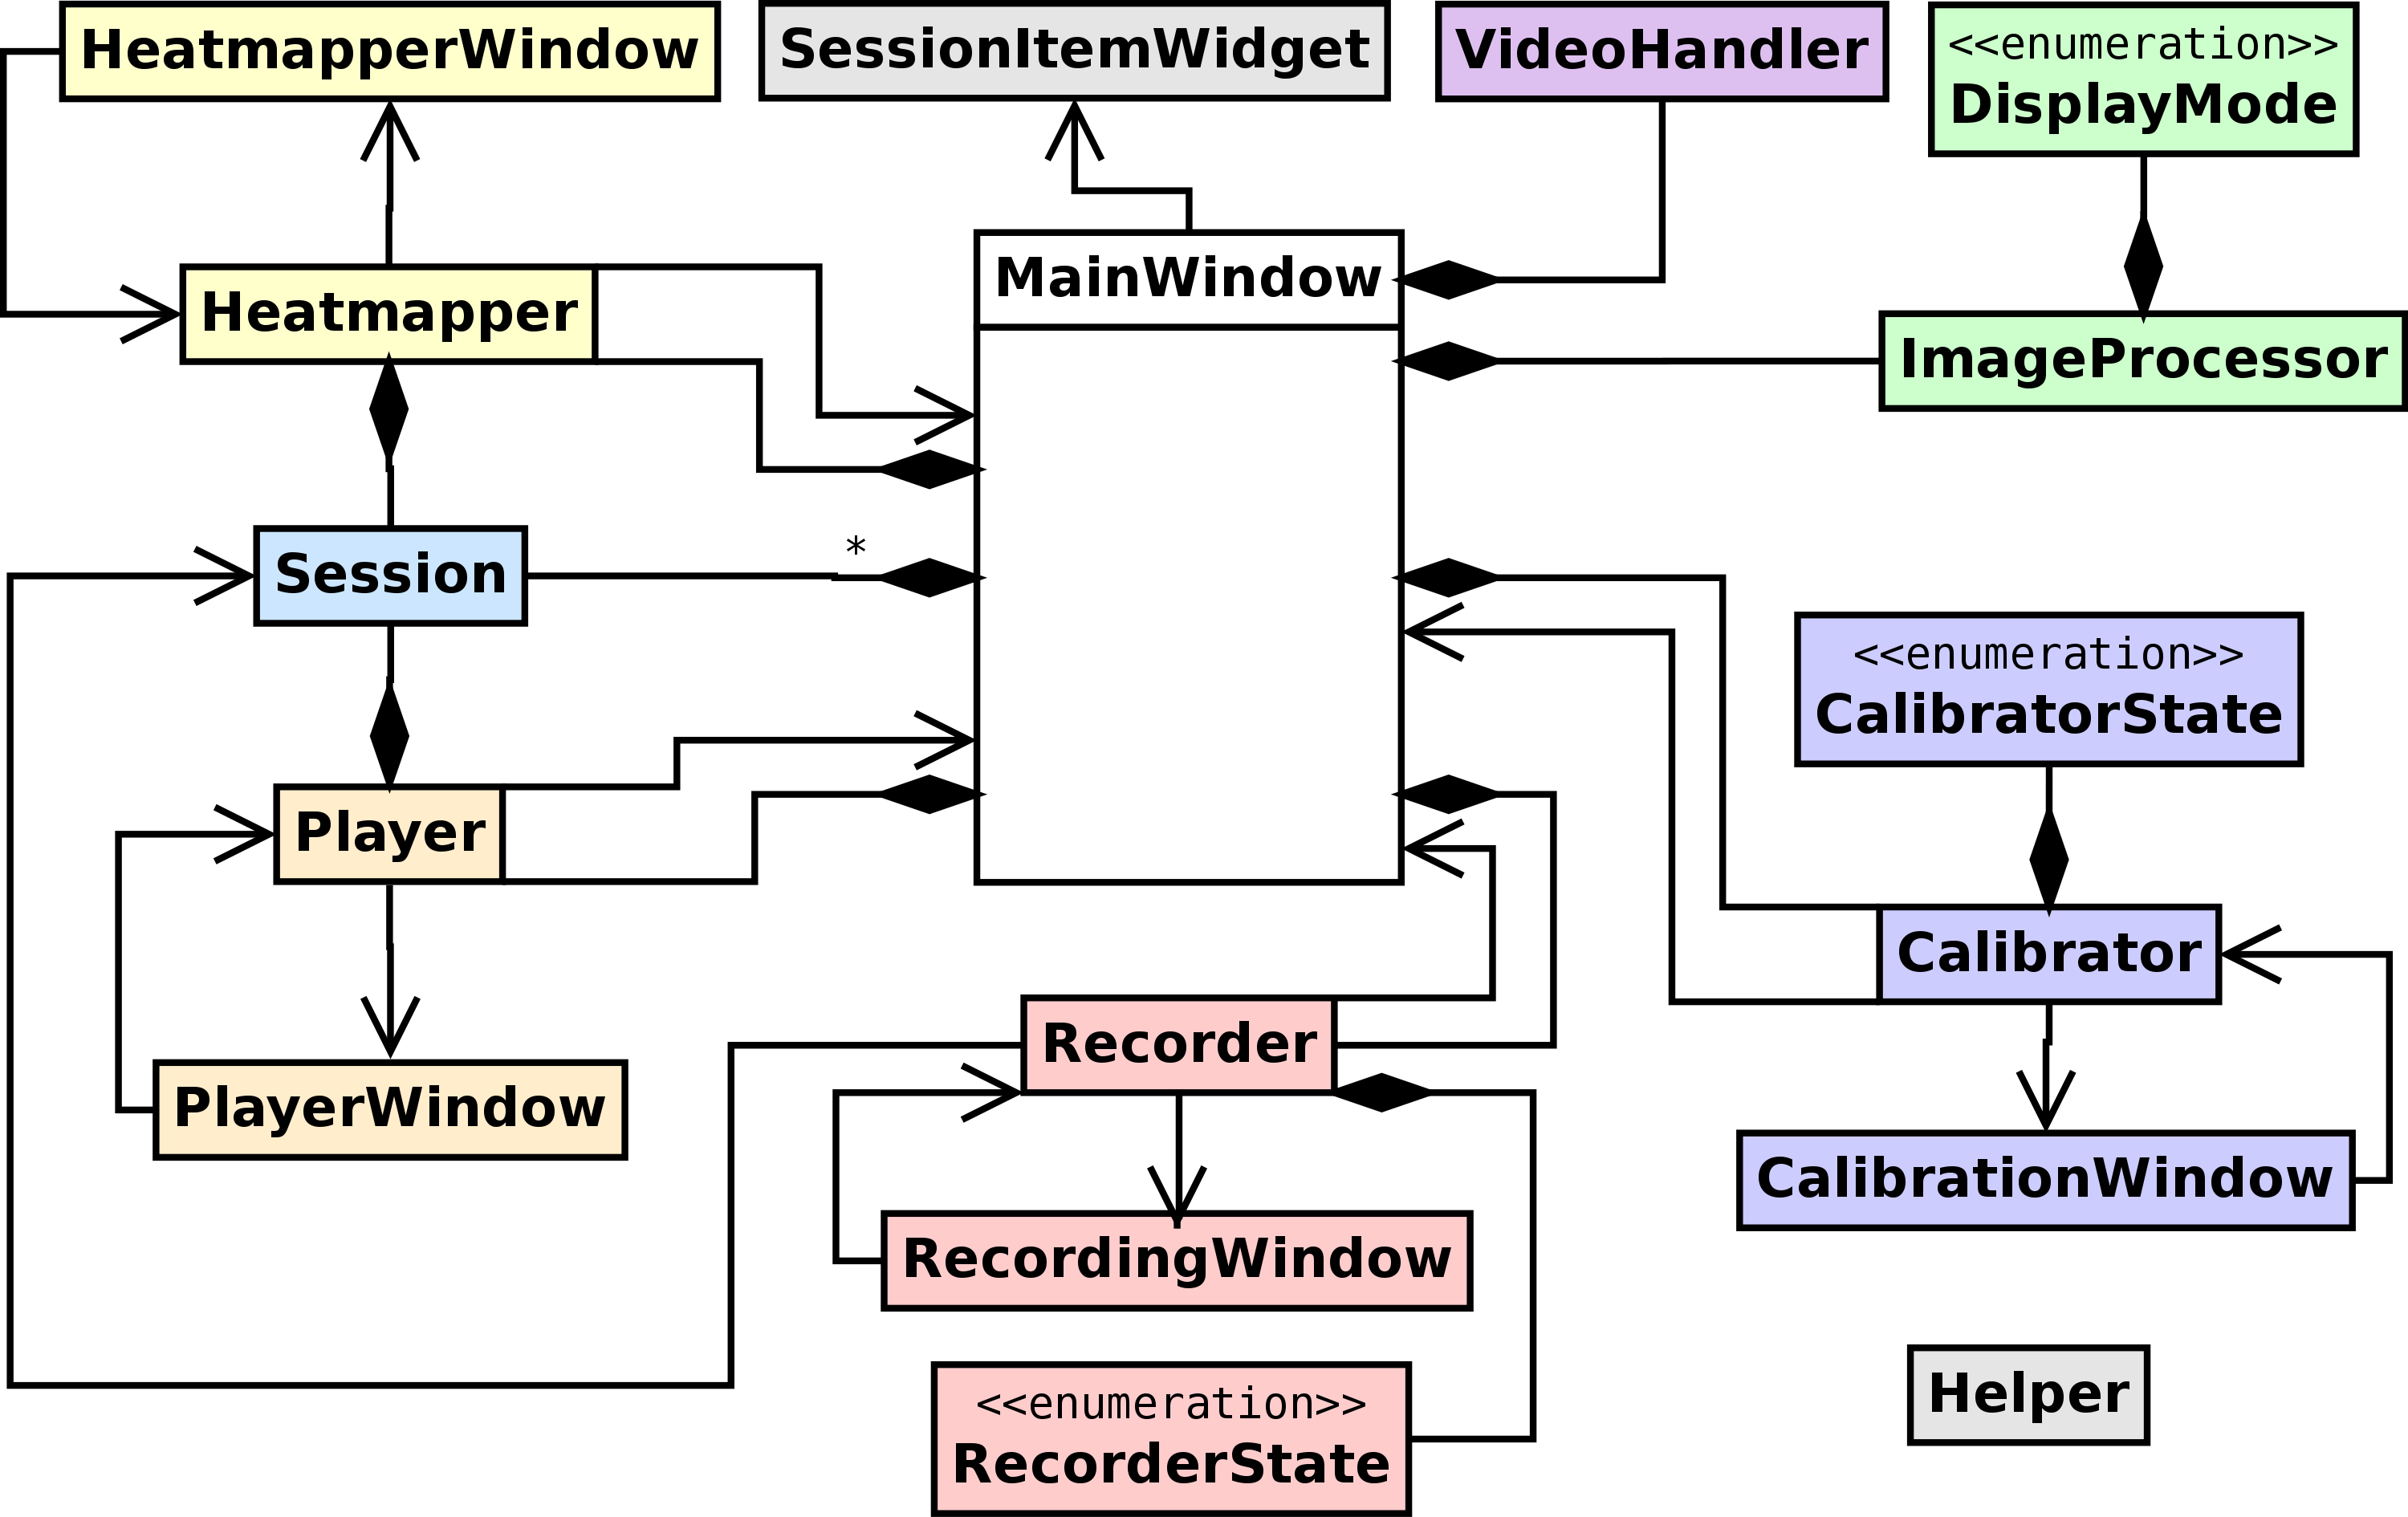
\includegraphics[width=140mm, keepaspectratio]{figures/overview_aa.png}
\caption{Az alkalmazás osztályhierarchiája}
\label{fig:overview}
\end{figure}

Az alkalmazás egyes funkcióit a videofolyam feldolgozásától egészen a hőtérképek generálásáig osztályok egy-egy csoportja végzi. A \figref{overview} ábrán színkódokkal jelöltem a logikailag összetartozó osztályokat. A specifikáció egyes pontjait kielégítő osztályok az ábráról leolvasva, felsorolás szintjén:

\begin{itemize}
  \item \texttt{MainWindow} -- az alkalmazás főablakát tartalmazó osztály, valamint ez szolgál általános kontrollerként is, lévén a felhasználói interakciók döntő része ide fut be
  \item \texttt{VideoHandler} -- a webkameráról beérkező videofolyam olvasásáért felelős
  \item \texttt{ImageProcessor} -- a képkockák feldolgozását -- a pupillakeresést -- végzi
  \item \texttt{Calibrator} -- a kalibrációt, majd kalibrált állapotban a \emph{pupilla-pozíció} $\Longrightarrow$ \emph{képernyő-pozíció} átszámítást végzi
  \item \texttt{Recorder} -- a munkamenetek rögzítését végzi
  \item \texttt{Player} -- a felvett munkamenetek visszajátszását teszi lehetővé ez az osztály
  \item \texttt{Heatmapper} -- a hőtérképek generálása történik ebben az osztályban
  \item \texttt{Session} -- konténerosztály egy-egy munkamenet futásidejű tárolása számára
  \item kisegítő osztályok
\end{itemize}

A továbbiakban sorra veszem az egyes osztályok interfészét, valamint belső működésüket, kicsit mélyebb betekintést engedve a felépítésükbe, egymással való összeköttetésükbe, valamint az esetleg érdekesnek ítélhető implementációs részletekbe.

%............................................................................
\subsection{A \texttt{MainWindow} osztály}\label{sect:mainwindow}
%............................................................................

\begin{figure}[!ht]
\centering
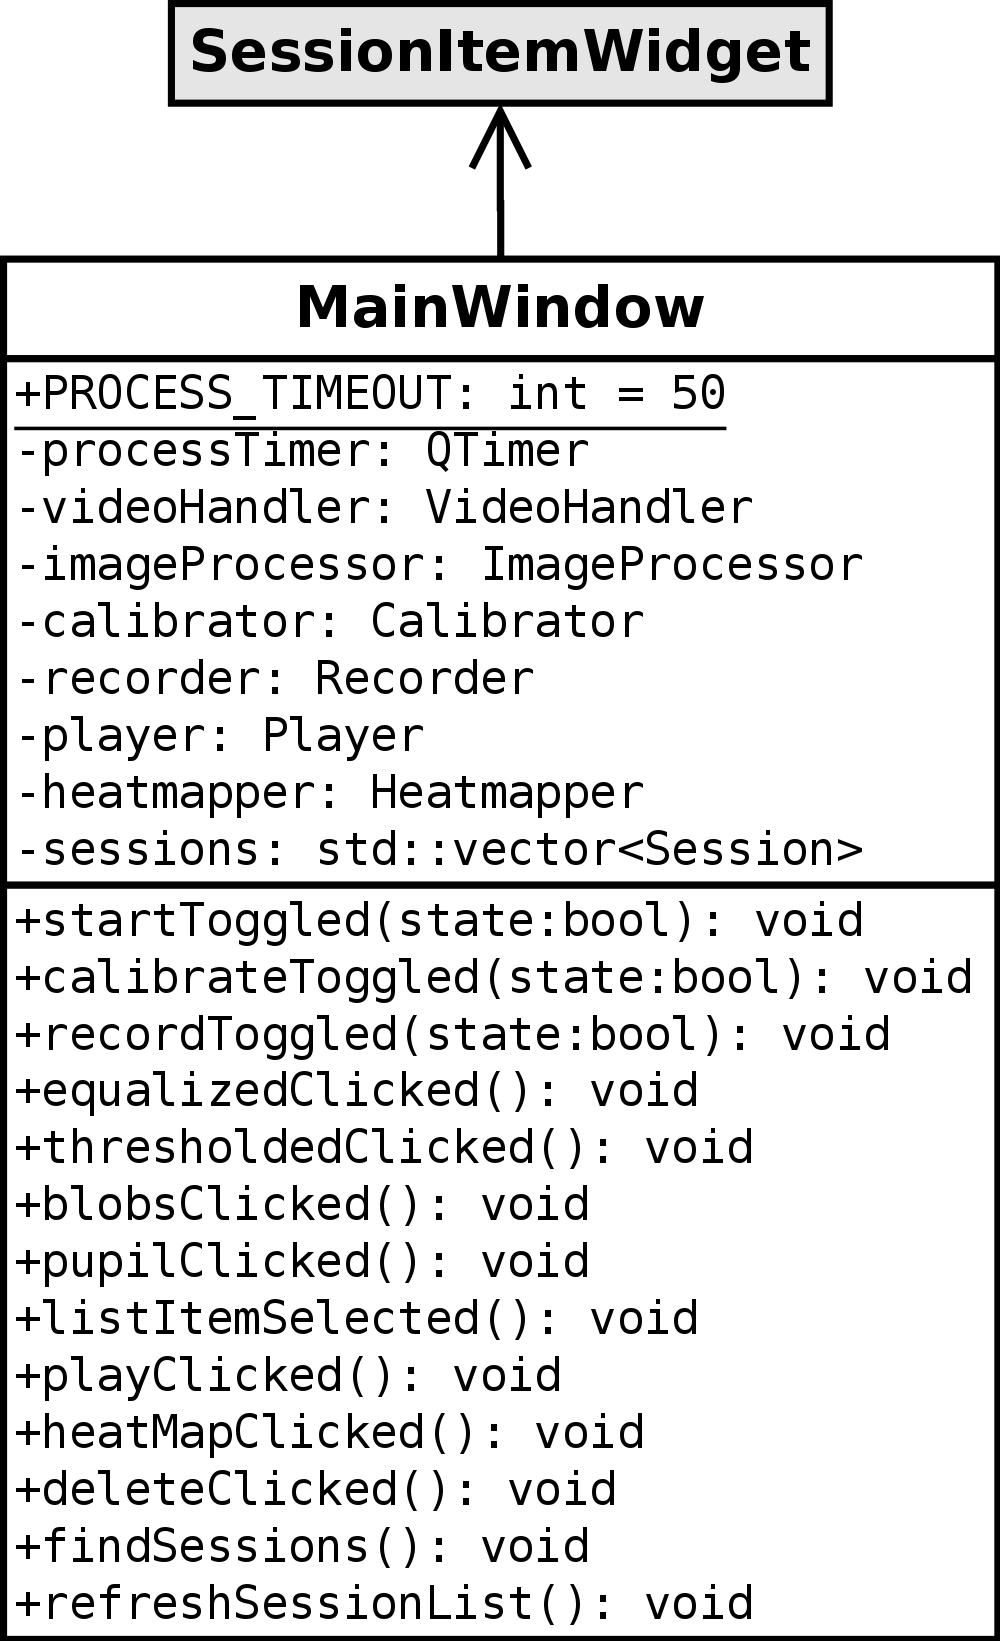
\includegraphics[width=50mm, keepaspectratio]{figures/class_mainwindow.png}
\end{figure}

A \texttt{MainWindow} osztály az alkalmazás általános kontrollereként működik. A nevéből is látszik, hogy ehhez az osztályhoz tartozik a program fő interfészablaka, ennek megfelelően a felhasználói interakciók lekezelése ezen osztály slotjaiban történik. Az osztályban tényleges feldolgozás nem történik, csak összefogja az egyes lépéseket elvégezni hivatott objektumokat, valamit biztosítja, hogy a felhasználói felület állapota mindig a program tényleges belső állapotát reprezentálja, és csak engedélyezett állapotátmenetek történhessenek.

\bigskip

Az \texttt{int PROCESS\_TIMEOUT} attribútum a \texttt{QTimer processTimer} időzítővel együtt a feldolgozás rögzített sebességgel történő elvégzését vezérli. Az előbbi ezredmásodpercben megadott értéke alapján hívódik a feldolgozást vezérlő \texttt{processTimeout} függvény.

A \texttt{sessions} lista az elmentett munkamenetek futásidejű tárolására szolgál, amely listát a \texttt{refreshSessionList} függvény állítja elő.

A \texttt{videoHandler}, \texttt{imageProcessor}, \texttt{calibrator}, \texttt{recorder}, \texttt{player} és \texttt{heatmapper} attribútumok tárolják a névből adódó típusú objektumpéldányokat, amelyek az alkalmazás egyes funkcióit valósítják meg.

A metódusok közül a \texttt{startToggled}, \texttt{calibrateToggled} és \texttt{recordToggled} metódusok sorra a videofolyam, kalibráció és a felvétel ki/bekapcsolását kezelik le.

A lejátszás során megjelenítési módok váltását kezelik le az \texttt{equalizedClicked} és a \texttt{pupilClicked} között felsorolt függvények.

%............................................................................
\subsection{A \texttt{VideoHandler} osztály}\label{sect:videohandler}
%............................................................................

\begin{figure}[!ht]
\centering
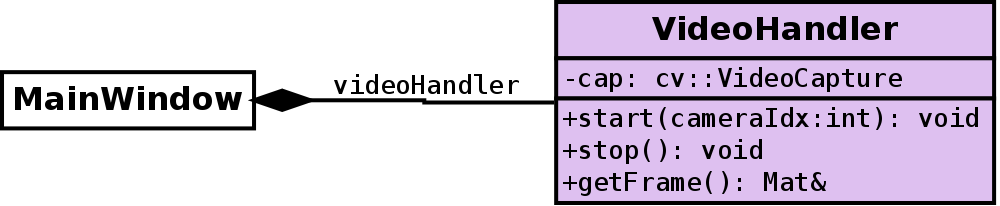
\includegraphics[width=80mm, keepaspectratio]{figures/class_videohandler.png}
\end{figure}

A \texttt{VideoHandler} az ,,alacsony szintű'' videokezelést végzi. A gyakorlatban ez úgy valósul meg, hogy \texttt{cv::VideoCapture cap} attribútumaként tartalmazza az OpenCV kamerakép-feldolgozásra szolgáló objektumának egy példányát.

A \texttt{start} függvényét egy kameraindexszel paraméterezve inicializálhatjuk a fent említett objektumot, a \texttt{stop} függvény pedig a kamera szabályos leállítására szolgál.

Elindított állapotban a \texttt{getFrame} függvénnyel kérhetjük le az adott pillanatban a kamera által érzékelt képet. A képet tartalmazó \texttt{cv::Mat} objektumpéldány szintén az osztály egy tagváltozójában kerül tárolásra, a \texttt{getFrame} függvény erre az objektumra mutató referenciát ad vissza. A megoldásnak nyilvánvalóan performanciabeli okai vannak: a tényleges objektumpéldány átadása felesleges számításokat róna a feldolgozási sorra.

%............................................................................
\subsection{Az \texttt{ImageProcessor} osztály}\label{sect:imageprocessor}
%............................................................................

\begin{figure}[!ht]
\centering
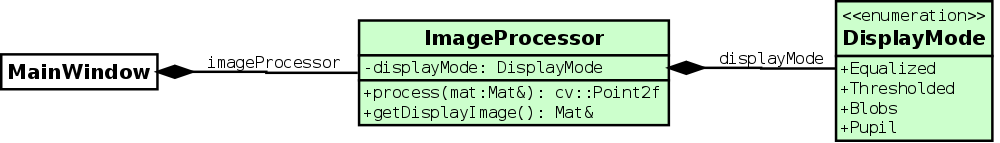
\includegraphics[width=140mm, keepaspectratio]{figures/class_imageprocessor.png}
\end{figure}

Az \texttt{ImageProcessor} osztály végzi a képkockák feldolgozását, és a pupilla azonosítását. A pupillakeresést az alkalmazás előfeldolgozás után blobok detektálásával és változatos szűrésével végzi, a \sectref{pupillakov} szakaszban részletesen bemutatott módon.

A \texttt{process} függvény végzi a felismerés, és a képen megtalált pupillaközépponttal tér vissza egy \texttt{cv::Point2f} változó használatával. A visszaadott középpont az érvénytelen $(-1, -1)$ koordinátákat kapja, ha nem sikerült a pupilla azonosítása.

Szükség van még ezen kívül a feldolgozás valamely közbülső állapotának képét lekérésére, ezt tehetjük meg a \texttt{getDisplayImage} metódus használatával. A függvény az \texttt{ImageProcessor} belső \texttt{displayMode} állapotának megfelelően adja vissza a kívánt képet. Fontos megjegyezni, hogy mindez csak a megjelenítést befolyásolja. A \texttt{displayMode} állapottól függetlenül a pupillafelismerés folyamata minden esetben elejétől a végéig lefut, majd visszatér a megtalált pupillaközéppont koordinátáival.
 
%............................................................................
\subsection{A \texttt{Calibrator} osztály}\label{sect:calibrator}
%............................................................................

\begin{figure}[!ht]
\centering
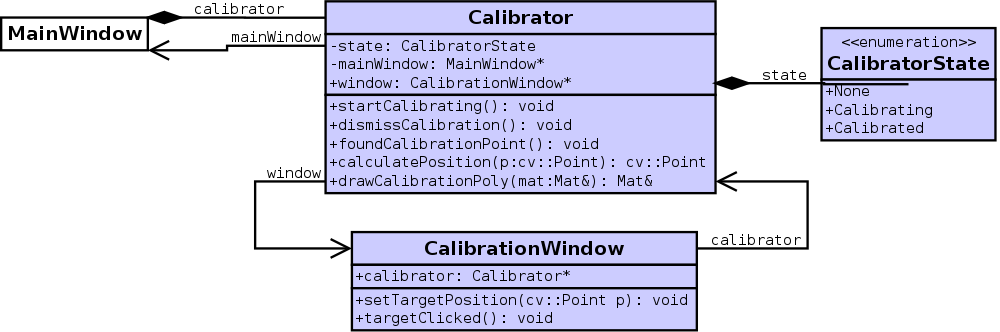
\includegraphics[width=140mm, keepaspectratio]{figures/class_calibrator.png}
\end{figure}

A \texttt{Calibrator} osztály az alkalmazás kalibrálását, majd a pupilla-koordináta alapján a képernyőn éppen nézett pont koordinátájának kiszámítását végzi. A kalibráció folyamatát részletesen a \sectref{kalibracio} szakaszban ismertettem.

Az osztályhoz tartozik egy \texttt{CalibrationWindow} objektum is, amely a futás során dinamikusan kerül lefoglalásra (ezért csak a rámutato pointert tároljuk). Emellett a kalibrálás állapotát is nyilvántartjuk, erre szolgálnak a \texttt{CalibratorState} felsorolás (enumeration) értékei: nincs kalibrálva (\texttt{None}), kalibrálás alatt (\texttt{Calibrating}), vagy kalibrálva (\texttt{Calibrated}).

\bigskip

A \texttt{startCalibrating} és \texttt{dismissCalibration} függvények elnevezései magukért beszélnek. A \texttt{dismissCalibration} függvény elveti a meglévő kalibrációs paramétereket, a \texttt{startCalibrating} metódus esetében pedig új kalibrációt indítunk: megnyílik a \texttt{CalibratorWindow} osztály felhasználói felülete (teljes képernyős kalibrációs ablak), rajta az első kalibrációs ponttal.

A kalibrációs ablakban tekintetünket az aktuális pontra irányítva, majd kattintva (\texttt{targetClicked}) a \texttt{foundCalibrationPoint} függvény hívása történik meg, amelyben utasításra kerül a következő kalibrációs pont kirajzolása \texttt{setTargetPosition}, vagy az utolsó pont esetén a kalibráció lezárása.

\bigskip

Kalibrált állapotban a \texttt{calculatePosition} függvény a \texttt{cv::Point} formában paraméterül adott pupillakoordinátát képzi le a kalibrációs paraméterek felhasználásával képernyő-koordinátákba.

\bigskip

Az \texttt{ImageProcessor} osztályhoz hasonlóan itt is az interfész részét képezik olyan metódusok, amelyek nem feltétlenül a tekintetkövetés szempontjából elengedhetetlen számítási feladatokat végeznek, csak a megjelenítés miatt van szükség rájuk. A \texttt{Calibrator} osztály esetében ilyen a \texttt{drawCalibrationPoly} függvény, amely a paraméteréül kapott képre egyszerűen rárajzolja a kalibrációs pontok négyszögét.

%............................................................................
\subsection{A \texttt{Session} osztály}\label{sect:session}
%............................................................................

\begin{figure}[!ht]
\centering
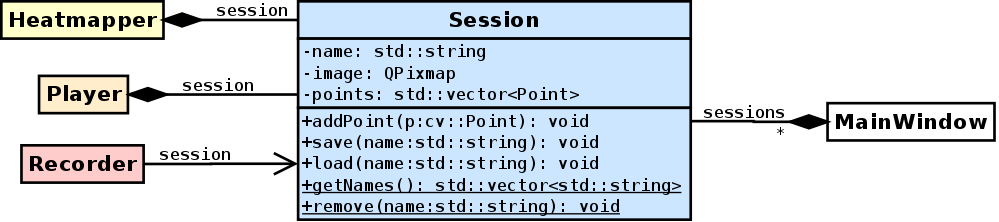
\includegraphics[width=140mm, keepaspectratio]{figures/class_session.png}
\end{figure}

A \texttt{Session} osztály az éppen felvétel alatt lévő, és már felvett munkamenetek futás közbeni tárolására szolgál.

Tagváltozóként tartalmazza a munkameneteket jellemző tulajdonságokat: a munkamenet nevét (azonosítóját, tetszőleges \texttt{std::string name}, a képet, amelyet a felvétel alatt az alany vizsgál (\texttt{QPixmap} objektumként), valamint a vizsgálat alatt felvett képernyő-koordinátákat (\texttt{std::vector<cv::Point> points} listaként).

\bigskip

A publikus interfészen keresztül lehetőség van a munkamenet-objektum lementésére a \texttt{save} metódus használatával. A paraméterül adott azonosítóval kerül lementésre a munkamenet, a futtatási könyvtár \texttt{session\_<név>} formátumú alkönyvtárába. A munkamenet alkönyvtárán belül létrejön a \texttt{bg.png} képfájl, ami értelemszerűen a vizsgálat alatt használt képet tartalmazza, valamint a \texttt{points.txt} szöveges fájl, amely  soronként tartalmazza a rögzített pontok képernyő-koordinátáit.

A mentés párjaként a \texttt{load} függvény tölti be a paraméterül kapott névvel lementett munkamenetet.

\bigskip

A fentieken kívül két statikus metódus is helyet kapott a \texttt{Session} osztályban. A \texttt{getNames} függvény a már lementett munkamenetek neveinek tömbjét adja vissza, a \texttt{remove} osztálymetódus pedig visszavonhatatlanul törli a háttértárról paraméterként megadott névvel rendelkező munkamenetet.

%............................................................................
\subsection{A \texttt{Recorder} osztály}\label{sect:recorder}
%............................................................................

\begin{figure}[!ht]
\centering
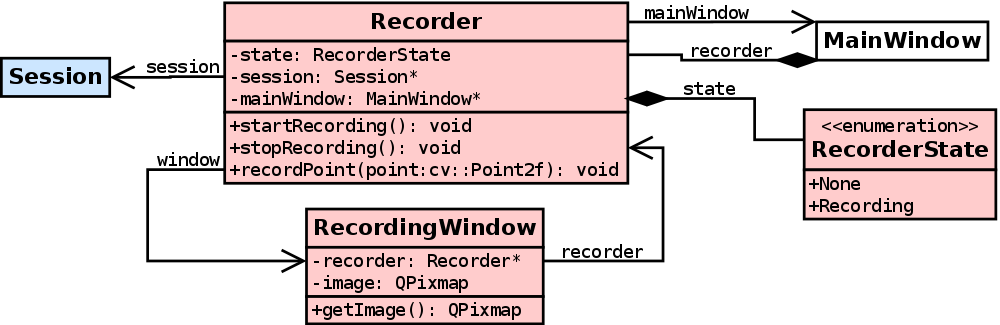
\includegraphics[width=140mm, keepaspectratio]{figures/class_recorder.png}
\end{figure}

A \texttt{Recorder} osztály felelős az új munkamenetek létrehozásáért. Tartozik hozzá egy, a megjelenítést végző ablak, a \texttt{RecordingWindow} osztály egy példánya. Emellett a belső állapot is nyilvántartásra kerül a \texttt{RecorderState} felsorolás értékei által.

Az osztály publikus interfésze mondhatni magától értetődő. A \texttt{startRecording} függvény a meghívását követően azonnal képernyőképet (screenshot) készít az elsődleges kijelző tartalmáról, és elkezdi egy új munkamenet felvételét. A munkamenet azonosítója az alkalmazás jelenlegi állapotában automatikusan a felvétel indításának pillanatában érvényes UNIX időbélyeg (timestamp) értéke lesz.

A \texttt{recordPoint} metódussal új mérési pontot lehet a munkamenethez fűzni. Az alkalmazás használata során a \texttt{recordPoint} függvény felvétel során minden képkocka feldolgozása után meghívódik, vagyis képkockánként egy mérési pont kerül tárolásra. Ennél sűrűbb mintavételnek nyilvánvalóan nincs értelme, de a ritkább pontregisztrálás lehetősége adott.

A \texttt{stopRecording} függvény a felvétel befejeztével hívódik meg. A futása során eltünteti a felvételi ablakot, valamint le is menti az elkészült munkamenetet a háttértárra.

%............................................................................
\subsection{A \texttt{Player} osztály}\label{sect:player}
%............................................................................

\begin{figure}[!ht]
\centering
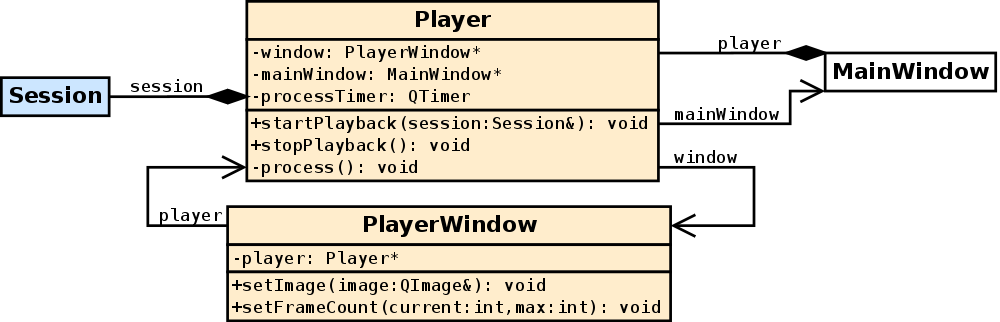
\includegraphics[width=140mm, keepaspectratio]{figures/class_player.png}
\end{figure}

A \texttt{Player} osztály a felvett munkamenetek lejátszásáért felelős. A lejátszást a dinamikusan foglalt \texttt{PlayerWindow} példány grafikus felületén végzi.

A \texttt{startPlayback} metódus egy munkamenet-objektumra (\texttt{Session}) mutató referenciát vár paraméterként, ennek lejátszását kezdi el meghívása után azonnal.

A visszajátszás futása közben a \texttt{processTimer} időzítő és a \texttt{process} függvény gondoskodik a megfelelő ütemben történő visszajátszásról, felhasználva a \texttt{MainWindow} osztály \texttt{PROCESS\_TIMEOUT} értékét. A feldolgozott képet a \texttt{PlayerWindow} osztály \texttt{setImage} metódusának meghívásával jeleníti meg.

A \texttt{stopPlayback} függvény egyszerűen bezárja a használt (teljes képernyős) ablakot, ezzel egy időben leállítja a munkamenet visszajátszását.

%............................................................................
\subsection{A \texttt{Heatmapper} osztály}\label{sect:heatmapper}
%............................................................................

\begin{figure}[!ht]
\centering
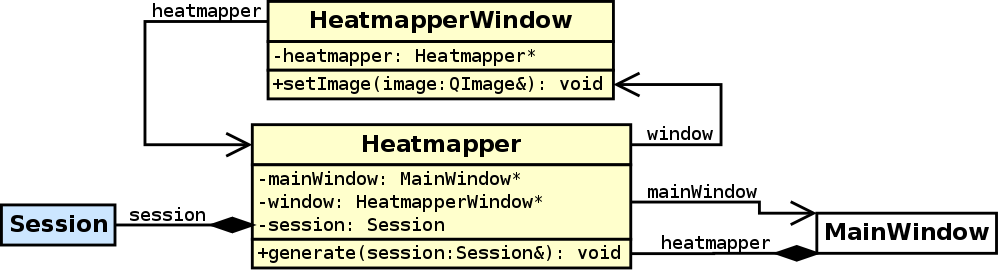
\includegraphics[width=140mm, keepaspectratio]{figures/class_heatmapper.png}
\end{figure}

A \texttt{Heatmapper} osztály a munkamenetekhez kapcsolódó hőtérképek (heatmap) generálására és megjelenítésére szolgál.

Az osztály \texttt{generate} függvénye a paraméterül kapott \texttt{Sesssion} referencia alapján kezdi meg a működését. A generálás meglehetősen hosszú folyamat, ennek végeztével a \texttt{HeatmapperWindow} osztály grafikus felületén jelenik meg a munkamenet hőtérképes reprezentációja.

%............................................................................
\subsection{Kisegítő osztályok}\label{sect:helper}
%............................................................................

Röviden szeretnék szót ejteni az osztálydiagram eddig mellőzött elemeiről is. Ezek az osztályok nem közvetlenül a specifikáció valamely pontjára nyújtanak megoldást, inkább ismétlődő feladatok megoldására adnak helyet.

\paragraph{A \texttt{SessionItemWidget} osztály}

Az osztály a megjelenítésben jut szerephez. A munkamenetek egy listában kerülnek megjelenítésre a főablak bal oldalán. A lista elemeinek egyedi megjelenítésük van, ennek a grafikus elemnek (widget) a felületét tartalmazza a \texttt{SessionItemWidget} osztály.

\paragraph{A \texttt{Helper} osztály}

A kódolás során több helyen is szükség volt különböző átalakítások elvégzésére. A \texttt{Helper} osztály statikus metódusai időbélyegek formázására, valamint a Qt és az OpenCV belső kép-reprezentációi közötti oda-vissza átalakításra szolgálnak.

%,,,,,,,,,,,,,,,,,,,,,,,,,,,,,,,,,,,,,,,,,,,,,,,,,,,,,,,,,,,,,,,,,,,,,,,,,,,,
\section{Grafikus felhasználói felület}\label{sect:gui}
%,,,,,,,,,,,,,,,,,,,,,,,,,,,,,,,,,,,,,,,,,,,,,,,,,,,,,,,,,,,,,,,,,,,,,,,,,,,,

\texttt{+++ leiras + kepek a felhasznalo feluletrol +++}

%,,,,,,,,,,,,,,,,,,,,,,,,,,,,,,,,,,,,,,,,,,,,,,,,,,,,,,,,,,,,,,,,,,,,,,,,,,,,
\section{Felhasználói dokumentáció}\label{sect:docs}
%,,,,,,,,,,,,,,,,,,,,,,,,,,,,,,,,,,,,,,,,,,,,,,,,,,,,,,,,,,,,,,,,,,,,,,,,,,,,

Az alkalmazás indítása után a felhasználót a főablak fogadja. Az ablak bal oldalán a felvett munkamenetek megtekintésére, törlésére, lejátszására, illetve hőtérkép generálására van lehetőség. A főablak jobb oldalán van lehetőség új munkamenetek rögzítésére.

\paragraph{Munkamenet felvétele}

\begin{enumerate}
  \item Adjuk fel a vizsgálandó alanyra a sapkát, amelyhez a webkamera rögzítve van!
  \item Végezzük el a kamerakép bekapcsolását a \textbf{Start} gomb megnyomásával (gyorsbillenyű: \textbf{S})!
  \item Győződjünk meg róla, hogy a kamera orientációja megfelelő: ha nem, irányítsuk a szemrégióra!
  \item Szükség esetén állítsuk be a kamera fókuszát a lencse tekerésével úgy, hogy a pupilla a lehető legélesebben rajzolódjon ki!
  \item Kérjük meg az alanyt, hogy a vizsgálat során csak a szemét mozgassa, a fejét ne! A pontosabb mérés érdekében használhatunk álltámaszt is.
  \item Indítsuk a kalibrációt a \textbf{Calibrate} gomb megnyomásával (gyorsbillentyű: \textbf{C})!
  \item A kalibráció során kérjük meg az alanyt, hogy tekintetét irányítsa a képernyő sarkain sorban megjelenő céltáblákra! A kalibrációs pont rögzítését a céltáblára kattintva, vagy az \textbf{Enter} gyorsbillentyű segítségével végezhetjük.
  \item A háttérben jelenítsük meg a vizsgálni kívánt képet (pl. weboldal részlete).
  \item A \textbf{Record} gomb megnyomásával indítsuk el a munkamenet felvételét (gyorsbillentyű: \textbf{R})
  \item A felvételt a \textbf{Record} gomb újbóli megnyomásával, vagy az \texttt{Escape} gyorsbillentyűvel állíthatjuk le.
\end{enumerate}

\paragraph{Munkamenet visszajátszása}

\begin{enumerate}
  \item Válasszuk ki a bal oldali listából a visszajátszani kívánt munkamenetet!
  \item Kattintsunk a \texttt{Play} gombra! A visszajátszás megkezdődik, és folyamatosan ismétlődik, amíg le nem állítjuk.
  \item A visszajátszás leállításához nyomjuk meg az \textbf{Escape} billentyűt!
\end{enumerate}

\paragraph{Hőtérkép generálása}

\begin{enumerate}
  \item Válasszuk ki a bal oldali listából azt a munkamenetet, amelyhez hőtérképet szeretnénk generálni!
  \item Kattintsunk a \textbf{Heatmap} gombra! A generálás megkezdődik, a folyamat állása a státuszsávon visszajelzésre kerül. A generálás végeztével a hőtérkép megjelenik a képernyőn.
  \item Használjuk az \textbf{Escape} billentyűt a hőtérkép bezárásához.
\end{enumerate}

\paragraph{Többmonitoros használat}

A program fel lett készítve a több monitorral történő használatra. Amennyiben nem a saját tekintetünket követjük, hanem egy másik felhasználóét (alany), úgy a kétmonitoros elrendezés használata a legkényelmesebb.

Az alkalmazás főablakát húzzuk a másodlagos monitorra, ez lesz a vizsgáló képernyője. Az elsődleges monitort használjuk az alany képernyőjeként, azon jelenítsük meg a vizsgálni kívánt ábrákat, képeket, weboldal-részleteket stb. A másodlagos monitoron a vizsgáló a mérés teljes időtartama alatt szemmel tarthatja az alkalmazás főablakát. Ennek köszönhetően például azt is figyelemmel kísérheti, hogy a kamera vagy a fej elmozdulásából kifolyólag a kalibráció a mérés során (vagy két mérés között) helytelenné válik-e. Amennyiben igen, kérheti új kalibráció elvégzését és a mérés megismétlését.

%,,,,,,,,,,,,,,,,,,,,,,,,,,,,,,,,,,,,,,,,,,,,,,,,,,,,,,,,,,,,,,,,,,,,,,,,,,,,
\section{Tesztelés, eredmények}\label{sect:teszteles}
%,,,,,,,,,,,,,,,,,,,,,,,,,,,,,,,,,,,,,,,,,,,,,,,,,,,,,,,,,,,,,,,,,,,,,,,,,,,,

\texttt{+++ tesztelesi dokumentacio (ide mit?) +++}
\include{chapter7}
%----------------------------------------------------------------------------
\chapter*{Értékelés}\label{sect:ertekeles}
%----------------------------------------------------------------------------

A diplomatervem elkészítése kétségkívül összetett és kihívásokkal teli feladat volt. A szakirodalom feldolgozásával és a megszerzett ismeretek összefoglalásával jó rálátásom nyílt a kutatási terület legfontosabb részeire, ennek köszönhetően magabiztosan tudtam belevágni a pupillakövetésre használható módszerek megismerésébe. Az egyes módszerek implementálásával és összehasonlításával -- útközben sok hasznos tanulságot leszűrve --, úgy gondolom, sikerült a feladat megoldásának legjobb módját kiválasztanom.

A tervezés és megvalósítás során a rendelkezésemre álló hardver- és szoftvereszközök ötvözésével olyan rendszert sikerült implementálnom, amely már kezdeti formájában is eléri célját: megfelelő sebességgel és minőségben képes a tekintet követésére.

\bigskip

Az elkészített rendszer természetesen számos irányban továbbfejleszthető. A fejlesztések egyrészt irányulhatnak a hardvereszközök módosítására illetve cseréjére, valamint a szoftveres feldolgozás és leképezés javítására.

Hardverszempontból az egyik fejlesztést igénylő pont magától értetődően a látóteret viszonylag nagy mértékben kitakaró webkamera problémájának megoldása lehet. A kamera szempontunkból ,,hasznos'' részei csak maga a lencse, az érzékelő, valamint a megvilágítást szolgáltató LED-ek. Ezek helyigénye más kamera beszerzésével, illetve akár egyedi hardver tervezésével minimalizálható lehet.

A felhasználó számára jelenleg kényelmetlenséget jelent, hogy a tekintetkövetés során a fej nem mozgatható, a legpontosabb követés érdekében pedig ajánlott az álltámasz használata. A fejmozgás hat szabadságfokú követésével -- például ultrahangos vagy sztereó módszerek használatával -- a fejmozgás szabadsága biztosítható lehet. 

A rendszer mostani megvalósításában a kamera képfrissítési sebessége szintén egy szűk keresztmetszet. A 30 képkockás másodpercenkénti sebességnél gyorsabb kamera használatával jóval finomabb szemmozgások is megfigyelhetőek lennének.

\bigskip

A feldolgozást végző szoftver fejlesztése is több irányban folytatható. A felhasználói aktivitás könnyebben mérhetővé válna, ha mindössze egy darab rögzített kép helyett a munkamenetek alatt a képernyő tartalmának változása is tárolásra kerülne. Ennek megvalósításában komoly feladatnak bizonyulhat a videofolyam élő rögzítése és tömörítése (a helyfoglalás optimalizálásának érdekében) úgy, hogy az a tekintetkövetés sebességét ne befolyásolja.

A szoftveres feldolgozás sebességének javítására igazából csak gyorsabb képfrissítésű kamera használata esetén lenne szükség. Ha felmerül az igény a nagyobb sebességű feldolgozásra, akkor a használt algoritmusok párhuzamosítása egy olyan irány, amelyben érdemes lehet a rendszert továbbfejleszteni. Modern hardverekkel (pl. GPU-gyorsítás használatával) az előfeldolgozási és követési lépések végrehajtása akár többszörös sebességre gyorsítható.

A jelenlegi implementáció pontossági hibáját orvosolandó szükség lenne a kalibráció és a leképezési algoritmus finomítására. A javítás egy lehetséges módja, hogy a négypontos kalibráció helyett akár kilenc, tizenhat, huszonöt stb. kalibrációs pontot felhasználva próbáljuk meg kiküszöbölni a bilineáris interpoláció pontatlanságát. Esetleg szóba jöhet a felhasznált lineáris interpolációra alapuló módszer elvetése, és ahelyett a szemgolyó formáját és forgását pontosabban modellező leképezési módszer bevezetése.
%----------------------------------------------------------------------------
\chapter*{Köszönetnyilvánítás}
%----------------------------------------------------------------------------

Ezúton szeretném megragadni az alkalmat, hogy köszönetet mondjak mindazoknak, akik a diplomatervem elkészítéséhez hozzájárultak.

\bigskip

Mindenekelőtt köszönetemet fejezném ki konzulensem, Kertész Zsolt kitartó támogatásáért, valamint elméleti és gyakorlati szinten is rendkívül hasznos meglátásaiért.

Továbbá szeretném megköszönni családom tagjainak türelmét és támogatását, különös tekintettel a rendszer tesztelése során tanúsított aktív és szíves részvételükre.

%\phantomsection\markboth{Ábrák jegyzéke}{}\listoffigures\newpage
%\phantomsection\markboth{Táblázatok jegyzéke}{}\listoftables\newpage

\phantomsection\markboth{Irodalomjegyzék}{}\bibliography{mybib}
%\addcontentsline{toc}{chapter}{Irodalomjegyzék}
\bibliographystyle{unsrt}

%----------------------------------------------------------------------------
\appendix
%----------------------------------------------------------------------------
\chapter*{Függelék}
\setcounter{chapter}{6}  % a fofejezet-szamlalo az angol ABC 6. betuje (F) lesz
\setcounter{equation}{0} % a fofejezet-szamlalo az angol ABC 6. betuje (F) lesz
\numberwithin{equation}{section}
\numberwithin{figure}{section}
\numberwithin{lstlisting}{section}
\numberwithin{table}{section}
\setcounter{footnote}{0}

%,,,,,,,,,,,,,,,,,,,,,,,,,,,,,,,,,,,,,,,,,,,,,,,,,,,,,,,,,,,,,,,,,,,,,,,,,,,,
\section{Mellékletek}\label{sect:mellekletek}
%,,,,,,,,,,,,,,,,,,,,,,,,,,,,,,,,,,,,,,,,,,,,,,,,,,,,,,,,,,,,,,,,,,,,,,,,,,,,

%Jelen dokumentum, a féléves munkát bemutató prezentáció, valamint az alkalmazás forráskódja, elérhetők az Interneten is, a \url{http://mozes.info/pupilmeasure/} címen.

%Az alkalmazás forráskódja a \url{https://github.com/obrien/pupilmeasure} címen található GitHub\footnote{\url{http://github.com/}} projektben is elérhető és felhasználható.

%,,,,,,,,,,,,,,,,,,,,,,,,,,,,,,,,,,,,,,,,,,,,,,,,,,,,,,,,,,,,,,,,,,,,,,,,,,,,
\section{Telepítés}\label{sect:telepites}
%,,,,,,,,,,,,,,,,,,,,,,,,,,,,,,,,,,,,,,,,,,,,,,,,,,,,,,,,,,,,,,,,,,,,,,,,,,,,

%Az alkalmazás fordítása az alábbi verziójú programokkal történt:

%\begin{itemize}
%\item g++ --  4.4.5
%\item OpenCV -- 2.1.0
%\item wxWidgets -- 2.8.10
%\end{itemize}

%A  2.1.0 verziójú \textit{OpenCV} könyvtár forráskódja az \url{http://opencv.willowgarage.com/wiki/} címről letölthető. Az ennél újabb verziók interfészébe nem került bele a működéshez elengedhetetlenül szükséges \texttt{cvSnakeImage} függvény, ezért az alkalmazás mindenképpen a fenti verziójú \textit{OpenCV} könyvtár meglétét igényli! A fordításhoz szükséges csomagok a használt disztribúció csomagkezelőjéből elérhetők az \listref{install} listában felsorolt (vagy ahhoz hasonló) néven.

%\begin{lstlisting}[frame=single,float=!ht,caption=Az OpenCV fordításához szükséges csomagok telepítése,label=listing:install]
%sudo apt-get install libgtk2.0-dev libunicap2-dev libucil2-dev libswscale-dev \\
%libdc1394-22-dev libv4l-dev libxine-dev libavformat-dev libglut3-dev \\
%libwxgtk2.8-dev
%\end{lstlisting}

%A \emph{Pupil Measure} alkalmazás fordítása ezek után a forráskód könyvtárában kiadott \texttt{make} paranccsal történhet. A lefordított bináris a \texttt{./pupilmeasure} parancs kiadásával indítható, de előtte az \texttt{LD\_LIBRARY\_PATH} környezeti változóba a \texttt{usr/local/lib} érték betöltendő!


\label{page:last}
\end{document}
